% TO-DO:
% * What does --> in a topos correspond to in FOL or HOL?

\documentclass[12pt, orivec]{article}
\usepackage{amsmath}
\usepackage{amssymb}    % for \rightsquigarrow
\usepackage{wasysym}	% for frown face
\usepackage{mathrsfs} 	% for \mathscr
\usepackage{stmaryrd}
\usepackage[most]{tcolorbox}
\usepackage{ulem}
\usepackage{tikz-cd}		% commutative diagrams
\usepackage{tikz}
\usepackage{amsthm}
\usepackage{enumitem}	% for \itemize custom labels
\usepackage{turnstile}	% longer turnstiles
\usepackage[sf,bf,big,raggedright,compact]{titlesec}	% change section color to blue
\usepackage[backend=biber,bibstyle=authoryear,citestyle=authoryearbrack]{biblatex}
\bibliography{../AGI-book}

\newtheorem{theorem}{Theorem}

\ifdefined\chinchin
\usepackage[CJKspace]{xeCJK}
\setCJKmainfont[BoldFont=SimHei,ItalicFont=AR PL KaitiM GB]{SimSun}
\newcommand{\cc}[2]{#1}
\else
\newcommand{\cc}[2]{#2}
\fi

\setlength{\headheight}{0cm}
\setlength{\hoffset}{0cm}
\setlength{\topmargin}{-2cm}
\setlength{\oddsidemargin}{-2cm}
\setlength{\evensidemargin}{-2cm}
\setlength{\textwidth}{20cm}
\setlength{\textheight}{26cm}
\setlength{\headsep}{0cm}
\setlength{\topskip}{0cm}
\setlength{\footskip}{0.9cm}  % between bottom of page and page number
\setlength{\floatsep}{0cm}
\setlength{\textfloatsep}{0.6cm}
\setlength{\intextsep}{0.5cm}
\setlength{\parindent}{0em}   % em = width of capital M


% Fix spilling of titles in bibliography:
\DeclareFieldFormat*{title}{#1}

\DeclareFieldFormat*{titlecase}{%
    \ifdef{\currentfield}
      {\ifcurrentfield{title}
         {\usefield{\uline}{\currentfield}}%
         {#1}}
      {#1}}

\setcounter{secnumdepth}{0}		% no section numbers

\titleformat{\section}[hang]{\bfseries\Large\color{blue}}{\thesection \hspace{10pt}}{0pt}{}
\titleformat{\subsection}[hang]{\bfseries\large\color{blue}}{\thesubsection \hspace{5pt}}{0pt}{}

\newcommand{\book}[1]{$\NewSym[0.4]{../book-icon.png} \quad$ \parbox{0.9\textwidth}{\footnotesize #1}}
\newcommand{\code}[1]{{\footnotesize{\ttfamily #1}}}
\newcommand{\tab}{\hspace*{2cm}}
\newcommand{\powerset}{\raisebox{.15\baselineskip}{\Large\ensuremath{\wp}}}
\newcommand{\Chi}{\raisebox{2.5pt}{$\chi$}}
\newcommand*\KB{\vcenter{\hbox{\includegraphics{../KB-symbol.png}}}}
\newcommand*\NewSym[2][0.5]{\vcenter{\hbox{\includegraphics[scale=#1]{#2}}}}
\newcommand*\sigmoid{\vcenter{\hbox{
\includegraphics{../sigmoid.png}}}}
\newcommand{\smbox}[1]{\boxed{\footnotesize{\mbox{#1}}}}

\newcommand{\tikzmark}[1]{\tikz[overlay,remember picture] \node (#1) {};}

\newcommand{\Dfrac}[2]{%
\ooalign{%
      $\genfrac{}{}{2.9pt}0{\hphantom{#1}}{\hphantom{#2}}$\cr%
      $\color{white}\genfrac{}{}{1.5pt}0{\hphantom{#1}}{\hphantom{#2}}$\cr%
      $\color{white}\genfrac{}{}{1pt}0{\color{black}#1}{\color{black}#2}$}}

\renewcommand{\thefootnote}{\fnsymbol{footnote}}
\interfootnotelinepenalty=10000

\title{\cc{人工智能的知识表述}{Knowledge representation in AI}}
\author{\cc{甄景贤}{Yan King Yin} {\footnotesize general.intelligence@gmail.com}}

\begin{document}
\setlength{\parindent}{0pt}
\setlength{\parskip}{2.8ex plus0.8ex minus0.8ex}

\maketitle

\tableofcontents

\begin{abstract}
At the top level, an AI can be construed as a dynamical system moving in ``cognitive space'', trying to minimize a loss function (or maximize a reward).  The control of such a system follows the Hamilton-Jacobi-Bellman equation.  This framework of reinforcement learning does not offer sufficient structure to solve the AI problem effectively, but it provides a perspective from which subsequent development is possible.

The salient feature of human intelligence is reasoning ability, which is distilled as the theory of logic.  We need to impose this logical structure on the AI system (ie, inductive bias).  Topos theory provides the perfect abstraction tool to do this.  Recently, Google / DeepMind proposed a reasoning architecture based on a neural network acting upon a graph memory.  With our abstraction we may be able to improve upon the graph model with simpler and perhaps more efficient ``geometric models''.  The categorical perspective makes it easier to see the problem's structure.

The abstract formulation of AI may lead to better variations.  In this paper we look at 3 approaches, based on: A) genetic algorithm; B) neural networks; C) geometric models.  This paper is written in a tutorial style as the mathematical background may be unfamiliar to many AI practitioners or researchers.

%\cc{
%目前(2018 年8月)强人工智能的发展,问题已经不再是「能不能做到」,而是到了「哪个方案比较好」的地步。 本文介绍知识表述的理论,并提出几个解决方案,分别基於: A)基因算法; B)神经网络-知识图混合; C) 几何模型。
%}{
%As of now (2018 August), the question of strong AI is no longer whether it is possible or not, but whether one feasible approach is better than another.  The tutorial introduces the mathematical theory of knowledge representations, and discusses 3 proposals, respectively based on:  A) genetic algorithms;  B) neural networks + graphs;  C) geometric models.
%}
\end{abstract}

\section{\cc{什么是 model theory?}{What is model theory?}}

\cc{
举例来说,hyperbolic geometry(双曲几何)可以「实现」为某些 \textbf{模型}:
}{
For example, \textbf{hyperbolic geometry} can be ``realized'' by the following \textbf{models}:
}
\begin{equation}
\vcenter{\hbox{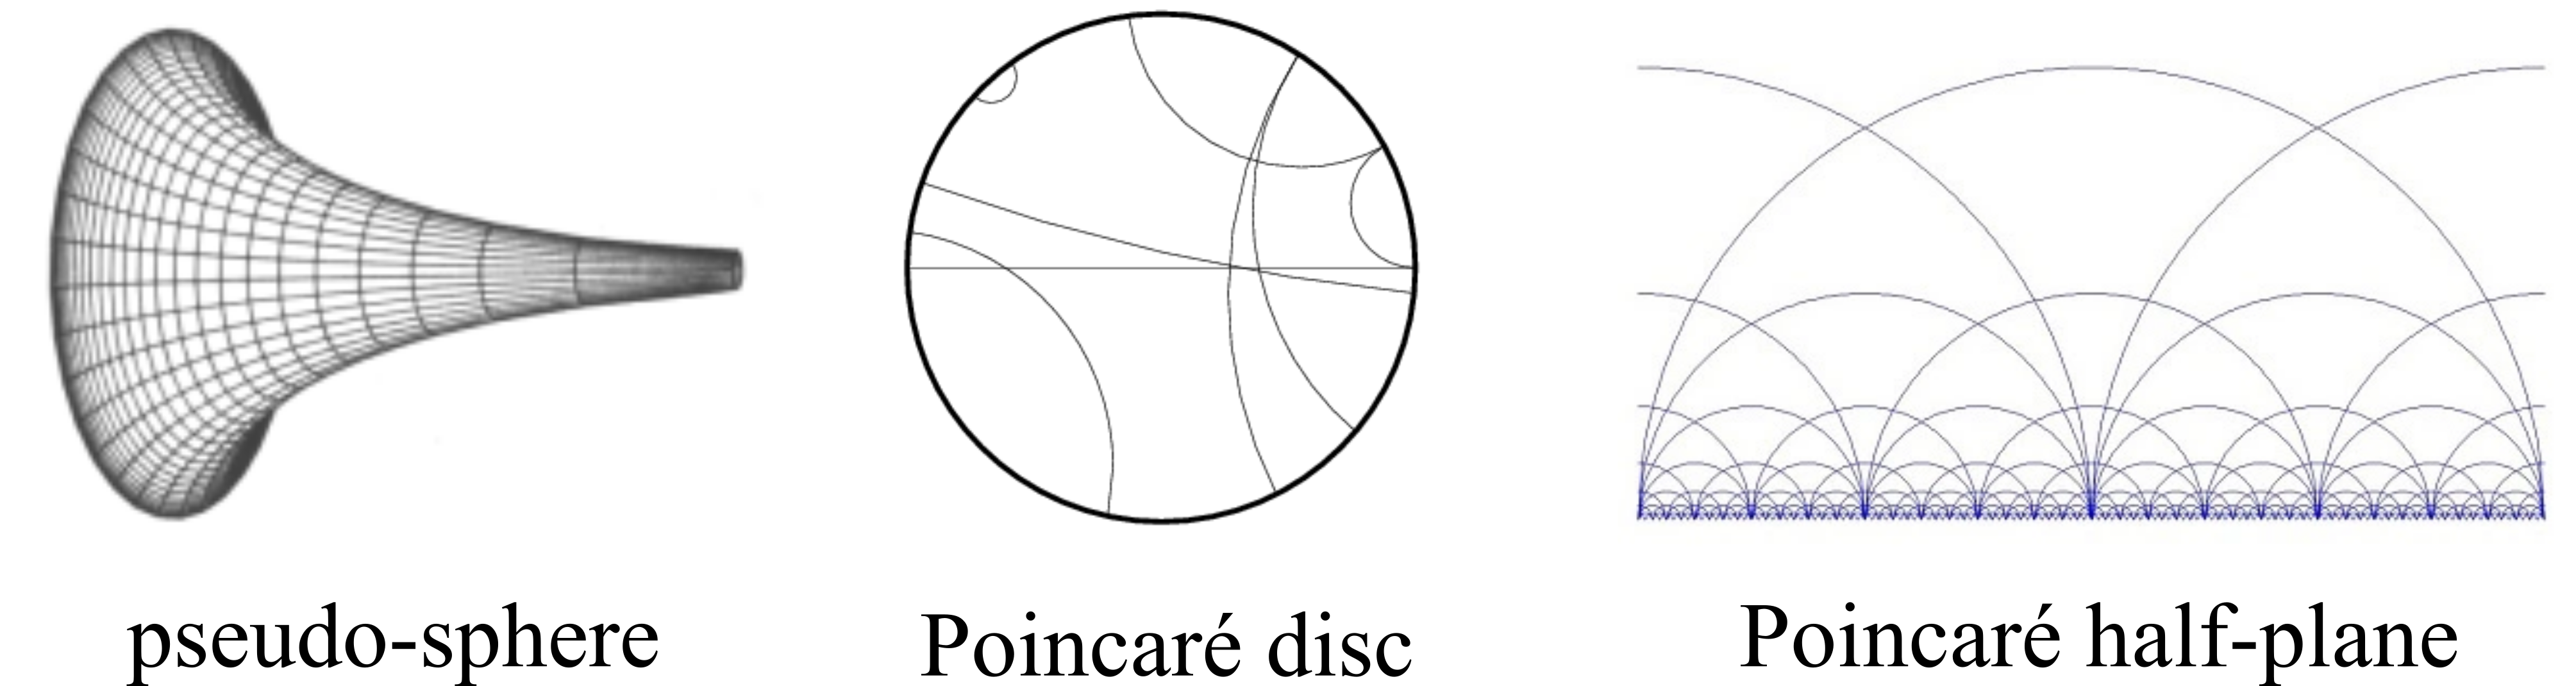
\includegraphics[scale=0.65]{hyperbolic-models.png}}} 
\end{equation}
\cc{
模型不是唯一的,可以有很多种。
}{
Models are not unique, there can be many models for a theory.
}

\cc{
在数理逻辑中,\textbf{模型论} 研究的是 \textbf{syntax} 和 \textbf{model} 之间的 \textbf{对偶}。
}{
In mathematical logic, \textbf{model theory} studies the \textbf{duality} between \textbf{syntax} and \textbf{models}.
}

\cc{
最经典的例子是 \textbf{Stone duality},也是大家熟悉的 ``Venn diagram'':
}{
The most classic example is \textbf{Stone duality}, also familiar to all of us as ``Venn diagrams'':
}
\begin{equation}
P \wedge Q \quad \cong \quad
\vcenter{\hbox{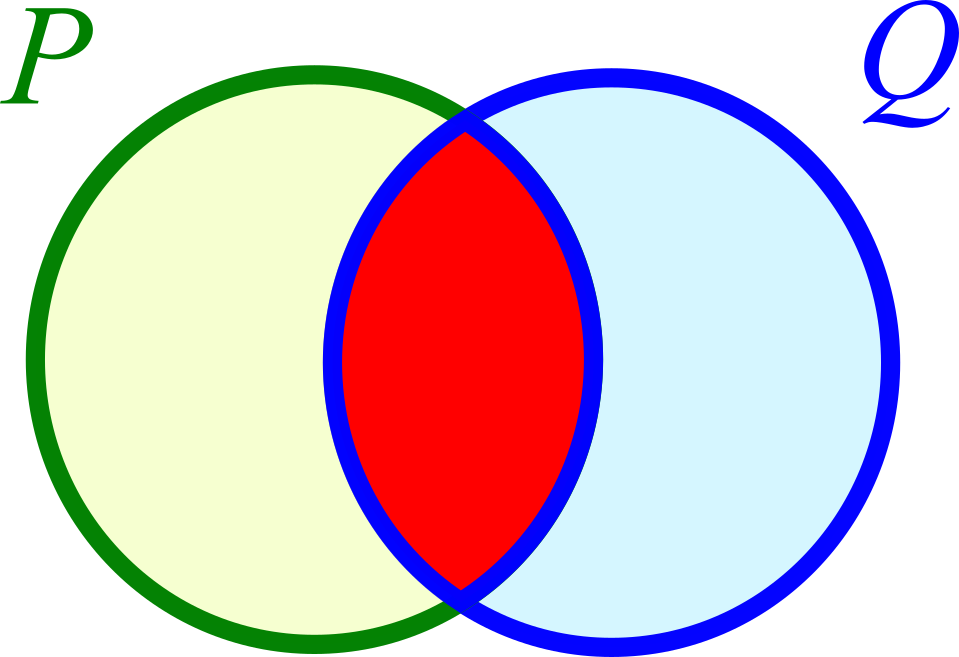
\includegraphics[scale=0.7]{Venn-diagram-0.png}}}
\end{equation}
Stone duality\footnote{Marshall Stone (1903-1989), American mathematician who contributed to real analysis, functional analysis, topology and the study of Boolean algebras.} 
\cc{
指的是 Boolean algebra 和 topological space 之间的对偶。  
}{
refers to the duality between \textbf{Boolean algebras} and \textbf{topological spaces}.
}

\cc{
Boolean algebra 即\textbf{命题逻辑},它只关心命题的 真假,例如 P =「北京正在下雨」,但它不能 ``access'' 命题内部的结构,例如「北京」和「雨水」等成分。 强人工智能最关键的障碍 (obstruction),是命题逻辑到一阶逻辑的跃升 (lifting)。 
}{
Boolean algebra is the same as \textbf{propositional logic}, which concerns only with the truth and falsehood of propositions.  For example, P = \textit{``It is raining in New York''}, but we cannot ``access'' the internal constituents of the propositioon, such as \textit{``rain''} and \textit{``New York''}.  The critical obstruction to strong AI is the \textbf{lifting} from propositional to first-order logic.
}

Roughly speaking, classical logic consists of 2 key notions:
\begin{itemize}
\item \textbf{propositions} are things that can be assigned \textbf{truth values}
\item each proposition is a \textbf{relation} between \textbf{objects}
\end{itemize}
By an informal argument, any idea that is \textit{expressible} in natural language, must be structurally essentially equivalent to predicate logic, which we know from the study of linguistics.  So there is no \textit{concievable} way for us to invent an alternative logic that is drastically different from classical logic, with the exception of relatively simple syntactic transformations.

Alan Turing (1912-1954), being very ahead of his time, \textbf{circumcribed} the problem of AI by formulating the form of all computable functions, ie, Turing machines, later shown to be equivalent to $\lambda$-calculus and combinatory logic.  Figure (\ref{world-of-logical-structures}) shows the family of major logical structures.

\begin{figure*}[htp]	% htp = here, top, page-of-float, for some reason it means `next page`
\begin{equation}
\label{world-of-logical-structures}
% \vcenter{\hbox{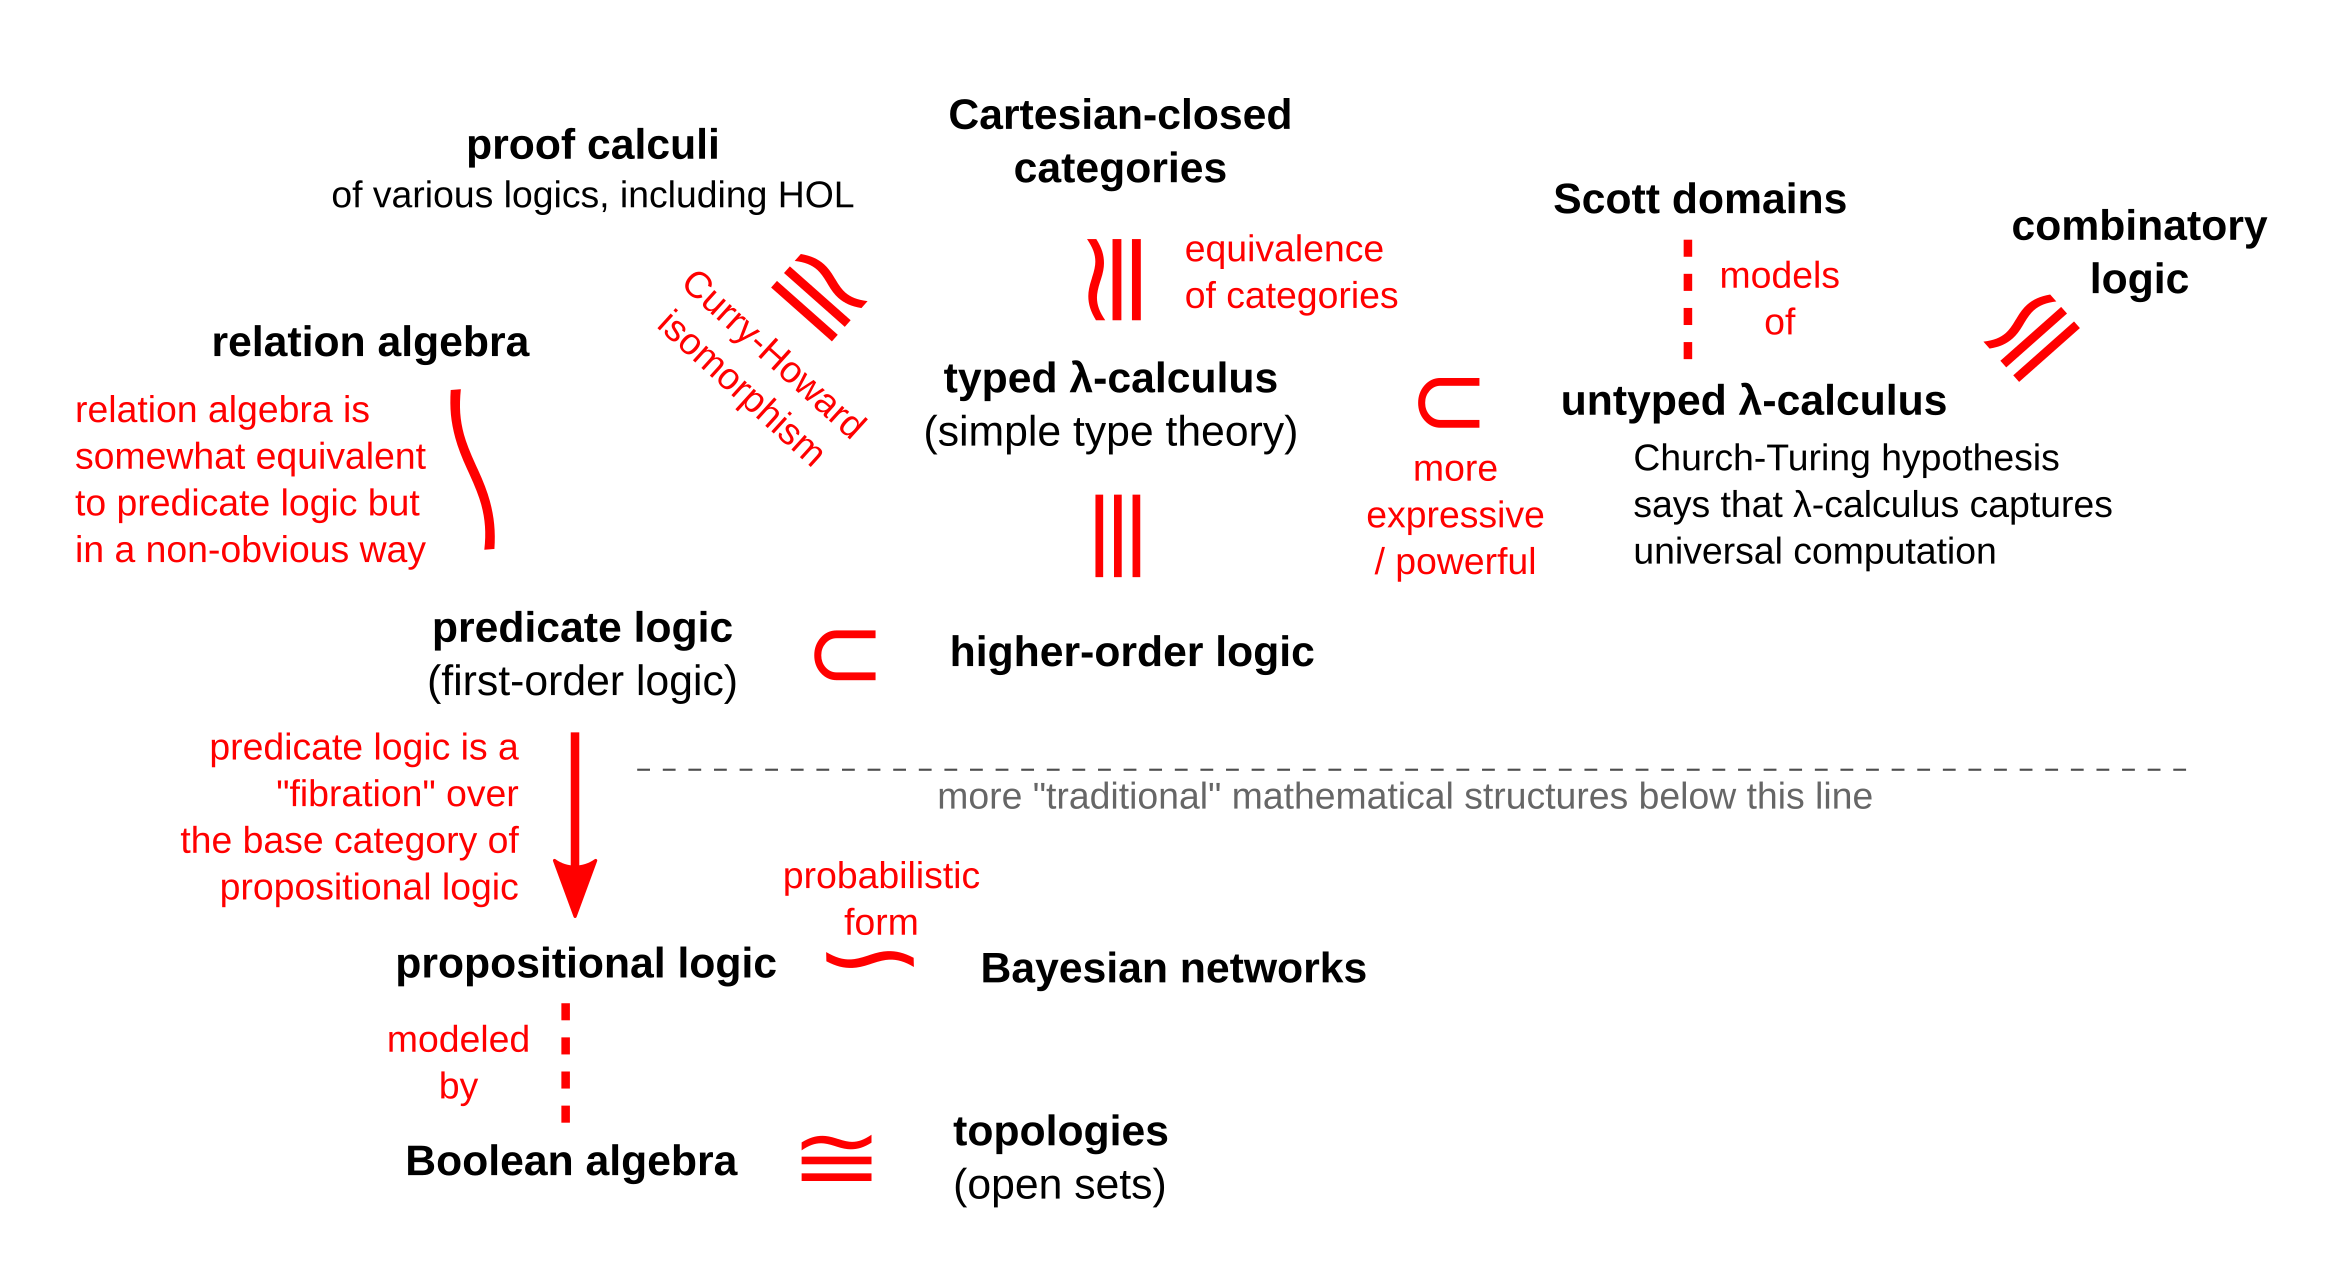
\includegraphics[scale=0.6, angle=-90]{world-of-logical-structures.png}}}
\vcenter{\hbox{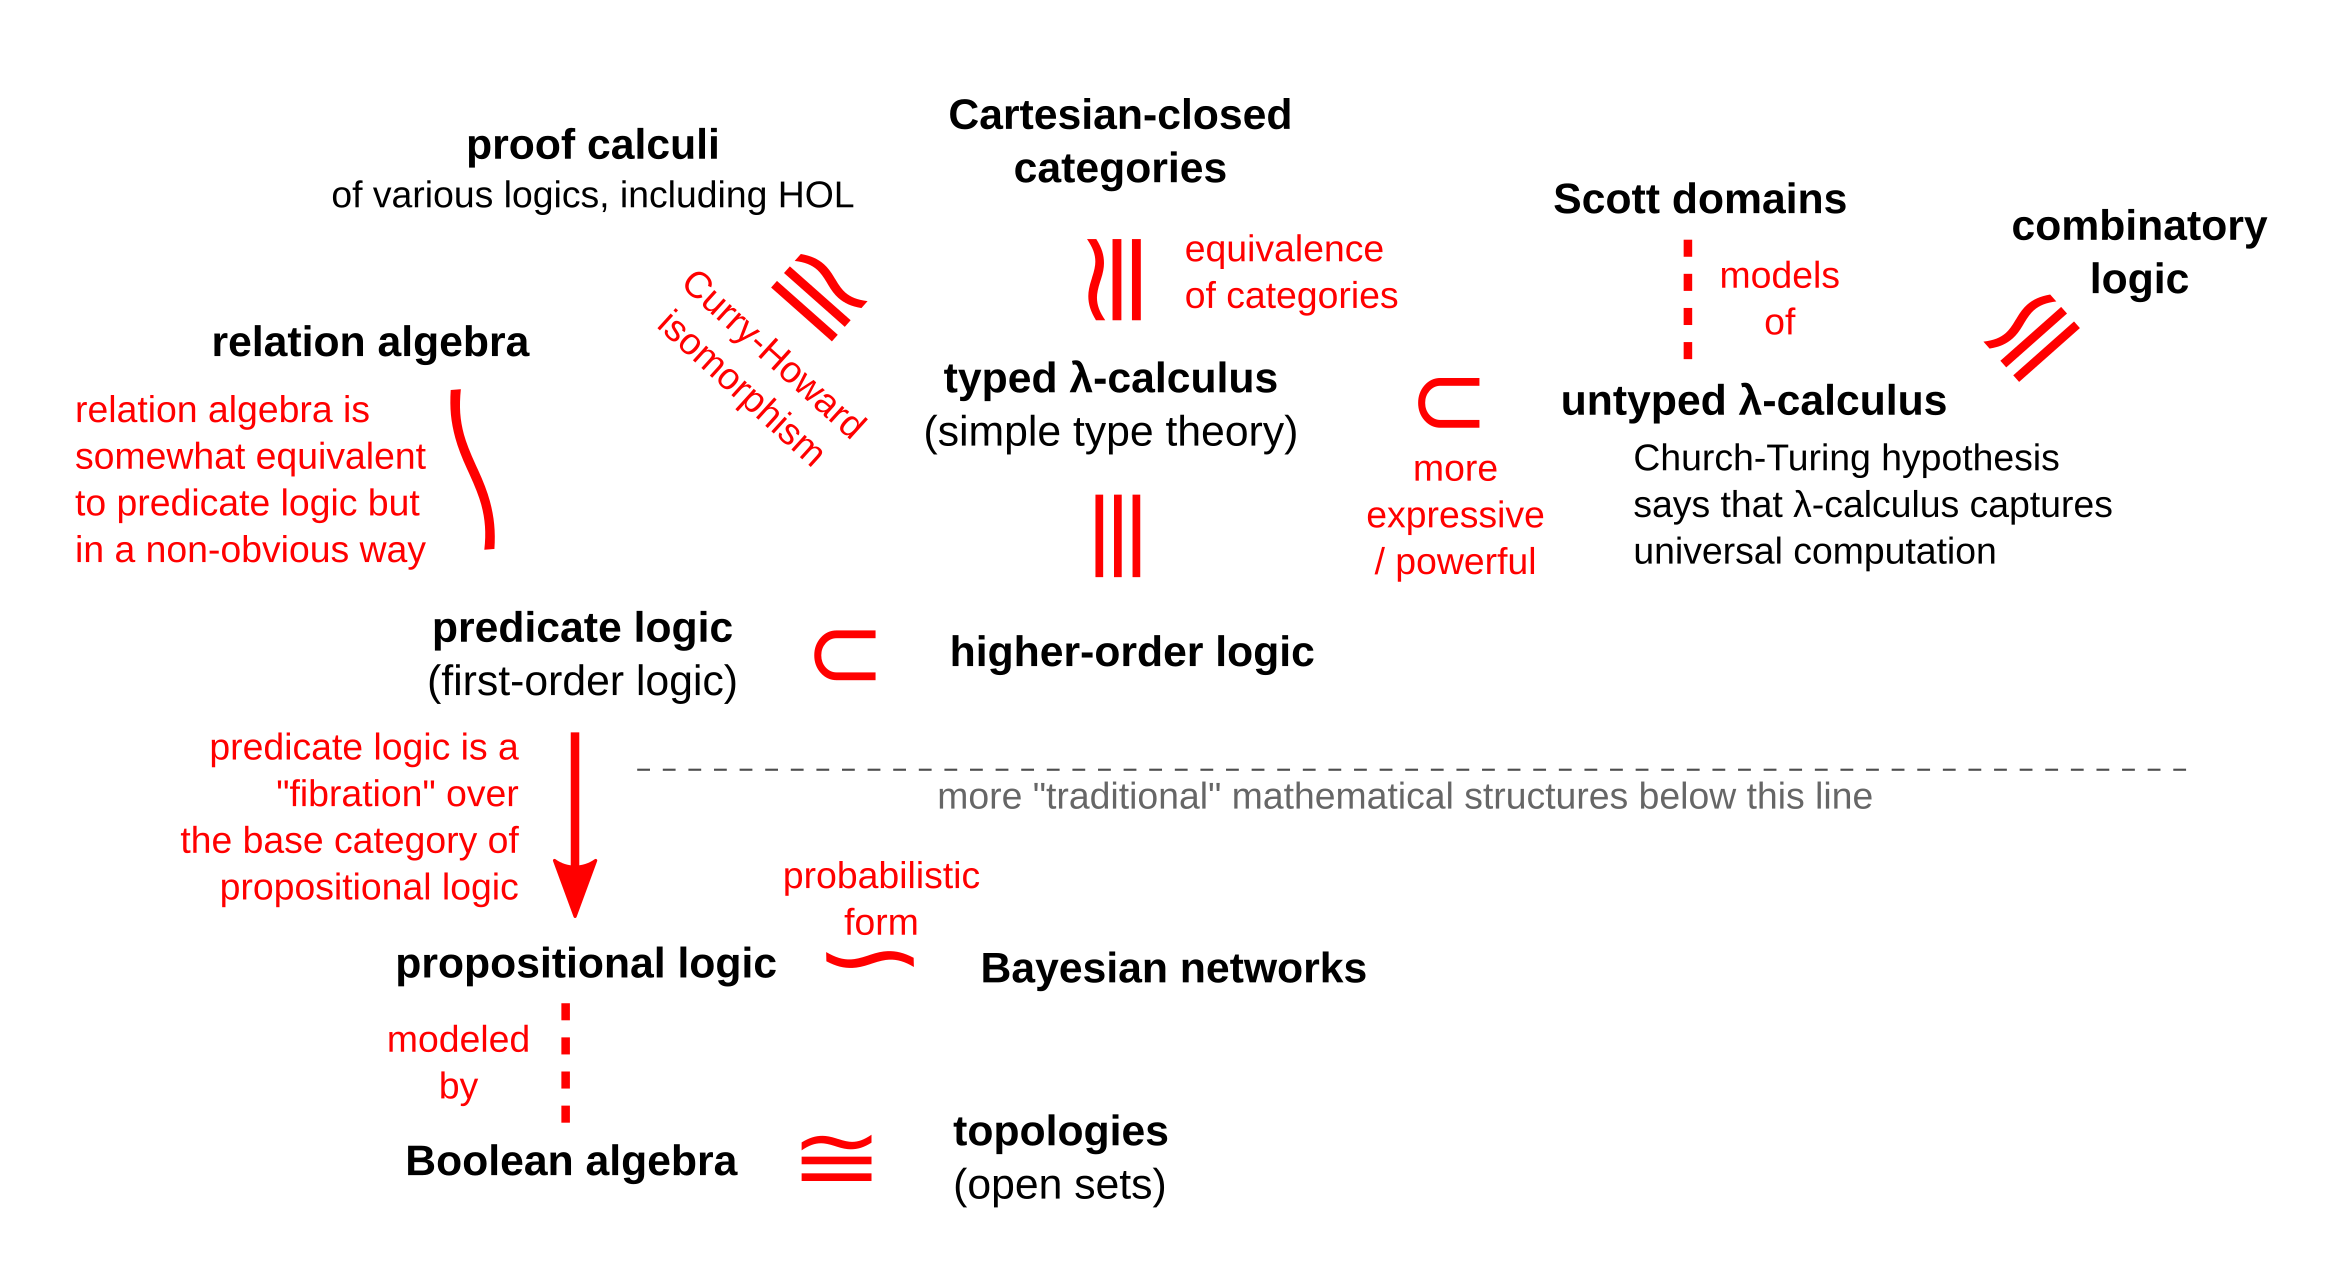
\includegraphics[scale=0.6]{world-of-logical-structures.png}}}
\end{equation}
\end{figure*}

\cc{
First-order logic 的 模型 可以用一些 \textbf{集合} 及其 \textbf{元素} 组成。  例如,\\
}{
First-order logic can be modeled by \textbf{sets} and their \textbf{elements}.  For example \\
}
$\mbox{John} \in \mbox{Male}, \quad \mbox{John, Mary} \in \mbox{Mathematician}$: 
\begin{equation}
\vcenter{\hbox{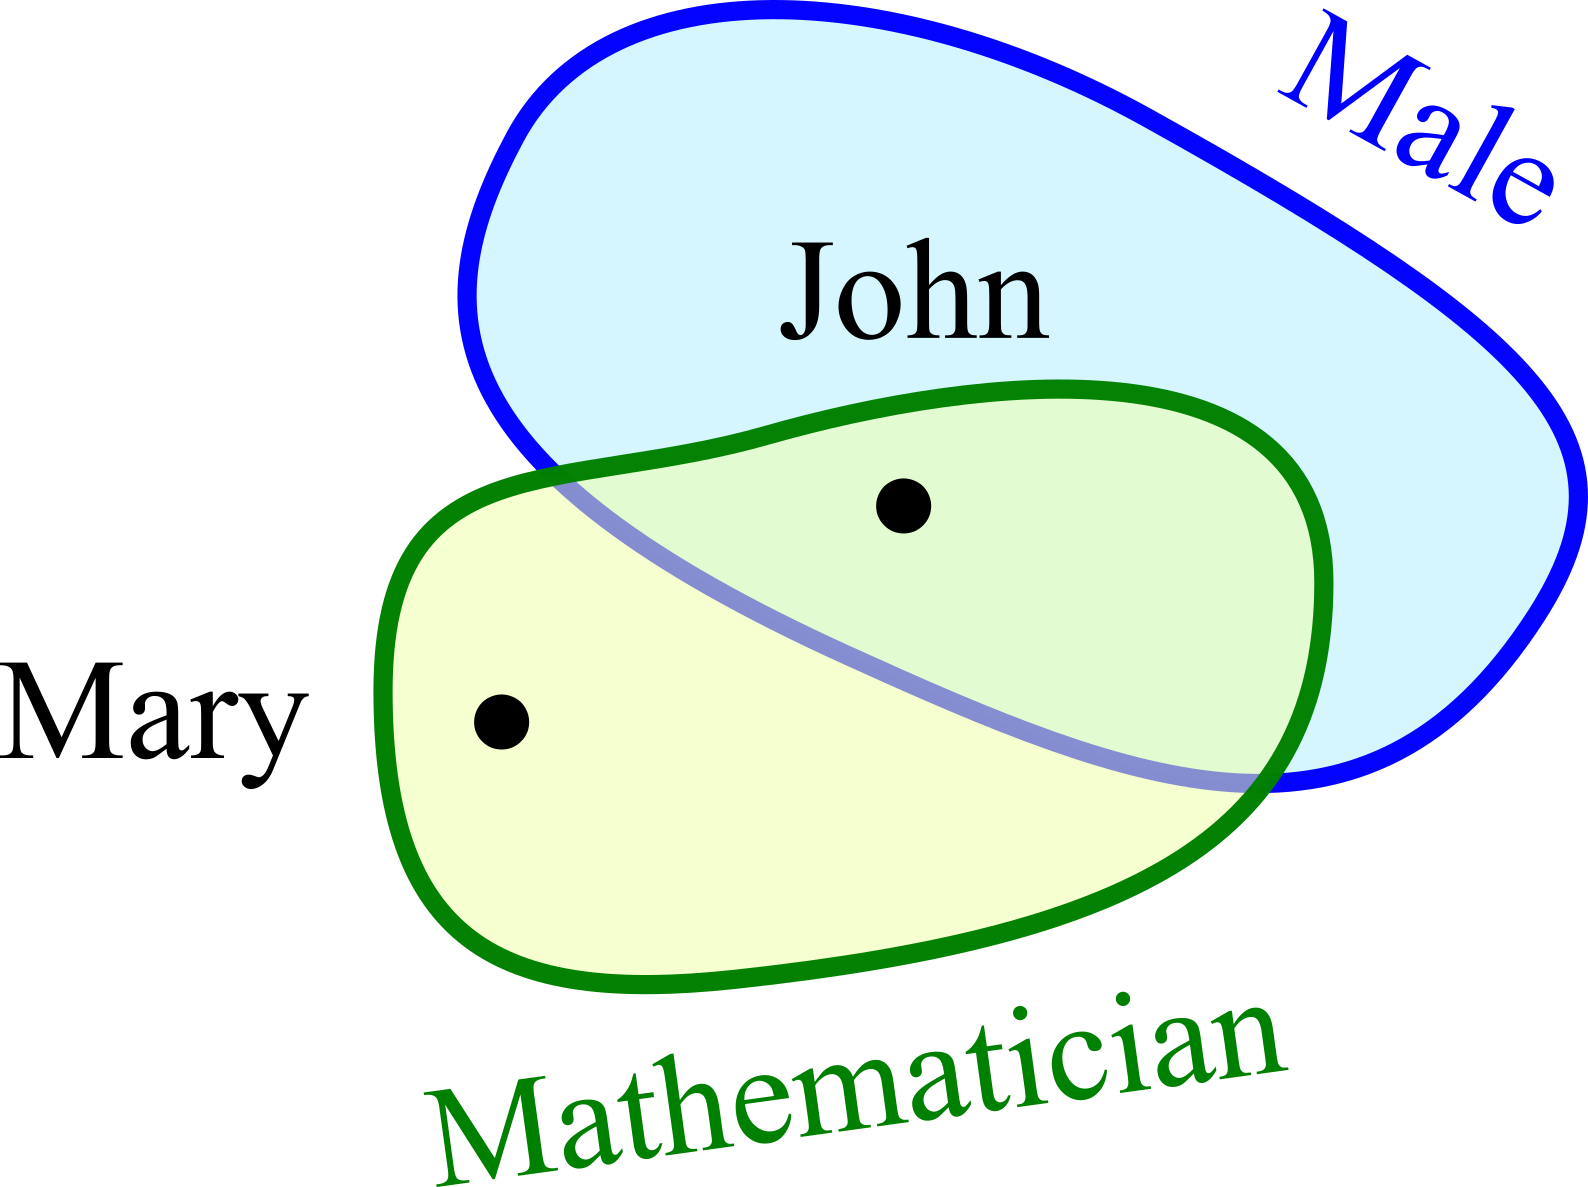
\includegraphics[scale=0.6]{FOL-model-1.png}}} 
\end{equation}
\cc{
而 first-order objects(\textbf{个体})之间的 \textbf{关系} 是 domain $D$ 的 Cartesian product $D \times D$ 内的一些 \textbf{子集},例如:
}{
Whereas \textbf{relations} between first-order \textbf{objects} in a domain $D$ are represented by \textbf{subsets} of the Cartesian product $D \times D$, eg:
}
\begin{equation}
\vcenter{\hbox{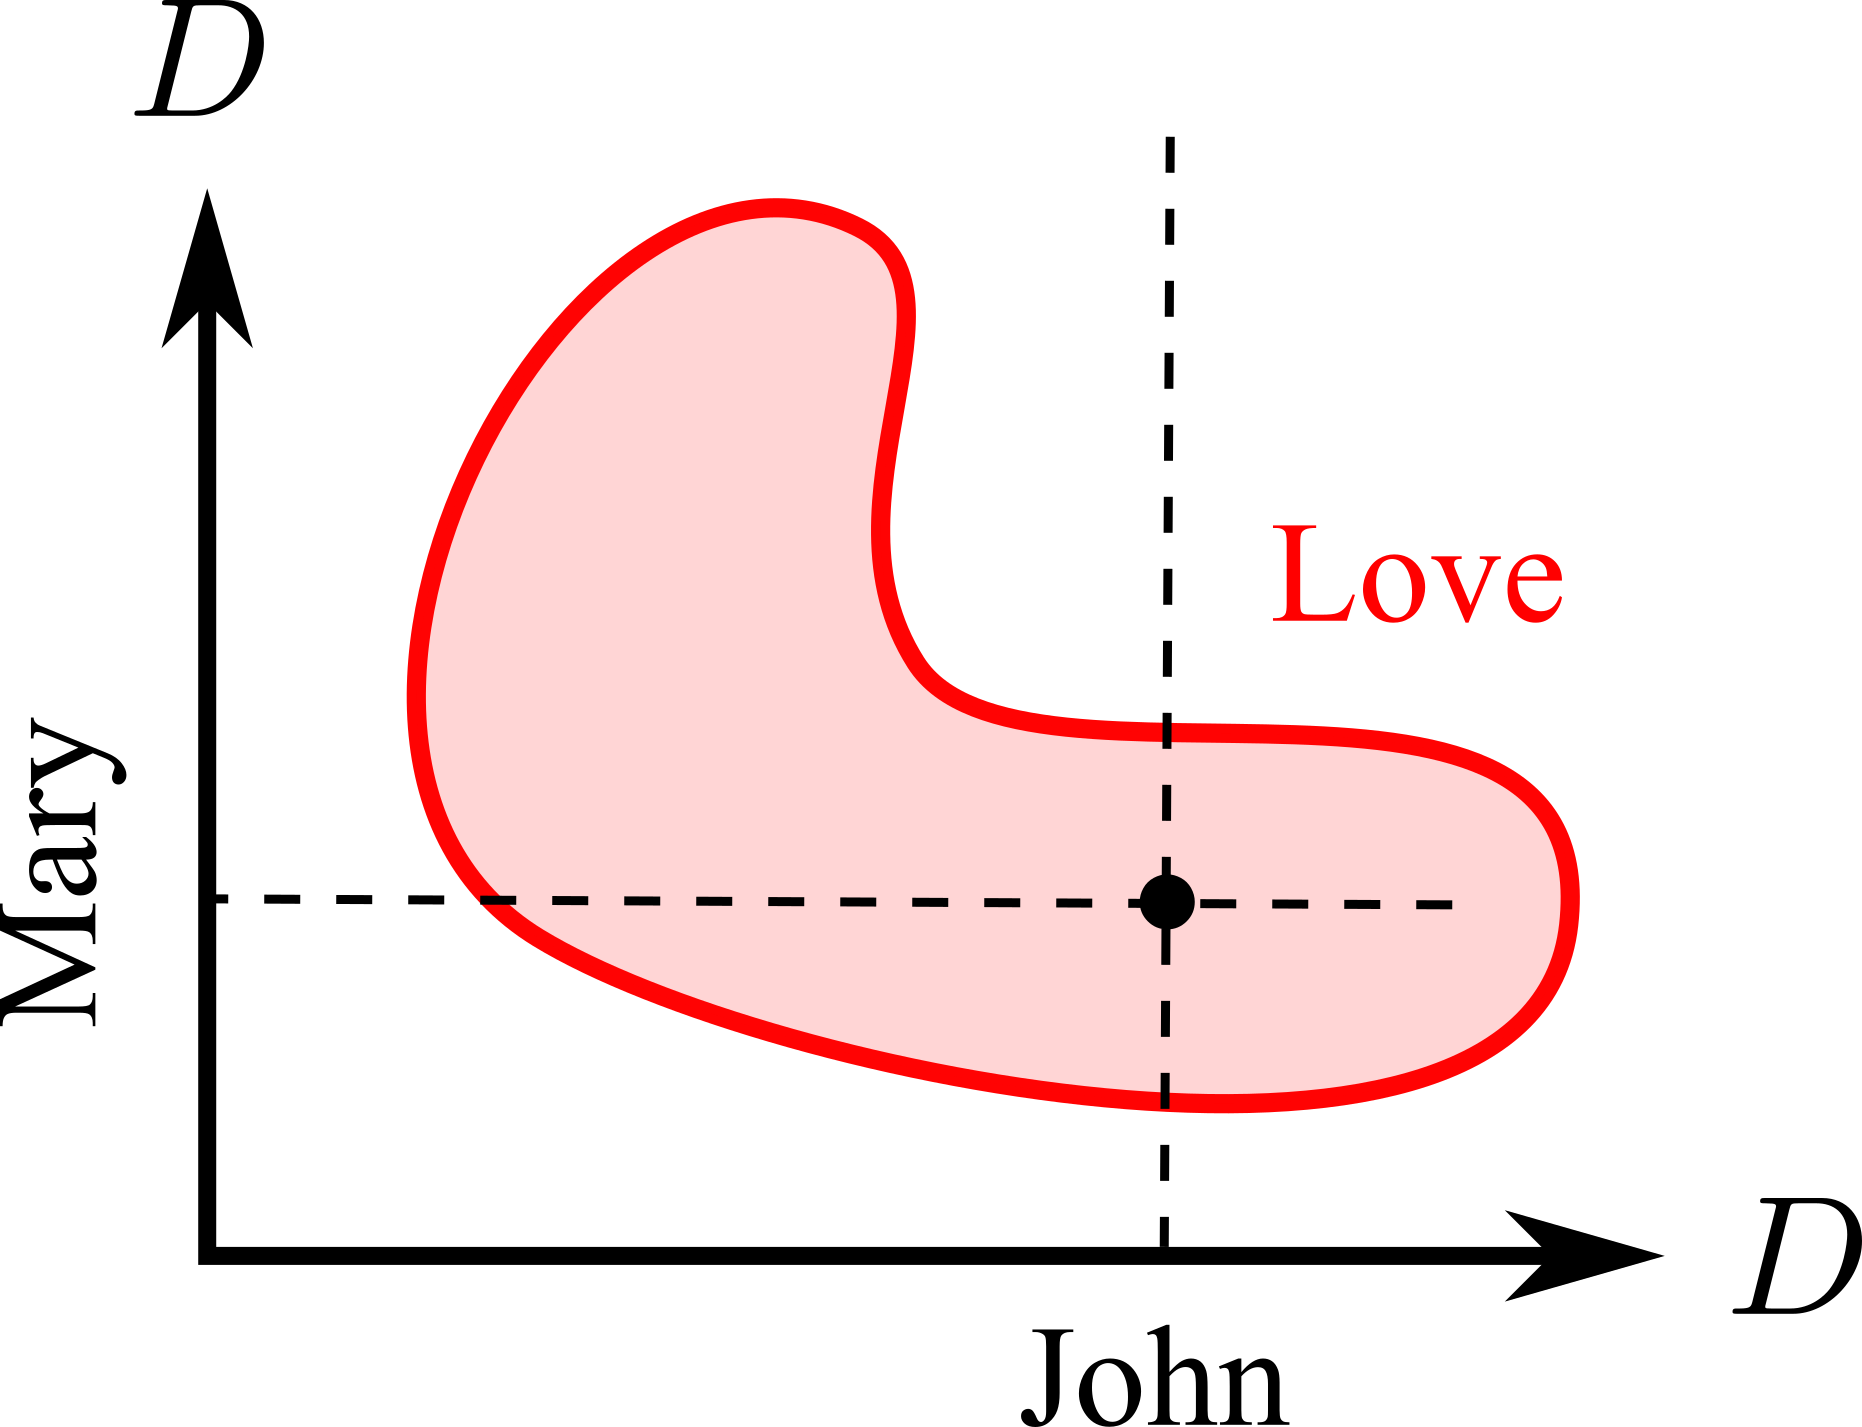
\includegraphics[scale=0.6]{FOL-model-2.png}}} 
\end{equation}

\cc{
对计算系的人来说,更熟识的 model 是以下这种 relation graph 或 \textbf{knowledge graph}: 
}{
For computer science people, you may be more familiar with \textbf{relation graphs} or \textbf{knowledge graphs} such as this one:
}
\begin{equation}
\vcenter{\hbox{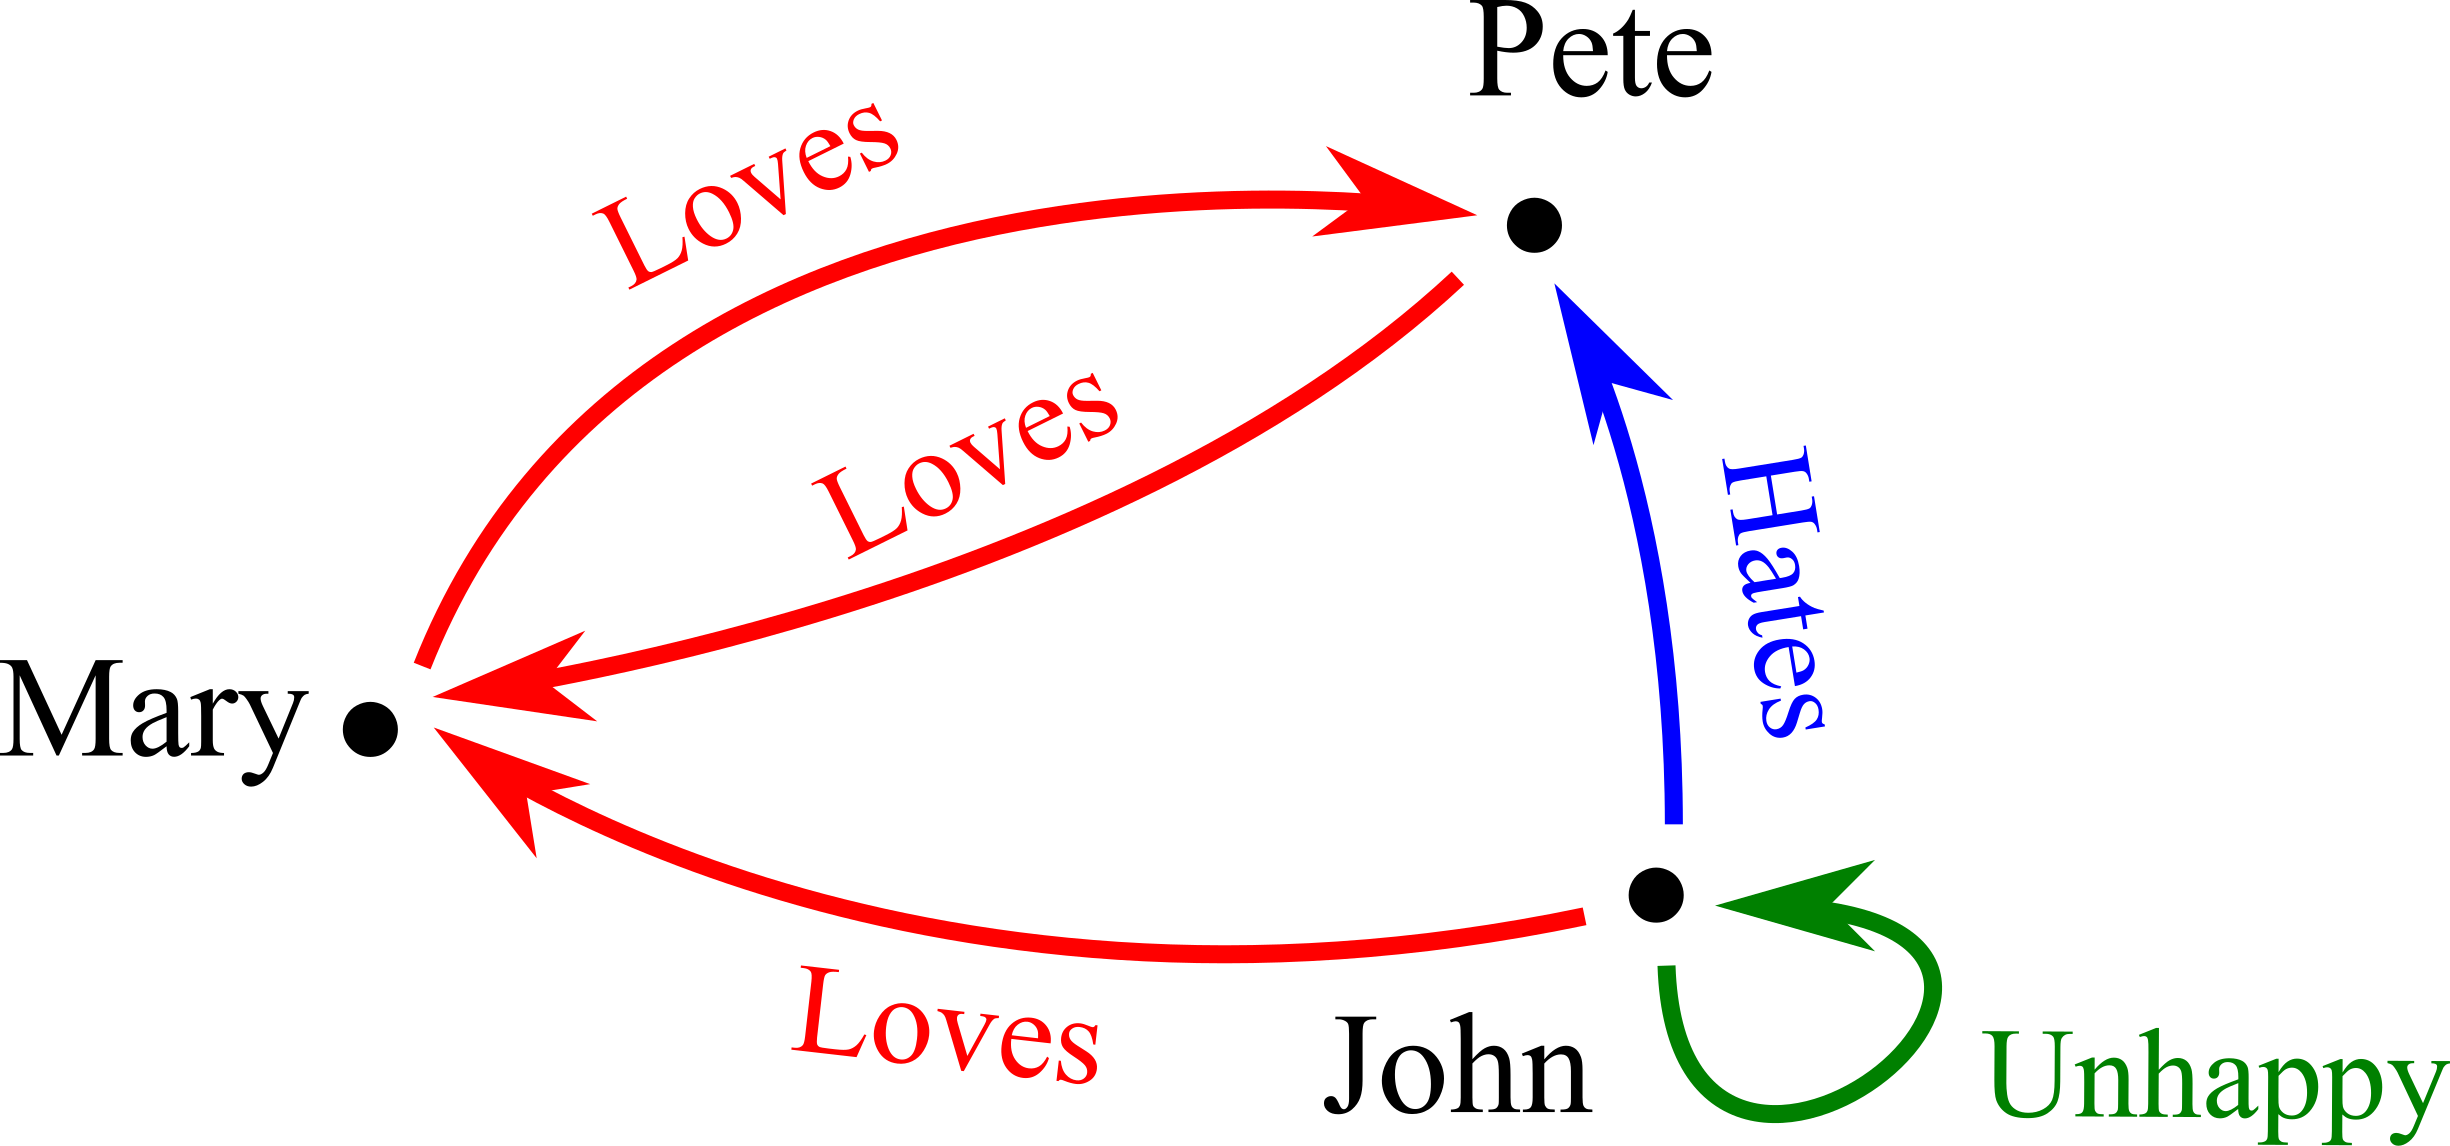
\includegraphics[scale=0.6]{FOL-model-3.png}}} 
\end{equation}
\cc{
这是一个 \textbf{directed multi-graph},或者叫 \textbf{quiver}。  Quiver 是 代数表示论 (representation theory) 中的重要结构。  Quivers 的范畴 $\mathscr{Q}$ 是一个 \textbf{topos}(这会在下文介绍),基本意思是 \uline{它有条件做 first-order logic 的 }\textbf{\uline{模型}}\uline{范畴}。
}{
This is a \textbf{directed multi-graph}, or \textbf{quiver}. Quiver is an important structure in algebraic representation theory.  The category of quivers $\mathscr{Q}$ is a \textbf{topos} (this will be introduced below), basically a topos is \uline{a structure that has the requirements to be a first-order logic }\textbf{\uline{model}}.
}

\cc{
根据 \parencite{Grilliette2017} 的说法,hyper-graph 不是 topos,multi-graph 也不是 topos,但当它们变成 directed 则可以。}{
According to \parencite{Grilliette2017}, a hyper-graph is not a topos, a multi-graph is not a topos, but their \textbf{directed} versions are toposes.
}

Note also that the above graph is somewhat misleading because, strictly speaking, in a topos, \textbf{objects} are \textbf{types} and \textbf{morphisms} are \textbf{terms}.   So ``love'' should be a map from the set of people to itself.  In our graph this is broken down into individual relations.

Perhaps it is most important to understand that the morphism $A \rightarrow B$ in a topos is supposed to mean $A \subset B$ or $A \in B$ in set theory.  For example $\mbox{John} \in \mbox{Men}$ and $(\mbox{John}, \mbox{Mary}) \in \mbox{Love}$.

\cc{以上的 knowledge graph 可以简单地转换成 \textbf{逻辑式子} 的集合:
}{
The above knowledge graph can be easily converted into a collection of \textbf{logic formulas}:}
\footnotesize
\begin{equation}
\begin{array}{l}
	\verb|Loves(John, Mary)| \\
	\verb|Loves(Pete, Mary)| \\
	\verb|Loves(Mary, Pete)| \\
	\verb|Hates(John, Pete)| \\
	\verb|Unhappy(John)|
\end{array}
\label{FOL-model}
\end{equation}
\normalsize
\cc{所以说,\uline{逻辑 与 graph 基本上是 }\textbf{\uline{等价}}\uline{的}。
}{
So, \uline{logic and graphs are basically }\textbf{\uline{equivalent}}.}

\begin{tcolorbox}[breakable, parbox=false, fonttitle=\bfseries, title=Hypergraphs and simplicial complexes]
\cc{如果 graph 的每条 边 可以包含任意个 顶点,则有 \textbf{hyper-graph}。 换句话说,hypergraph 的每条 边 $\in \powerset(V)$,$V$ 是 顶点集。 也可以说,hypergraph 就是 $V$ 的 \textbf{子集系统} (set system)。  对逻辑来说,这好处是: \uline{关系 之上可以有 关系}。  
}{
If an edge of a graph can contain any number of vertices, then we have a \textbf{hyper-graph}. In other words, each edge of the hypergraph $\in \powerset(V)$, $V$ is the vertex set.  It can also be said that the hypergraph is the \textbf{ subset system} of $V$.  For logic, the benefit is that \uline{there can be relations over relations}.}

\cc{Hypergraph 可以一一对应於拓扑学上的 \textbf{simplicial complex},可以研究它的 homology 和 cohomology。 Simplicial complex 也可以和 \textbf{square-free monomial ideals} 一一对应。 Square-free 的意思是 $x_i$ 的指数只可以是 0 或 1。  后者是 \textbf{组合交换代数} (combinatorial commutative algebra) 的研究范围。  暂时我不知道这些关联有没有用,详细可参看 \parencite{Brown2013}, \parencite{Miller2005}。
}{
Hypergraph can 1-1 correspond to topological \textbf{simplicial complexes}, and its homology and cohomology can be studied.  Simplicial complexes can also 1-1 correspond to \textbf{square-free monomial ideals}.  Square-free means that the exponent of $x_i$ can only be 0 or 1.  The latter is the scope of \textbf{combinatorial commutative algebra}.  For the time being, I don't know if these associations are useful.  See \parencite{Brown2013}, \parencite{Miller2005} for details.}
\end{tcolorbox}

\cc{一个逻辑式子的集合叫 logical \textbf{theory}.  一个代数等式的集合叫 \textbf{algebraic theory}.
}{
A collection of logic formulas is called a logic \textbf{theory}.  A collection of algebraic equations is called an \textbf{algebraic theory}.}

\cc{例如可以有以下这个逻辑式子(``失恋则不开心''):
}{
For example, you can have the following logic formula (``unrequited love $\Rightarrow$ unhappy''):}
\begin{equation}
\forall x,y. \; \mbox{Loves}(x,y) \wedge \neg \mbox{Loves}(y,x) \rightarrow \mbox{Unhappy}(x)
\end{equation}
\cc{这个式子含有 universal quantification,所以不是 model 的一部分。 逻辑上来说,只有 \textbf{ground sentences} (没有变量的式子)的集合才可以组成 model,例如 (\ref{FOL-model}) 。 
}{
This formula contains the universal quantification $\forall$, so it is not part of the model.  Logically, only a collection of \textbf{ground sentences} (formulas without variables) can form a model, such as (\ref{FOL-model}) .}

\subsection{\cc{模型空间 的 fractal 结构}{Fractal structure in the model space}}

\cc{Logic \textbf{theory} 中的一个式子 可以导致 model 中出现很多 \textbf{新的} 顶点和连接。 这是 model theory 研究的问题。  某些情况下,模型空间 会出现「无限细分」的 fractal 结构。 
}{
A formula in a logic \textbf{theory} can cause many \textbf{new} vertices and edges to appear in the model.  This is the study of model theory.  In some cases, the model space will have an ``infinitely subdivided'' fractal structure.}

\cc{例如,每一个自然数 $n \in \mathbb{N}$ 都有 它的 successor $S(n)$。 这个函数的存在,导致 model 空间里有一系列 \textbf{无穷} 的顶点:
}{
For example, each natural number $n \in \mathbb{N}$ has its successor $S(n)$.  The existence of this function results in a series of \textbf{infinite} vertices in the model space:}
\begin{equation}
\bullet \quad \bullet \quad \bullet \quad \bullet \quad \bullet \quad \bullet \quad \bullet \quad \bullet \quad \bullet \; .....
\end{equation}
\cc{如果加入这条 \textbf{法则}:
}{
If we add this \textbf{rule}:}
\begin{equation}
\forall n \in \mathbb{N}. \quad S(n) \ge n
\end{equation}
\cc{则立即产生无穷多个关系:
}{
then it immediately generates an infinite number of relations:}
\begin{equation}
\bullet \stackrel{\ge}{\longleftarrow} \bullet \stackrel{\ge}{\longleftarrow} \bullet \stackrel{\ge}{\longleftarrow} \bullet \stackrel{\ge}{\longleftarrow} \bullet \stackrel{\ge}{\longleftarrow} \bullet \stackrel{\ge}{\longleftarrow} \bullet \stackrel{\ge}{\longleftarrow} \bullet \; .....
\end{equation}
\cc{虽然,在 \textbf{日常智能} (common-sense intelligence) 中,似乎比较少出现这种无穷的结构,而更多是 ``shallow'' 的结构。 
}{
Although, in \textbf{common-sense intelligence}, this kind of infinite structures are rare;  usually their structures are ``shallow''.}

\subsection{Partial models in an AI system}

\cc{经典逻辑人工智能 (classical logic-based AI) 的知识表述 是分拆成 \textbf{rules} 和 \textbf{facts} 两部分。 前者是带有 $\forall$ \textbf{变量} 的式子,后者是 ground sentences。  Rules 储存在 $\KB$ 内,facts 储存在 \textbf{working memory} 内。 前者是一个 \textbf{theory},后者可以看成是一些 \textbf{``partial'' models}。  说 partial 的原因是因为它不代表整个 model。  事实上 model 是非常庞大的东西,不可能储存在物理系统中。  人工智能或大脑只能储存 某些 theories 和部分的 models。  人工智能的关键问题是如何找一种良好的 syntax 结构,令 theory 的学习更快、更有效率。 
}{
The knowledge representation of classical logic-based AI is split into two parts: \textbf{rules} and \textbf{facts}. The former are the formulas with $\forall$ \textbf{variables}, the latter are ground sentences.  Rules are stored in $\KB$ and facts are stored in \textbf{working memory}. The former is a \textbf{theory}, the latter can be thought of as some \textbf{``partial'' models}. The reason for saying partial is because it does not represent the entire model. In fact, the model is a huge structure that cannot be stored in any physical system.  AI or the brain can only store certain theories and partial models.  The key issue of AI is how to find a good syntax structure to make theory-learning faster and more efficient.}

\section{\cc{强人工智能的简单表述}{A concise formulation of strong AI}}

\cc{这一节用尽量简练的方式描述强人工智能系统的数学结构,即使没有 AI 背景的数学家也能看懂。
}{
This section describes the mathematical structure of a strong AI system as concisely as possible, so that mathematicians without AI background can understand it.}

\begin{tcolorbox}[breakable, parbox=false, fonttitle=\bfseries, title=Brief review of neural networks]
In short, a neural network is a \textbf{parametrized} function with \textbf{universal approximation} ability.

\cc{重温一下 \textbf{神经网络} 是这样的:
}{
A typical \textbf{neural network} is:}
\begin{eqnarray}
\cc{
\mbox{\footnotesize 每层的} \tikzmark{ww} \mbox{\footnotesize \textbf{权重}矩阵} \quad \quad \mbox{\footnotesize 总层数} \tikzmark{LL} \nonumber \\
\nonumber \\
F(\vec{x}) = \sigmoid(W_1 \tikzmark{wa} \sigmoid(W_2 \tikzmark{wb} ... \sigmoid( W_L \tikzmark{wc} \tikzmark{L} \; \vec{x} )))
\begin{tikzpicture}[overlay,remember picture]
  \draw[-, shorten <=12pt, transform canvas={shift={(-10pt,10pt)}}] (ww.center) to (wa.center);
  \draw[-, shorten <=16pt, transform canvas={shift={(-10pt,10pt)}}] (ww.center) to (wb.center);
  \draw[-, shorten <=28pt, transform canvas={shift={(-10pt,10pt)}}] (ww.center) to (wc.center);
  \draw (LL.center) +(-15pt,-3pt) -- ([shift={(-2pt,6pt)}]L.center);
\end{tikzpicture}
}{
\mbox{\footnotesize \textbf{weights} matrix} \tikzmark{ww} \quad \quad \mbox{\footnotesize total \# layers} \tikzmark{LL} \nonumber \\
\nonumber \\
F(\vec{x}) = \sigmoid(W_1 \tikzmark{wa} \sigmoid(W_2 \tikzmark{wb} ... \sigmoid( W_L \tikzmark{wc} \tikzmark{L} \; \vec{x} )))
\begin{tikzpicture}[overlay,remember picture]
  \draw (ww.center) +(-34pt,-2pt) -- ([shift={(-10pt,10pt)}] wa.center);
  \draw (ww.center) +(-34pt,-2pt) -- ([shift={(-10pt,10pt)}] wb.center);
  \draw (ww.center) +(-34pt,-2pt) -- ([shift={(-10pt,10pt)}] wc.center);
  \draw (LL.center) +(-15pt,-3pt) -- ([shift={(-2pt,6pt)}] L.center);
\end{tikzpicture}
}
\end{eqnarray}
\cc{它的 \textbf{参数} 集合 $\Theta = \{ W_{i, j}^{\ell} \} \in \mathbb{R}^m$,其中 $m$ = \# weights。 
}{
Its set of \textbf{parameters} is $\Theta = \{ W_{i, j}^{\ell} \} \in \mathbb{R}^m$, where $m$ = \# weights.}

\cc{\textbf{机器学习} 的目的是 \uline{寻找 optimal $\Theta$ subject to an objective function}.  换句话说,机器学习 = \textbf{optimization},这是应用数学的最基本问题之一。
}{
The purpose of \textbf{machine learning} is to \uline{find the optimal $\Theta^*$ subject to an objective function}.  In other words, machine learning = \textbf{optimization}, which is one of the most basic problems in applied mathematics.}

\cc{训练时,给定一组 data points($F$ 是神经网络):
}{
During training, it is given a set of data points ($F$ is a neural network):}
\begin{equation}
\label{NN-training}
\boxed{\mbox{training examples}} \quad
e \stackrel{F}{\longrightarrow} a
\quad \boxed{\mbox{answers}} 
\end{equation}
\cc{每个答案的误差是 $\epsilon$,目标函数 $J$ 是很多次 iterations 的误差之和。
}{
The error for each answer is $\epsilon$, and the objective function $J$ is the sum of the errors over many iterations.}
% \begin{equation}
% J = \sum_t \epsilon \; ( e, a, \Theta )
% \end{equation}
\cc{我们想令 $J$ 最优化,方法是计算 $J$ 对于 $\Theta$ 的梯度 (gradient):
}{
We want to optimize $J$ by calculating the gradient of $J$ w.r.t. $\Theta$:}
\begin{equation}
\nabla_{\Theta} J := \frac{\partial J}{\partial \Theta}
\end{equation}
\cc{当然这就是著名的 back-propagation 算法,其实即 gradient descent。
}{
Of course, this is the famous \textbf{back-propagation} algorithm, which is actually gradient descent.}

If the sigmoid function $\sigmoid$ is replaced by a polynomial function $\NewSym[1.0]{../polynomial.png} \,$ , the overall network function would be a composite polynomial whose \textbf{degree} is the product of the degrees of every layer.  In other words, the total degree grows \textbf{exponentially} as \#(layers) grows.  As the polynomial degree is the number of \textbf{zero-crossings}, it can be regarded as the number of possible \textbf{classifications} discernable by the network.  For example, a quintic polynomial can distinguish up to 5 classes:
\begin{equation}
\vcenter{\hbox{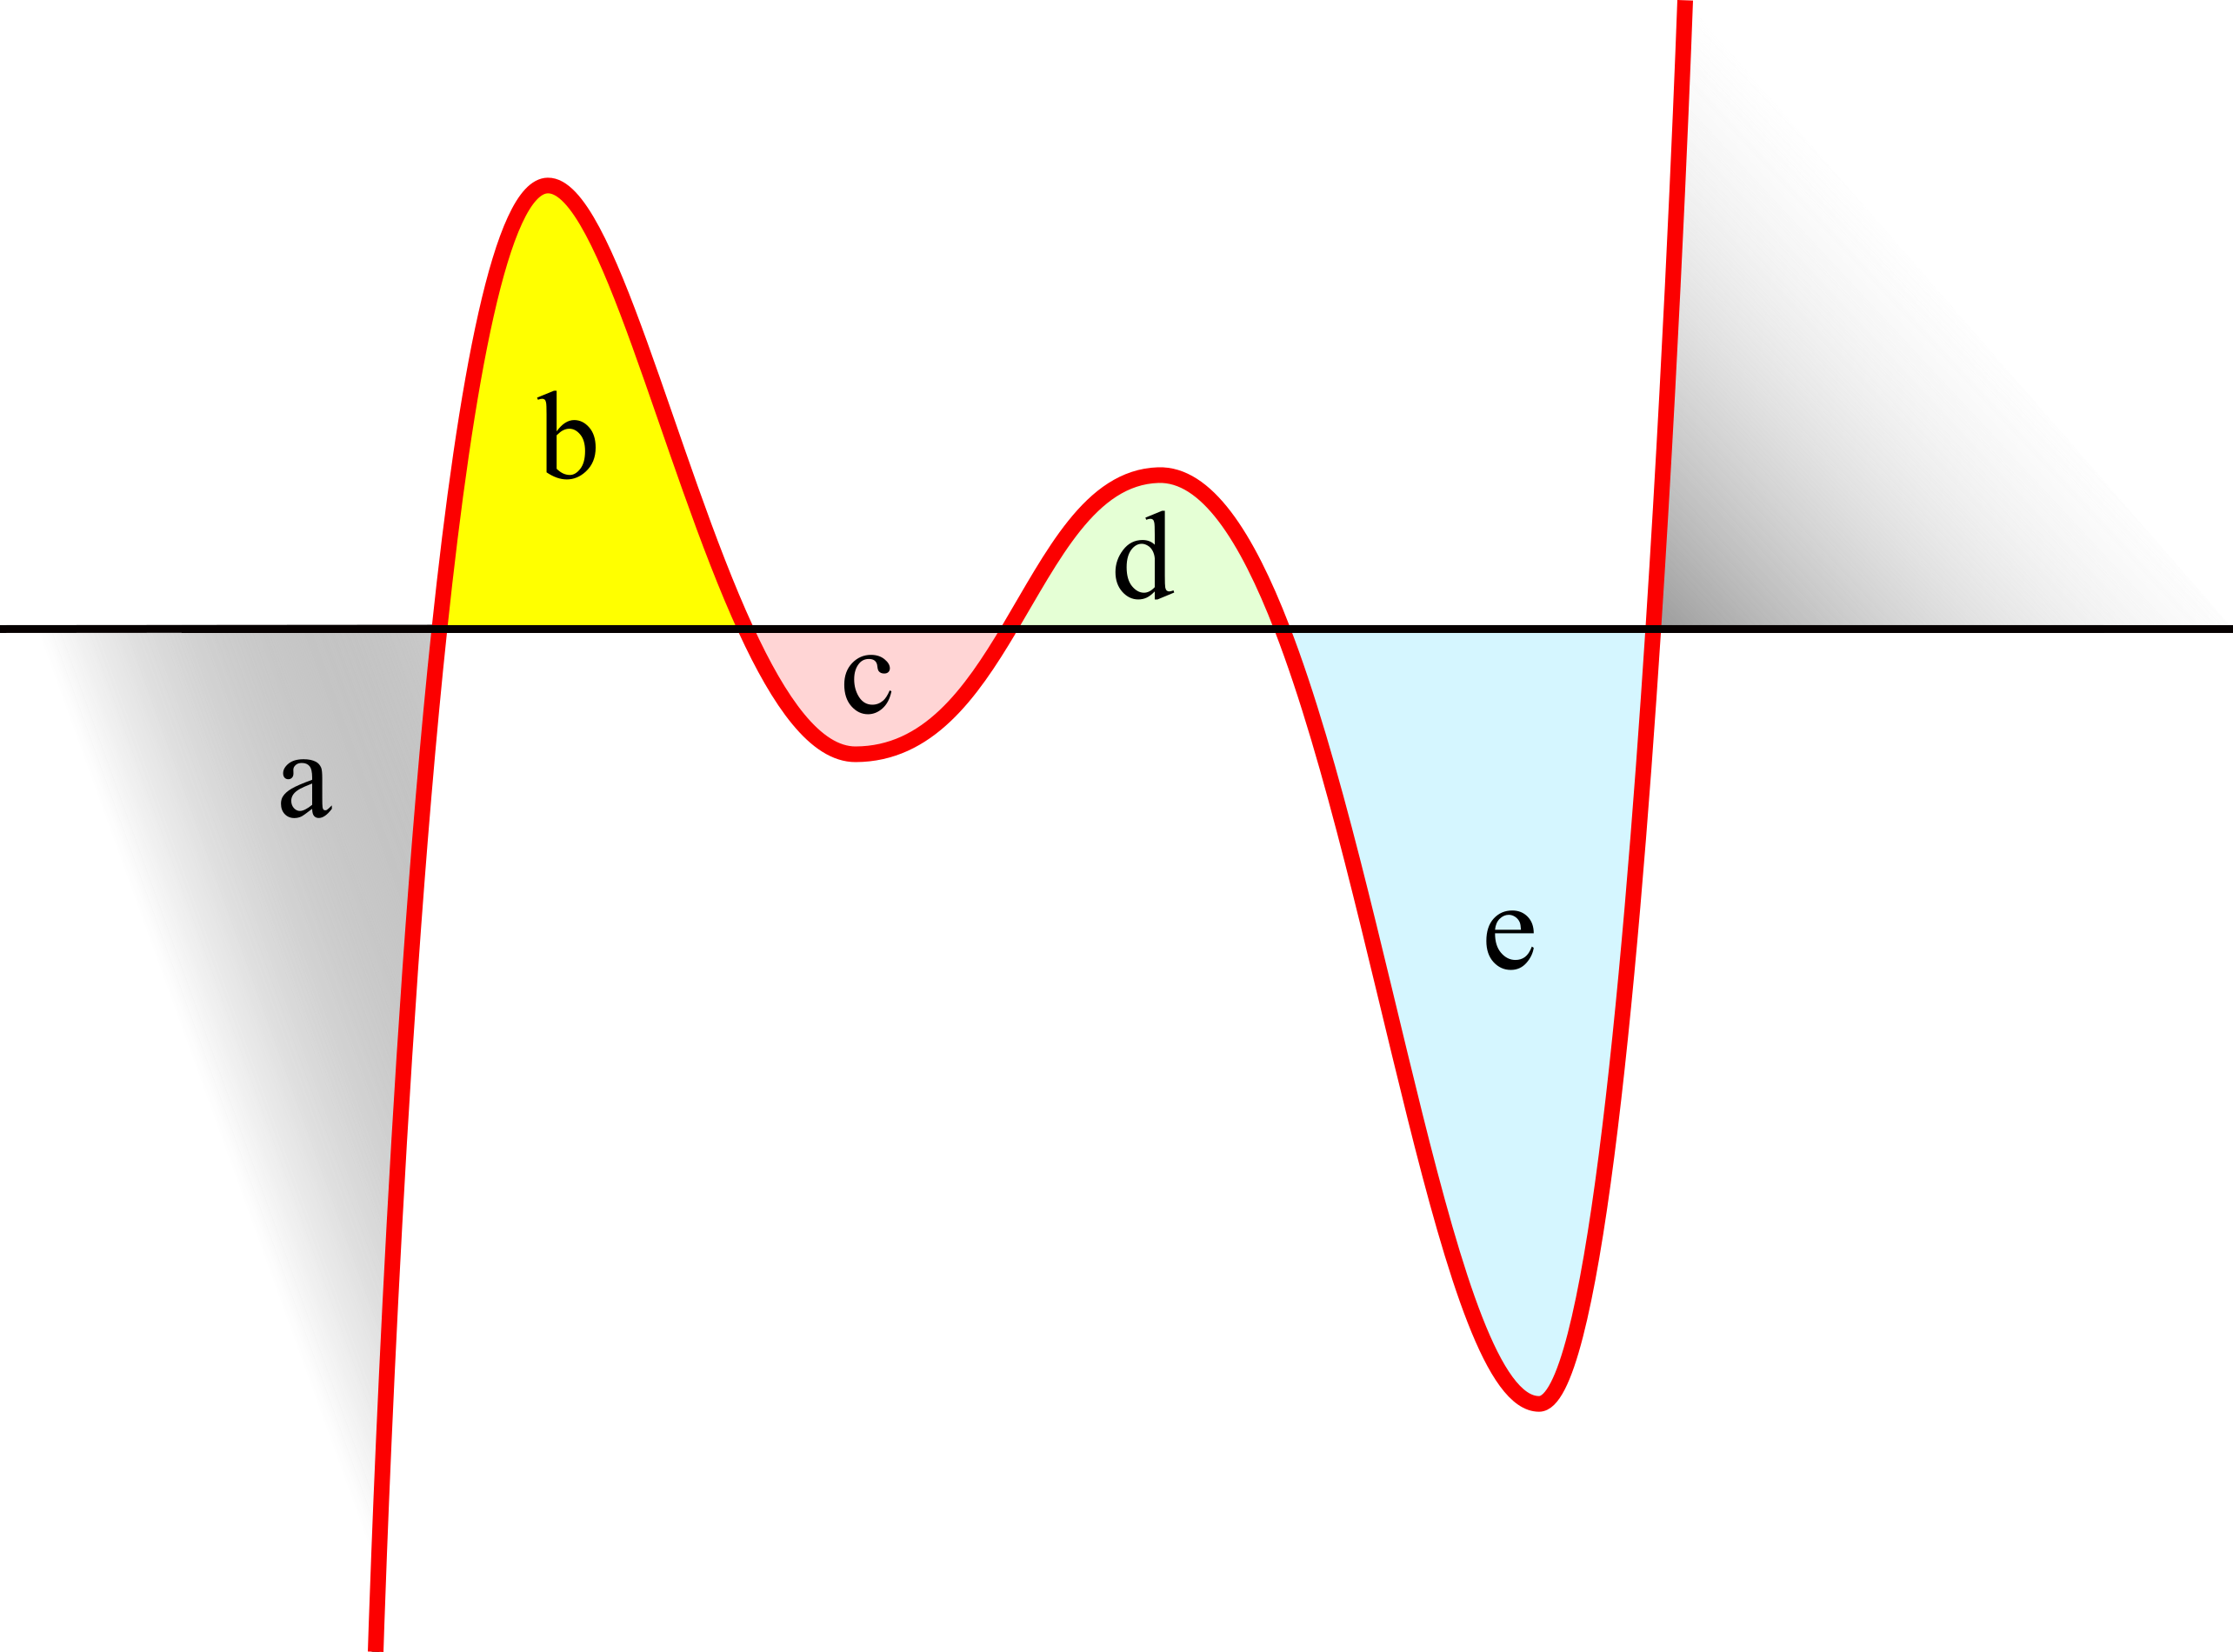
\includegraphics[scale=0.6]{zero-crossings.png}}}
\end{equation}
In other words, \uline{the classifying power of NN increases exponentially as \#(layers)}.  

Consider an NN whose inputs and outputs are \textbf{binarized} and of the same size, ie, it maps $\{0,1\}^n \rightarrow \{0,1\}^n$.  The number of such distinct discrete functions is $(2^n)^{2^n} = 2^{n 2^n}$, this number is \textbf{doubly exponential} in $n$, and is so large that in practice it could be regarded as $\infty$.  Yet an NN is able to approximate this function space using $L \cdot n^2$ weights.  The \textbf{hierarchical} organization of weights is what gives the NN its \textit{``unreasonable effectiveness''}.
\end{tcolorbox}

\cc{
\uline{强人工智能 的樽颈问题 是\textbf{学习算法}的速度。}}{
\uline{The bottleneck of strong AI is in the \textbf{learning algorithm} being too slow}.
}

\cc{AI 学习算法的特点是 \uline{需要在 }\textbf{\uline{ 逻辑式子}}\uline{ 上进行最优化}:
}{
What is special about an AI learning algorithm is that \uline{it performs optimization over }\textbf{\uline{ logic formulas}} instead of the usual $\mathbb{R}^n$:}
\begin{tcolorbox}[ams align, colback=yellow, colframe=white]
\cc{
\mbox{从 } \mbox{ optimization over $\mathbb{R}$} && \mbox{ 过渡到 } & \mbox{ optimization over $\mathscr{L}$} \nonumber\\
}{
& \mbox{Passage from optimization over $\mathbb{R}$} \mbox{ to optimization over $\mathscr{L}$} \nonumber\\
}
& \quad \quad \quad \quad \Theta \in \mathbb{R}^n \quad \rightsquigarrow \quad \Theta \in \mathscr{L}
\end{tcolorbox}
\cc{其中 $\mathscr{L}$ 是某种 (例如一阶谓词)\textbf{逻辑语法},$\Theta$ 是一个逻辑式子的集合。 这最优化问题的解 $\Theta^*$ 是一个 optimal logic theory。
}{
Where $\mathscr{L}$ is some kind of (\textit{eg} first-order predicate) \textbf{logical syntax}, and $\Theta$ is a set of logic formulas.  The solution to this optimization problem $\Theta^*$ is an optimal logic theory.}

\cc{系统的 top-level architecture 是 强化学习,亦即 dynamic programming,是 optimization 的一个特例,也可以叫 control theory,它控制的\textbf{系统}是:
}{
The top-level architecture of the system is reinforcement learning, a.k.a. dynamic programming. It is a special case of optimization. It can also be called control theory. The \textbf{system} it controls is:}
\begin{equation}
\vec{x}_{t+1} = \vec{f}( \vec{x}_t, \vec{u}_t )
\end{equation}
\cc{$\vec{x}$ 是系统的\textbf{状态},$\vec{u}$ 叫 control 或 action。 在 AI 里,$\vec{x}$ 是「思维空间」中的\textbf{位置},$\vec{u}$ 是「思考」的 steps。 我们希望控制 $\vec{u}$,令系统在\uline{长时间的运行中},收到的\textbf{奖励}达到最大值: 
}{
$\vec{x}$ is the system's \textbf{state}, $\vec{u}$ is called the \textbf{control} or action. In AI, $\vec{x}$ is the \textbf{position} in ``cognitive space'', and $\vec{u}$ is the ``thinking'' steps. We want to control $\vec{u}$ so that the system reaches the maximum value of \textbf{rewards} \uline{over the long run}:}
\begin{equation}
\boxed{\mbox{total rewards}} \quad J = \sum_t L(\vec{x}) = \int L dt
\end{equation}
\cc{$L \in \mathbb{R}$ 是在 $\vec{x}$ 位置得到的\textbf{瞬时奖励},基於历史上分析力学的原因,$L$ 也叫作 \textbf{Lagrangian},单位是能量(但正负号改变,后者量度的是惩罚),但注意这里的 $\vec{x}$ 是「思维空间」,不同於物理空间。 我附带写上微分形式,以便於记忆。
}{
where $L \in \mathbb{R}$ is the \textbf{instantaneous reward} at position $\vec{x}$.  Due to historical reasons (from analytic mechanics), $L$ is called the \textbf{Lagrangian}, its unit is energy (but the sign is reversed, now it measures the penalty), and note that $\vec{x}$ is in ``cognitive space'' which is not the same as physical space.  I prefer to write the differential version as it is easier to remember.}

\cc{系统的运行如下:
}{
The system operates as follows:}
\begin{equation}
\vcenter{\hbox{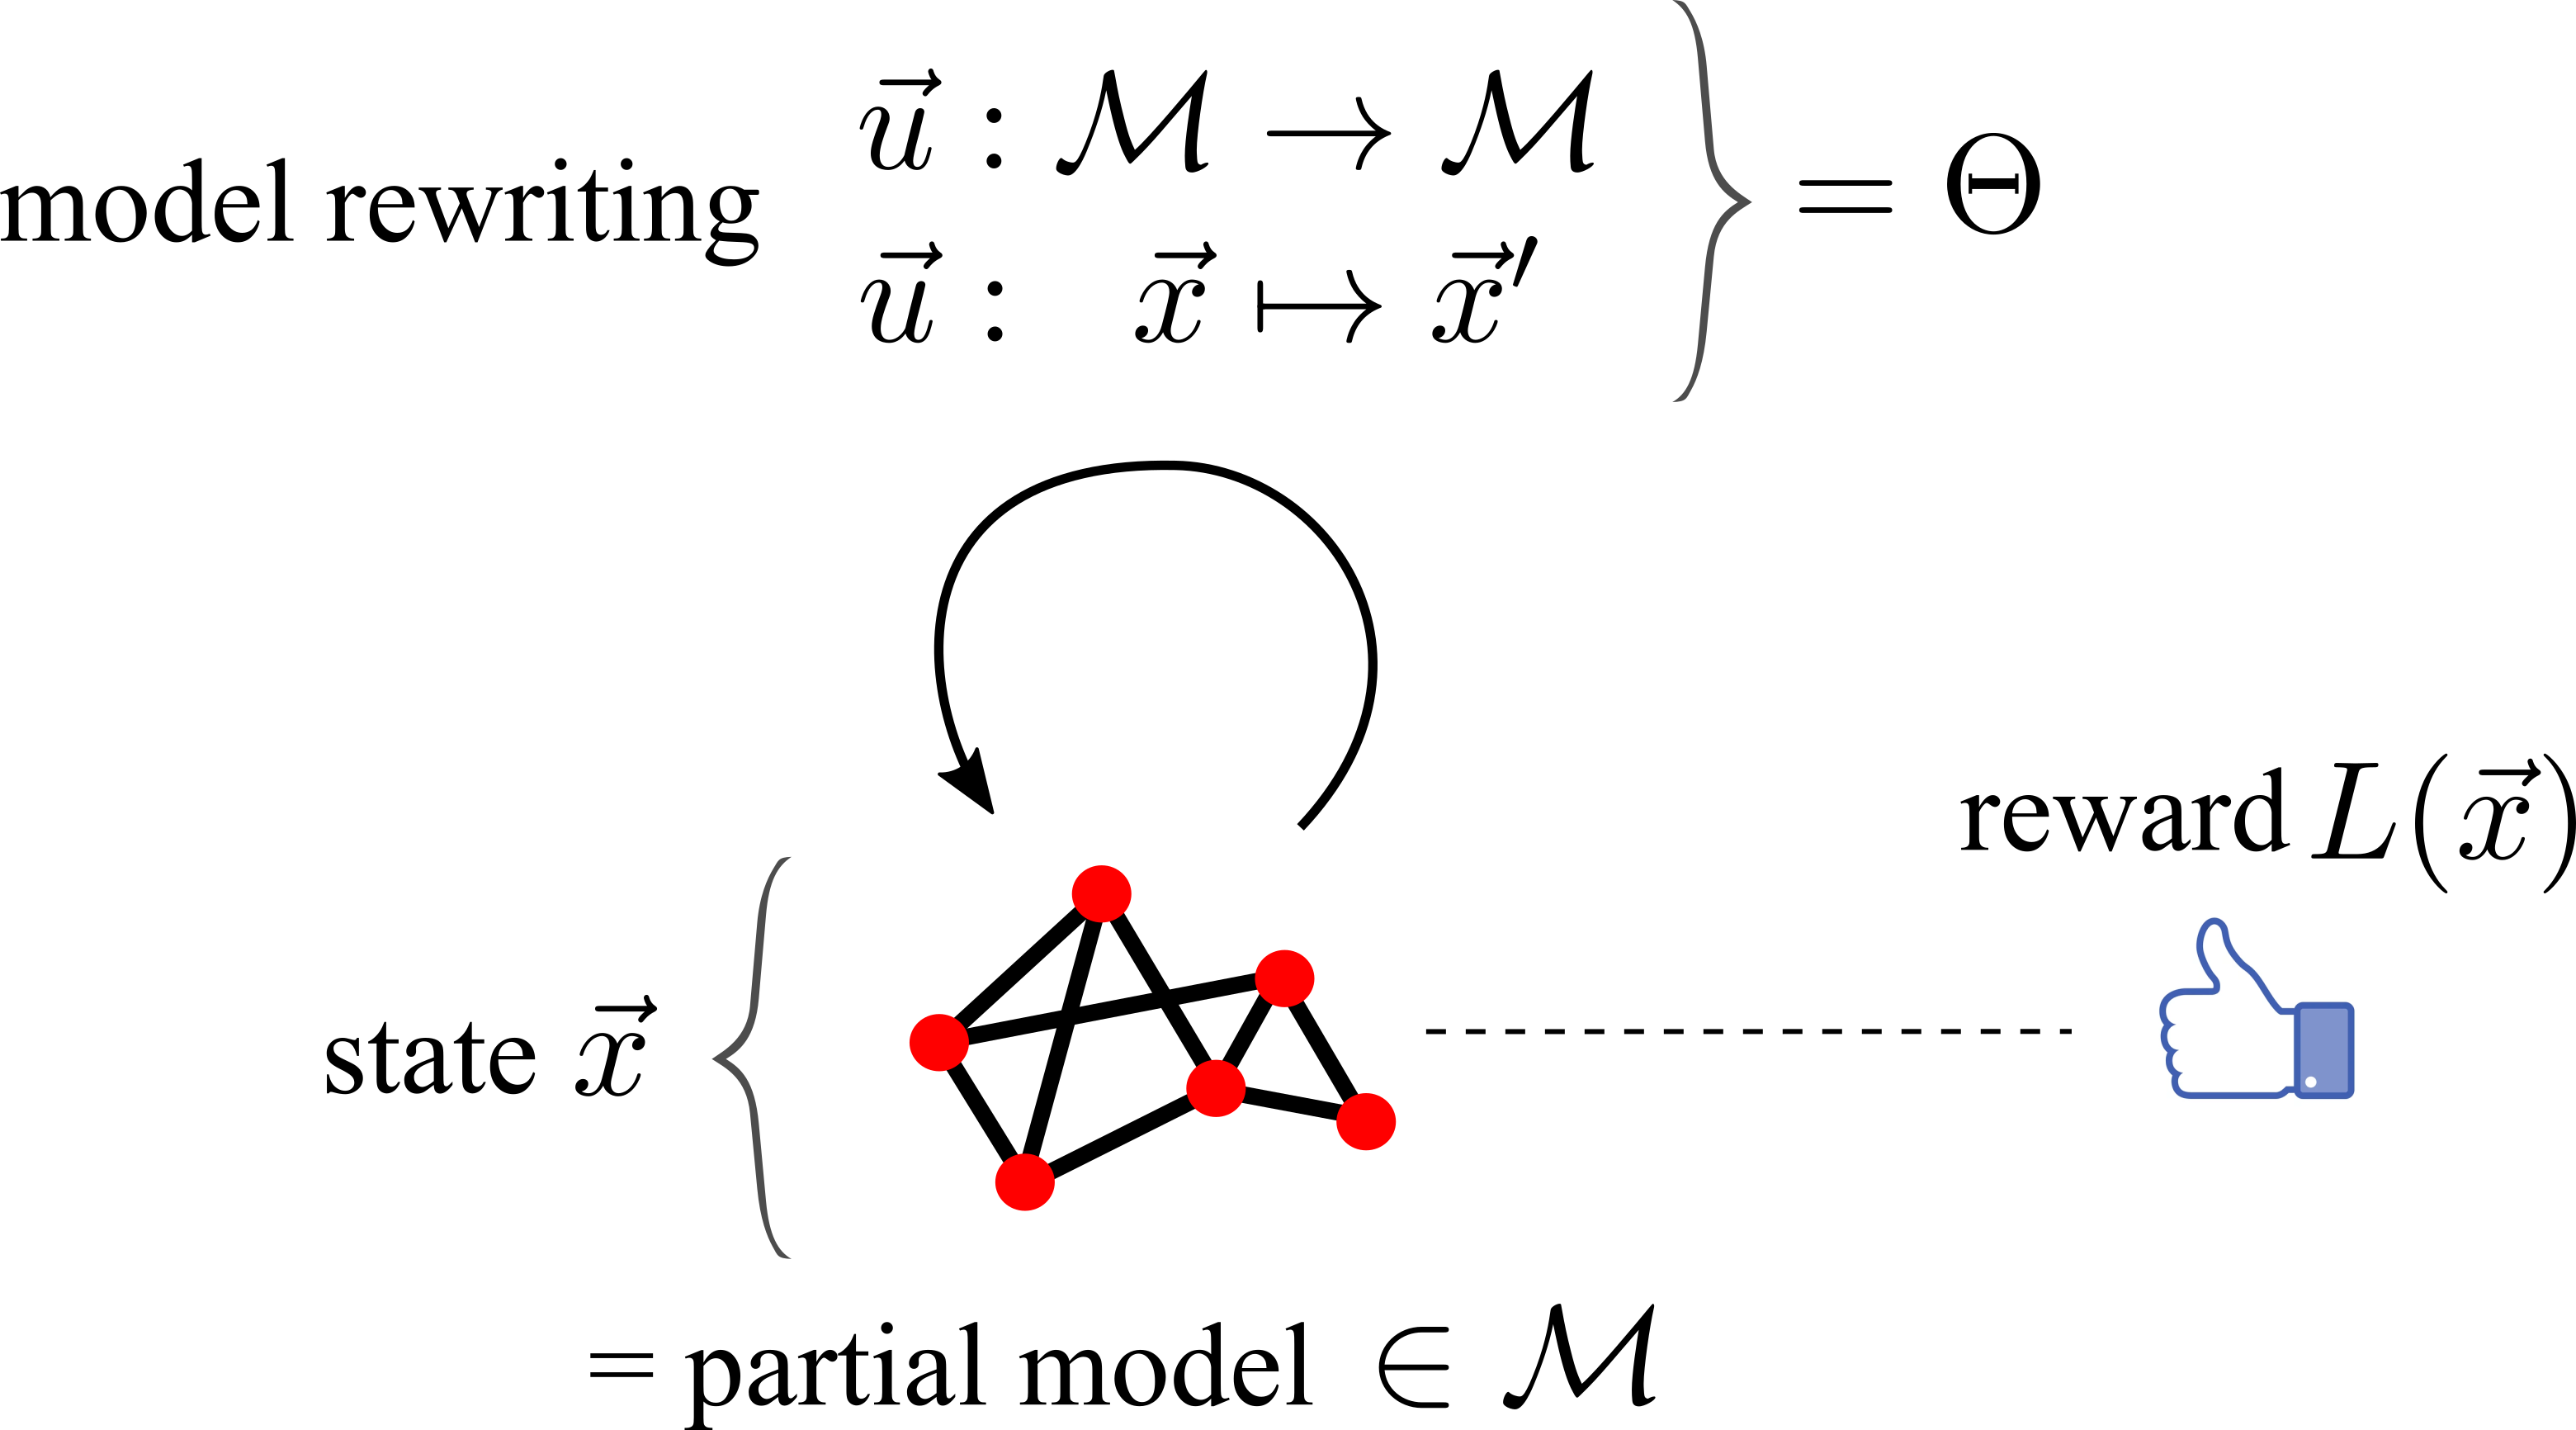
\includegraphics[scale=0.7]{abstract-dynamic-programming.png}}}
\end{equation}
% $\vec{x}$ 的某些部分用作\textbf{输出},经由它得到奖励。 
\cc{$\vec{u}$ 和 $\vec{f}$ 重合,作用是将 $\vec{x}$ \textbf{重写}:
}{
$\vec{u}$ and $\vec{f}$ coincide, its function is to \textbf{rewrite} $\vec{x}$:}
\begin{equation}
\vec{f}(\vec{x},\vec{u}) \equiv \vec{u}(\vec{x})
\end{equation}
\cc{For example, the logic rule ```失恋 $\Rightarrow$ 不开心'' performs the rewriting of the following sub-graph:
}{
For example, the logic rule ```失恋 $\Rightarrow$ 不开心'' performs the rewriting of the following sub-graph:}
\begin{equation}
\vcenter{\hbox{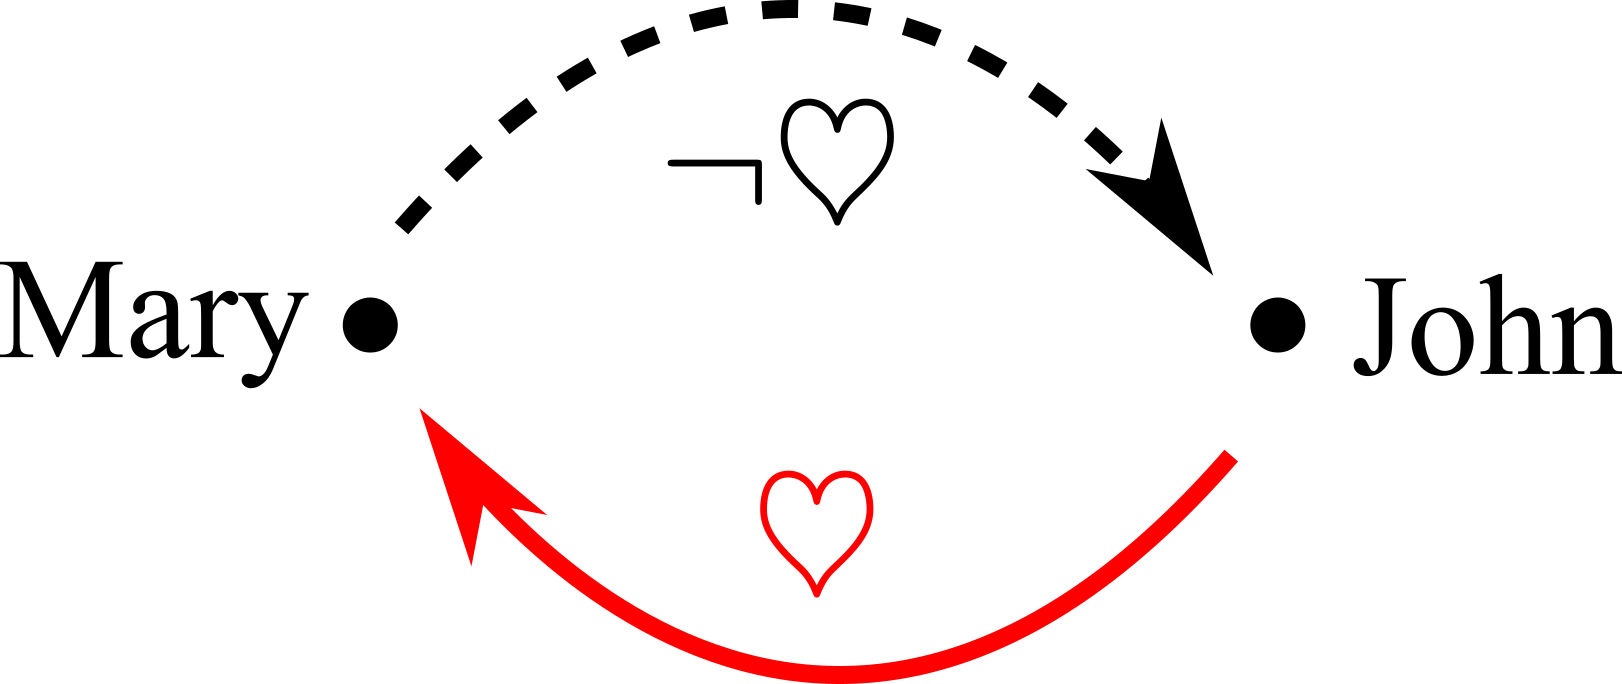
\includegraphics[scale=0.6]{heartbreak-precond.png}}}
\quad \mapsto \quad
\vcenter{\hbox{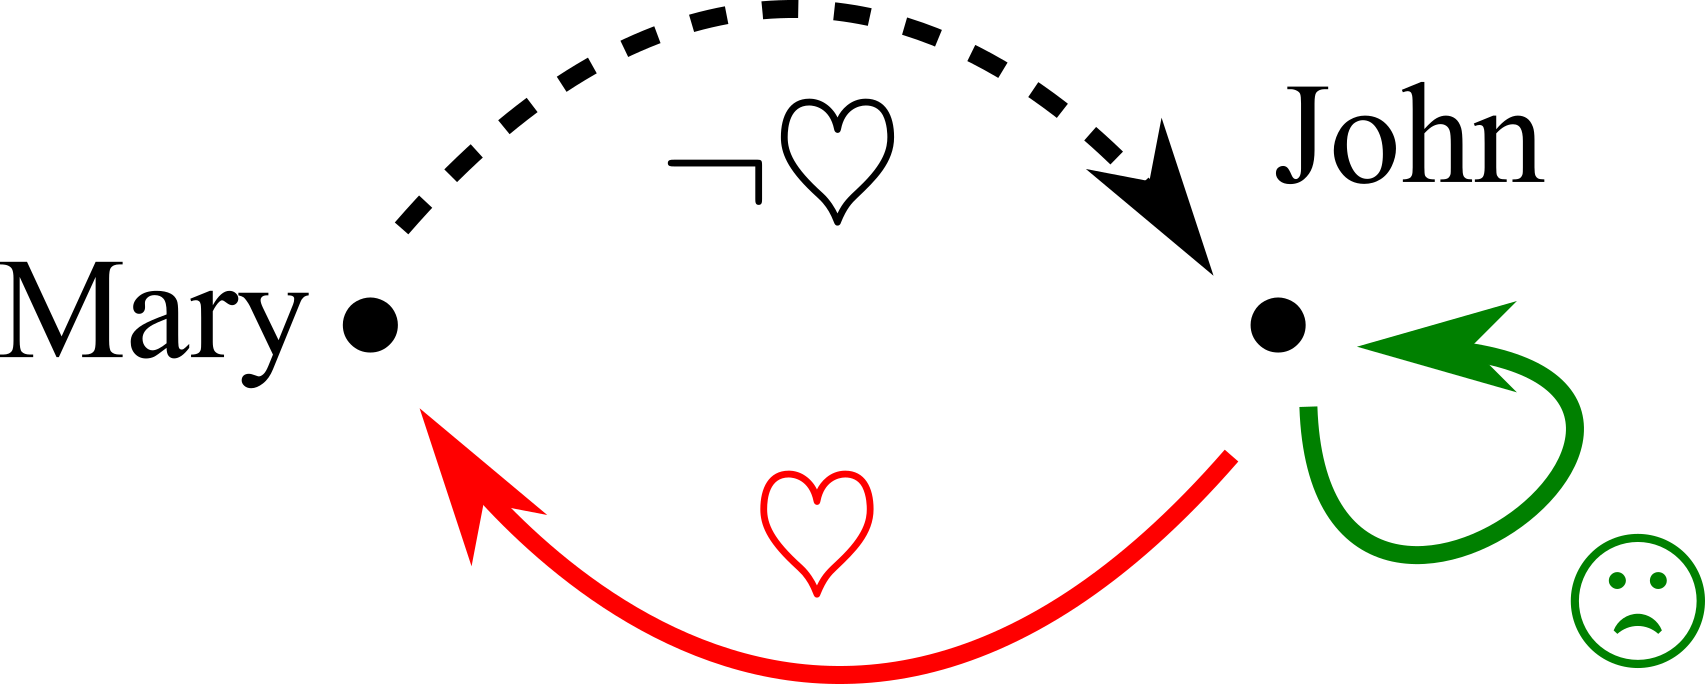
\includegraphics[scale=0.6]{heartbreak-postcond.png}}}
\end{equation}
\cc{This is the \textbf{state transition} $\vec{u}: \vec{x} \mapsto \vec{x}'$, which can also be regarded as the \textbf{logical inference} $\vec{u}: \vec{v} \vdash \vec{x}'$, where $\vec{u}$ is the rewriting function or logic rule.
}{
This is the \textbf{state transition} $\vec{u}: \vec{x} \mapsto \vec{x}'$, which can also be regarded as the \textbf{logical inference} $\vec{u}: \vec{v} \vdash \vec{x}'$, where $\vec{u}$ is the rewriting function or logic rule.}

\cc{Optimization of $J$ 作用在 $\Theta$(亦即 $\vec{u}$)之上。  注意 $\vec{u} \in$ 某种 function space or 逻辑式子,这和传统的 optimization over $\mathbb{R}$ 很不同。 
}{
Optimization of $J$ acts over $\Theta$ (ie $\vec{u}$). Note that $\vec{u}$ belongs in a function space or the space of logic formulas, which is very different from the traditional optimization over $\mathbb{R}$.}

\footnotesize
\cc{在经典 AI 中,$\vec{u}(\vec{x}) = \vec{f}(\vec{x})$ 的作用相当於 deduction $\vec{x} \vdash \vec{x}'$,或者叫 forward-chaining(向前推导出一些逻辑结论)。  在经典 AI 中这工作由 \textbf{逻辑引擎} 负责,它包含 \textbf{unification} (= rule matching) 和 \textbf{resolution} (= proof search) 两个算法。  在我们的框架中 看不到这些运作,因为它们被包含在 $\vec{u}$ 或 $\vec{f}$ 之内。 
}{
In classic AI, $\vec{u}(\vec{x}) = \vec{f}(\vec{x})$ is equivalent to the deduction $\vec{x} \vdash \vec{x} '$, also known as \textbf{forward-chaining} (deduce logical conclusions).  In classic AI this job is handled by an \textbf{inference engine}, which consists of 2 algorithms: \textbf{unification} (= rule matching) and \textbf{resolution} (= proof search). These operations are not visible in our framework as they are absorbed into $\vec{u}$ or $\vec{f}$.}
\normalsize

%训练的过程类似 (\ref{NN-training}):
%\begin{equation}
%\boxed{\mbox{training examples}} \quad
%e \sststile{}{\Theta} a
%\quad \boxed{\mbox{answers}} 
%\end{equation}
%但现在 $\vdash$ 是根据 $\Theta$ 的 \textbf{逻辑推导},$e$ 和 $a$ 是逻辑式子的集合。 给定一些前提,可以推出很多结论,其中有些得到奖励或惩罚。 % 在 \textbf{强化学习} (reinforcement learning,亦即 dynamtic programming) 的框架下,训练是根据 \textbf{奖励} 而不是 \textbf{误差},和上面略有不同。 

\subsection{Hamilton-Jacobi-Bellman equation}

\cc{对应用数学方面的专家们来说,以下的理论是颇为 standard 的。  它纯粹设定 AI 系统在强化学习的框架下,除此以外没有其他实质内容。 

分析力学中 Hamiltonian 的定义是:
}{
For experts in applied mathematics, the following theory is quite standard.  It merely sets up the AI system under the framework of reinforcement learning, which otherwise has no substantial content.

The definition of Hamiltonian in analytical mechanics is:}
\begin{equation}
H = L + \frac{\partial J}{\partial \vec{x}} \vec{f}
\end{equation}
\cc{类似地,\textbf{离散}系统的 Hamiltonian 可以定义为:
}{
Similarly, the Hamiltonian of the \textbf{discrete} system can be defined as:}
\begin{equation}
H = L + J ( \vec{f}(\vec{x}) )
\end{equation}
\cc{Pontryagin\footnote{Lev Pontryagin (1908-1988) Soviet mathematician. Blind since the age of 14, he made major discoveries in a number of fields including algebraic topology and differential topology.} 的 \textbf{极小值原理} 给出最优解的条件是:
}{
Pontryagin\footnote{Lev Pontryagin (1908-1988) Soviet mathematician. Blind since the age of 14, he made major discoveries in a number of fields including algebraic topology and differential topology.} 's \textbf{maximum principle} gives the condition for the optimal solution:}
\begin{equation}
\label{Pontryagin-max-principle}
H^* = \inf_u H \quad \mbox{or} \quad \nabla_{\vec{u}} H^* := \frac{\partial H^*}{\partial \vec{u}} = 0
\end{equation}
\cc{可以定义一个作用在 $J$ 上的算子 $T$:
}{
We can define an operator $T$ that acts on $J$:}
\begin{equation}
T J := \inf_u H
\end{equation}
\cc{则 Bellman's optimality condition 可以表示为以下的 fixed-point 形式 \parencite{Bertsekas2013}:
}{
Then Bellman's optimality condition can be expressed as the following fixed-point equation \parencite{Bertsekas2013}:}
\begin{equation}
J^* = T J^*
\end{equation}
\cc{据说 Hamilton-Jacobi 方法导致解 偏微分方程,不是特别有效,实践中更有用的是 Pontryagin 极小值原理。
}{
It is said that the Hamilton-Jacobi method leads to the solving of partial differential equations, which is not particularly efficient.  In practice, the Pontryagin minimum principle is more useful.}

\cc{在 (\ref{Pontryagin-max-principle}) 式中有梯度 $\nabla_{\vec{u}}$,所以如果能对 $\vec{u}$ 求导数是会很有用的。  如果问题是 continuous optimization,可以用 non-smooth analysis,其最低要求是 domain 上有 norm (\textit{ie}, Hilbert space or Banach space),则可以用 proximal gradient 等方法。 
}{
There is a gradient $\nabla_{\vec{u}}$ in (\ref{Pontryagin-max-principle}), so it would be useful to find a derivative for $\vec{u}$. If the problem is continuous optimization, one can use non-smooth analysis. The minimum requirement is that there is a norm (\textit{ie}, Hilbert space or Banach space) in the domain, then we can employ techniques such as proximal gradient.}

One question is: why hasn't the keyword ``\textbf{symplectic}'' appeared in current AI literature on reinforcement learning, while all existing techniques are \textbf{statistical} in nature?  I suspect that it may be due to either: 1) the time-step being discrete; or 2) the dimensionality of the state space being too high (though this dimensionality may not be \textit{intrinsic} to the problem, \textit{ie}, it may be possible to embed into lower dimensions).

% \cc{关键问题是: $\Theta$ 属於的 domain 不是传统的 $\mathbb{R}^n$。
% }{
% The key issue is: $\Theta$ belongs to a domain different from the traditional $\mathbb{R}^n$.}

\section{Plan 0: geometric models}

\begin{tcolorbox}[ams equation, colback=yellow, colframe=white]
\cc{
\mbox{一阶逻辑语法 $\mathscr{L}$ 不是必需的,只需某种将 model \textbf{改写} 的能力}}{
\begin{aligned}
\mbox{first-order syntax $\mathscr{L}$ is unnecessary; } \\
\mbox{we only need the ability to \textbf{rewrite} models}
\end{aligned}
}
%\uline{一阶逻辑语法 $\mathscr{L}$ 不是必需的,只需要某种将 model }\textbf{\uline{改写}}\uline{的能力}。 
\end{tcolorbox}
\cc{可以有很多不同的变种,例如:
}{
There can be many variations on this theme, for example:}
\begin{equation}
\begin{tikzcd}[column sep = large]
\cc{
\mbox{逻辑语法 } \; \mathscr{L} \arrow[d] \\}{
\mbox{logical syntax } \; \mathscr{L} \arrow[d] \\
}
\mbox{partial model } \mathscr{M}
\end{tikzcd}
\approx
\begin{tikzcd}[column sep = large]
\mbox{graph re-writer} \arrow[d] \\
\mbox{graph model}
\end{tikzcd}
\end{equation}

Consider a kind of what I call \textbf{geometric models}, as typically exemplified by Venn diagrams:
\begin{equation}
P(x) \wedge Q(x) \quad \cong \quad
\vcenter{\hbox{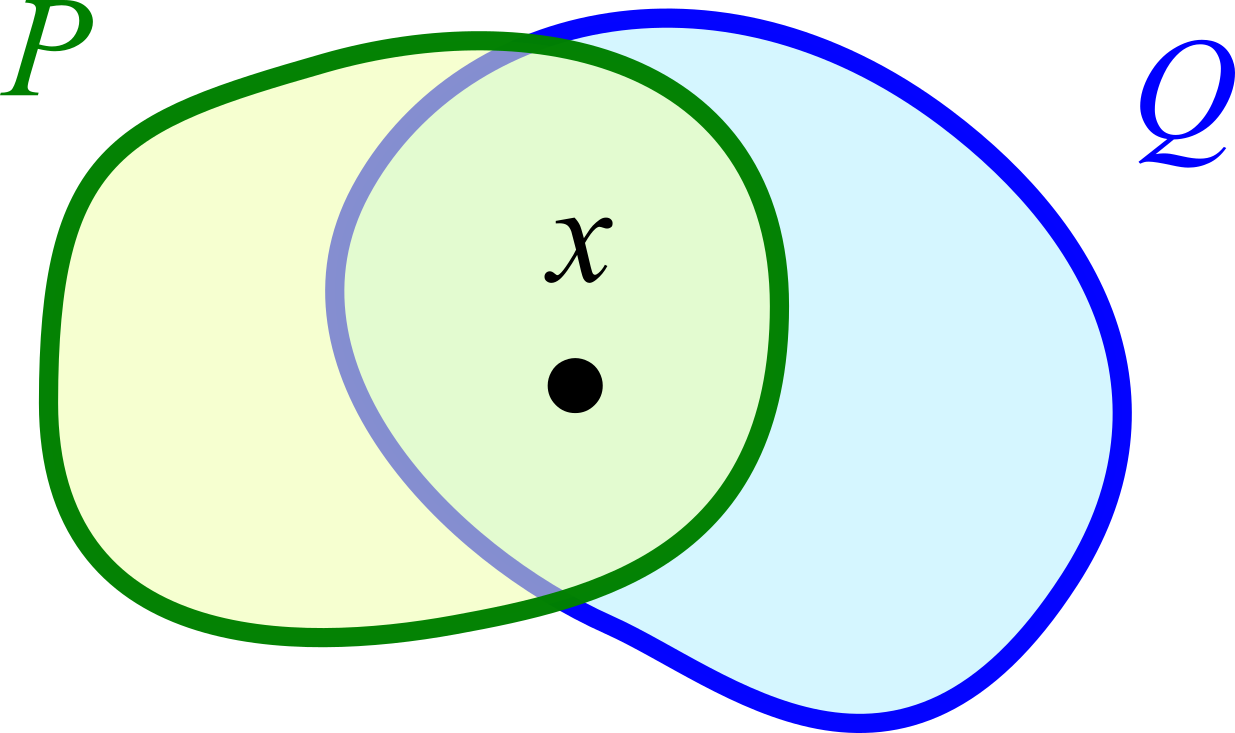
\includegraphics[scale=0.7]{Venn-diagram.png}}}
\end{equation}
The motivation for introducing geometric models:  Since we need to perform search among logic formulas, \uline{it may be desirable to represent formulas such that they can continuously ``morph'' into each other}:
\begin{equation}
\vcenter{\hbox{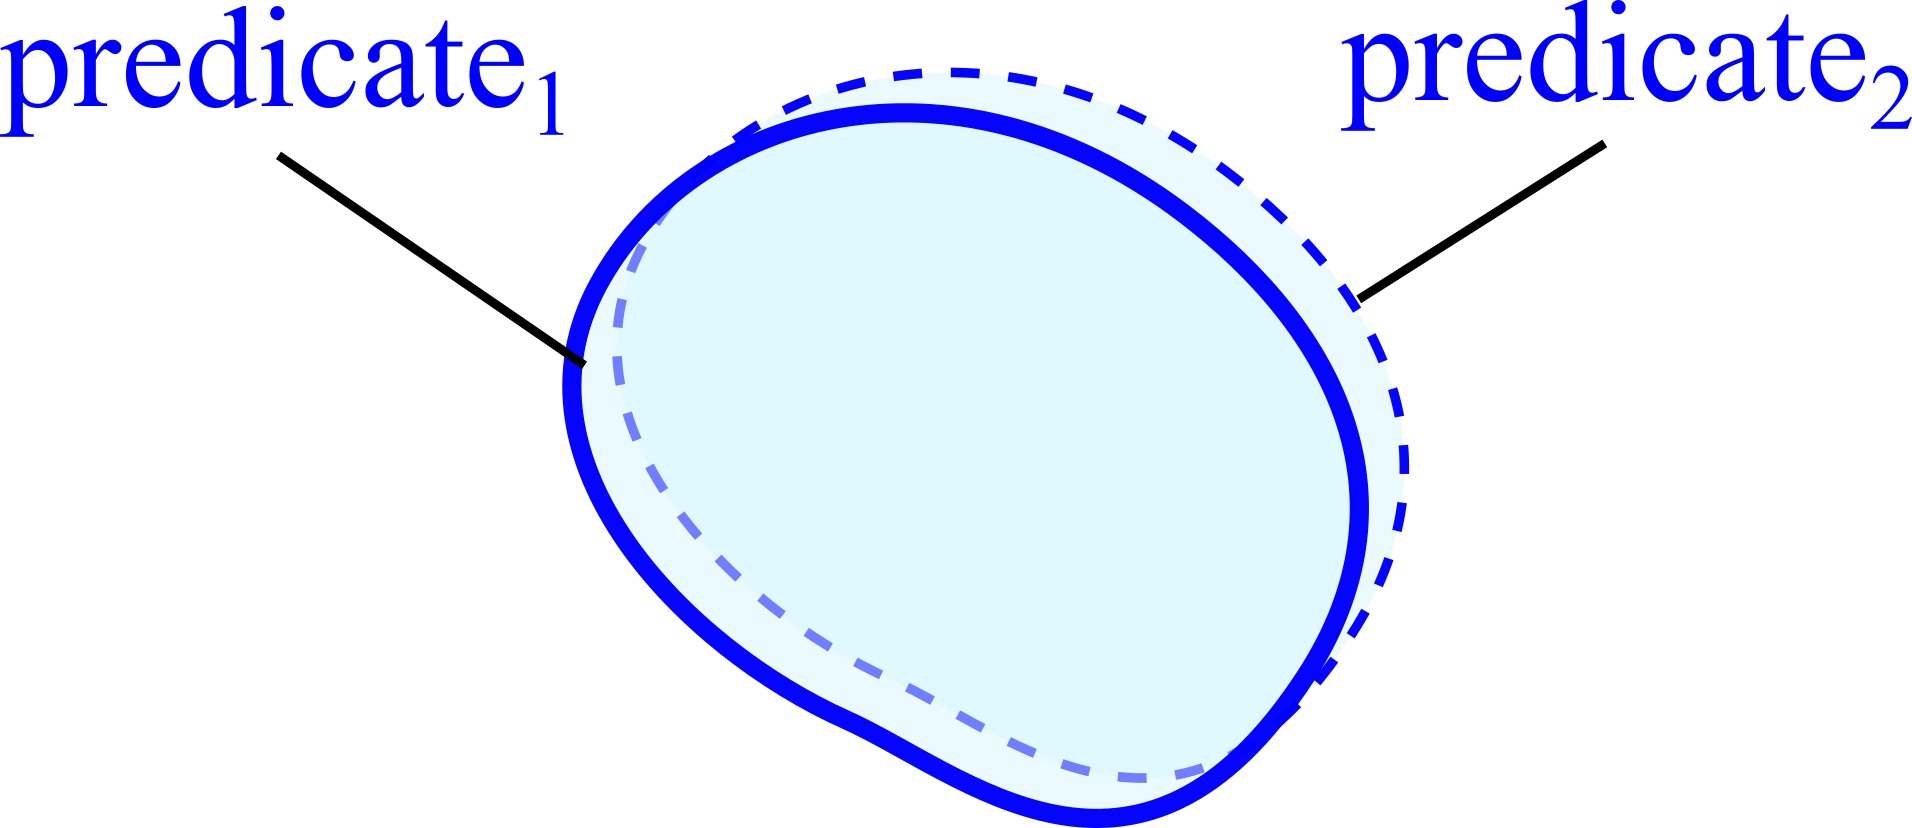
\includegraphics[scale=0.7]{nearby-predicates.png}}}
\end{equation}

%\cc{这些 geometric ``\textbf{regions}'' 很容易用神经网络做到。 如果 $\vec{F} =$ 神经网络,则:
%}{
%These geometric ``\textbf{regions}'' are easy to implement with neural networks.  If $\vec{F} =$ a neural network, then:}
%\begin{equation}
%\vec{F}(\vec{x}) = 0
%\end{equation}
%\cc{定义了一个 hyper-surface of co-dimension 1,它将周围的空间分割为 $> 0$ 和 $< 0$ 两部份。 
%}{
%defines a hyper-surface of co-dimension 1, which divides the ambient space into 2 parts: $> 0$ and $< 0$.}

In classical logic this is not possible.  For example, $\mbox{Love}(x,y)$ and $\mbox{Like}(x,y)$ may be similar in meaning, but the transition from one to the other requires a discrete ``jump''.

We propose to use \textbf{points} to represent first-order objects (\textit{eg} ``John'') and \textbf{regions} (\textit{ie}, point sets, open sets) to represent predicates and relations (\textit{eg} ``Love'').  It is possible to use a \textit{dual} model in which points and regions are swapped.

A caveat is that the points and regions must be \textit{labelled} entities.  For example, it is not sufficient to know that the point (John, Mary) belongs to a relation, but it matters whether that relation is Love or Hate.  In other words, the \textit{identity} of the region matters.

\footnotesize
$\NewSym{../UnderConst.png}$ \quad \parbox{0.9\textwidth}{
Previously I made the mistake of forgetting the labels associated with geometric regions, thus falsely simplifying the algorithm and claimed success.  It turns out that the presence of labels forces us to handle the rewriting function on the \textbf{syntactic} level, and the geometric shapes of models do not seem to make an essential difference (to my disappointment).  So this idea needs re-consideration.  }
\normalsize

% 根据 范畴论 的看法,一个集合里的\textbf{元素},是一个 $\mathbf{1} \rightarrow \mathbf{Set}$ 的 mapping。  如果我们不想要「一粒粒」的元素,或许可以用 $\mathbb{R} \rightarrow \mathbf{Set}$ 这样的 mapping? 

\cc{总括来说,这个方案是:
}{
This representation scheme can be summarized as follows:}
\begin{eqnarray}
\mbox{model } \mathscr{M} &=& \mbox{geometric model of set theory} \nonumber \\
\mbox{rewriter} &=& \mbox{functor } \mathscr{M} \rightarrow \mathscr{M}
\end{eqnarray}
\cc{但我们需要一个 \uline{可以连续变化的} model of set theory,或许可以用某种 fuzzy topology 来达成?  例如:
}{
But we need a \uline{model of set theory that can be continuously changed}, maybe it can be achieved with some kind of fuzzy topology? E.g:}
\begin{equation}
\vcenter{\hbox{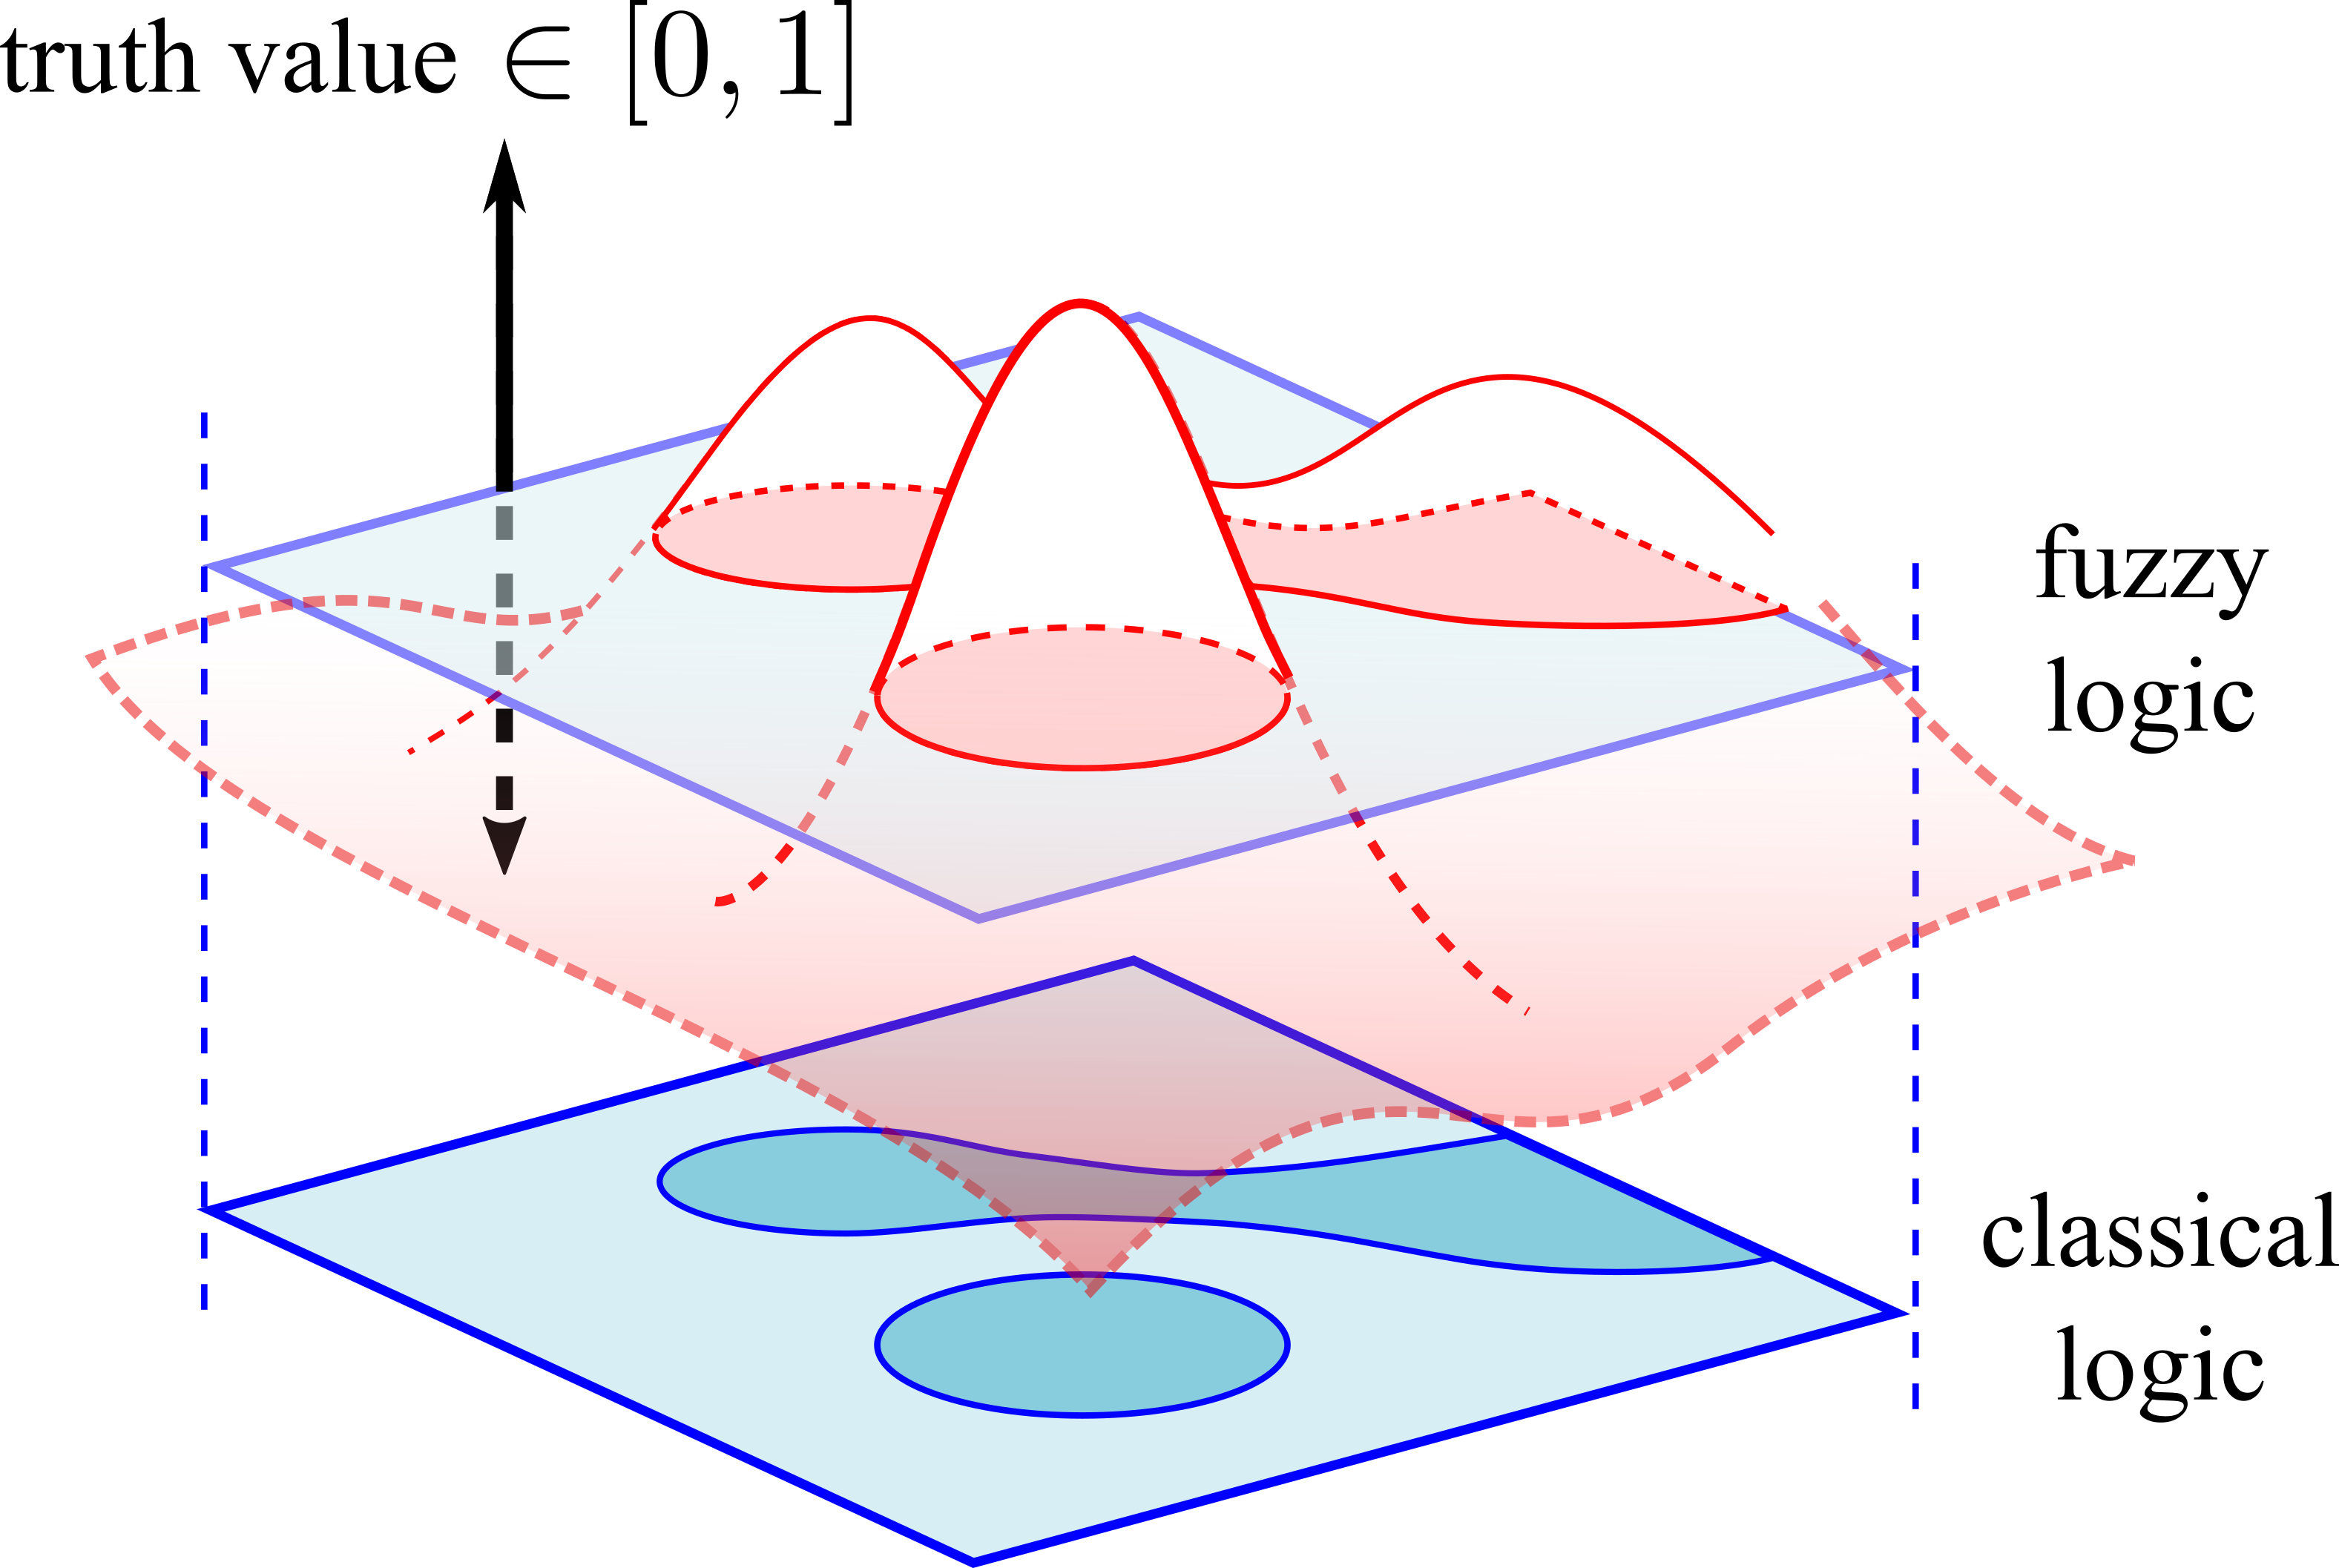
\includegraphics[scale=0.6]{fuzzy-geometric-model.png}}}
\end{equation}
% 和传统 fuzzy logic 不同,我将 ``neutrality'' $\frac{1}{2}$ 移到 0 的位置,这样更符合直观。 
\cc{其需要定义的 boundary of regions 维数 高了 1 度。
}{
The boundary of regions that need to be defined is 1 degree higher.}

\footnotesize
\cc{但这里有个问题: 逻辑上,两个式子之间的 semantic distance 可以定义为由一个式子推导到另一个式子所需的 proof steps 个数(它还取决於 $\KB$ 内的其他式子),但根据 Turing 在 1936 年证明的的 halting problem 定理,这个 distance 是\textbf{不可计算的}。\footnote{The logic semantic distance is similar to \textbf{Kolmogorov complexity} but not exactly the same.  Kolmogorov complexity is incomputable but can be approximated \parencite{Li2008}.}  换句话说,在逻辑式子的空间上不可能有完全确定的 semantic metric。  我们的 $\vec{u} = \Theta$ 类似於逻辑式子,如果在 $\Theta$ 上能定义 gradient $\nabla_\Theta$,似乎有矛盾。 会不会 \textbf{fuzzy topology} 能做到 semantic metric 的近似?  这取决於 fuzzy geometric model 的 rewriting function space $\Theta$ 是不是 \textbf{metrizable} (\textit{cf} \parencite{Goubault-Larrecq2013}).  在未来我会更详细研究这点。
}{
But here's the problem: Logically, the semantic distance between two expressions can be defined as the number of proof steps required to derive from one formula to another (it also depends on the contents of $\KB$), but according to the halting theorem that Turing proved in 1936, this distance is \textbf{incomputable}. \footnote{The logic semantic distance is similar to \textbf{Kolmogorov complexity} but not exactly the same. Kolmogorov complexity is incomputable but can be approximated \parencite{Li2008}.}  In other words, it is impossible in the space of logic formulas to have an exactly defined semantic metric.  Our $\vec{u} = \Theta$ is analogous to logic formulas;  If we can define a gradient $\nabla_\Theta$ on $\Theta$, it seems to lead to contradiction.  Can \textbf{fuzzy topology} be able to approximate the semantic metric?  This depends on whether the fuzzy model-rewriting function space $\Theta$ is \textbf{metrizable} or not (\textit{cf} \parencite{Goubault-Larrecq2013}).  Further investigation is needed.}
\normalsize
\begin{equation}
\vcenter{\hbox{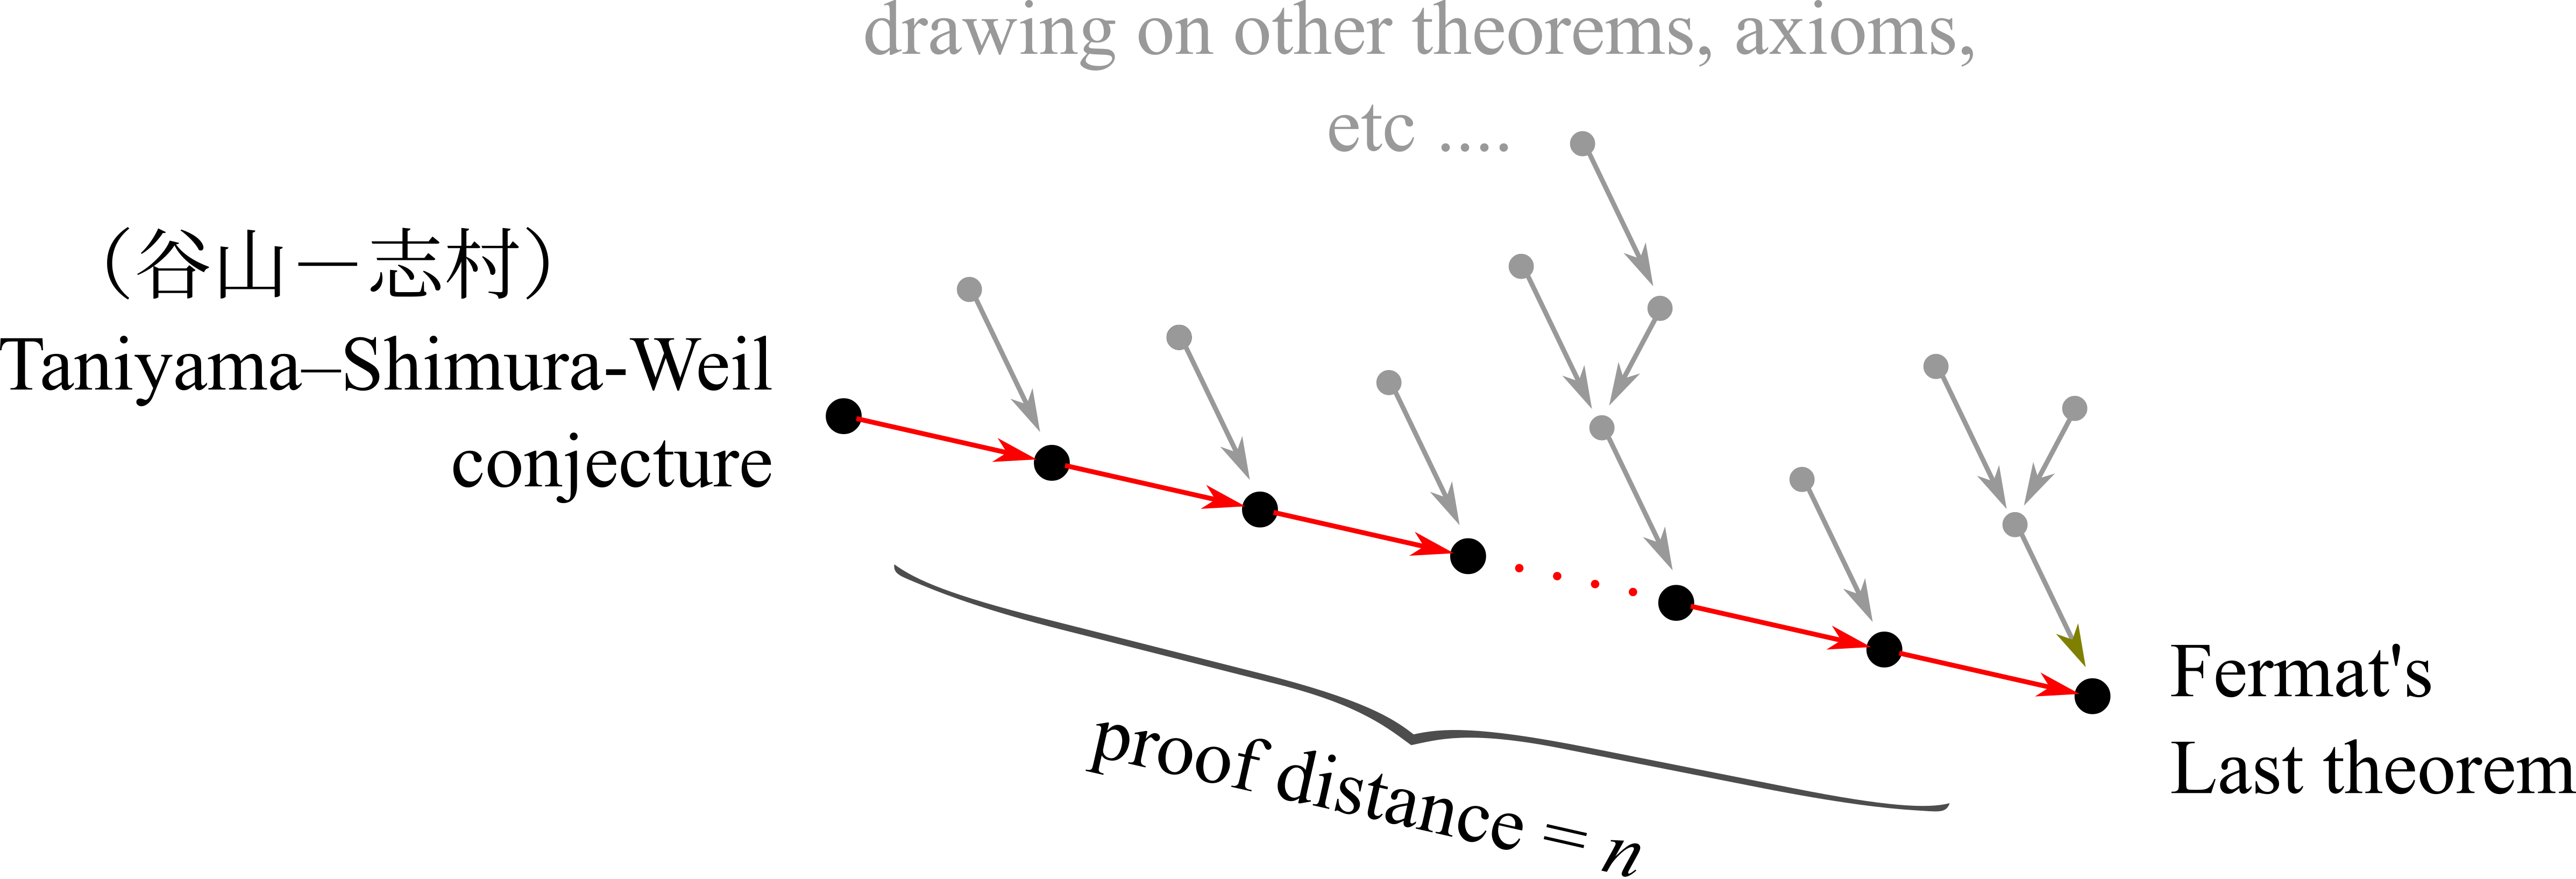
\includegraphics[scale=0.6]{proof-distance.png}}}
\end{equation}

\textbf{The ``plateau problem'':}  From \parencite{Bergadano1996}:  Researchers have discovered that, during the inductive learning of logic formulas, it may happen that in the body of the correct clause, the gain remains low and constant (on a plateau) until one final important literal concludes the computation and brings the gain to a local maximum.  An example is the following target clause:
\begin{equation}
\parbox{0.7\textwidth}{
\code{append(X,Y,Z)  :-  list(X), head(X,X1), tail(X,X2),  \\
\quad \quad	append(X2,Y,W), cons(X1,W,Z).}}
\end{equation}

% 如果想用传统的 基於 differentials 的 optimization 技巧,似乎最低要求是 domain 上的 topology、continuity 和 compactness,然后才可以定义例如 Fr\'{e}chet derivative. \parencite{Henrot2018}

% 当然,如果改写的能力太弱,则会 ``throw the baby out with the water'',亦即丧失了一阶逻辑的\textbf{泛化}能力。  同时,要从 optimization 的角度考虑,什么形式的改写才最有利於速度。  模型的 representation 也是一个考虑因素: 它应该有某种良好的 \textbf{metric},这 metric 近似 semantic distance,而不是纯粹基於 logic syntax。 事实上,完美的 semantic metric 是\textbf{不可计算的},因它是 Kolmogorov complexity.

\begin{center}
\rule{0.4\textwidth}{.6pt}
\end{center}

\cc{以下主要分析 plan A 和 B(它们已经是可行的)。 Plan A 直接用 discrete optimization,所以不需要 metric space。  Plan B 用神经网络,它的 weights $\in \mathbb{R}$ 是连续空间,但这神经网络是作用在 graph 上,后者仍然是离散结构。
}{
The following main analysis of plan A and B (they are already feasible). Plan A uses discrete optimization directly, so no metric space is required. Plan B uses a neural network whose weights $\in \mathbb{R}$ is a contiguous space, but this neural network acts on the graph, which is still a discrete structure.}

\section{Plan A: genetic algorithm}
\label{COCO}

\begin{tcolorbox}[ams equation, colback=yellow, colframe=white]
\cc{
\mbox{放弃梯度下降}}{
\mbox{\textbf{abandon} gradient descent}
}
\end{tcolorbox}
\begin{eqnarray}
\cc{
\mbox{model } \mathscr{M} &=& \mbox{符号逻辑式子} \nonumber \\
}{
\mbox{model } \mathscr{M} &=& \mbox{symbolic logic formula} \nonumber \\
}
\cc{
\mbox{rewriter} &=& \mbox{符号逻辑式子 + 经典 AI 逻辑引擎}}{
\mbox{rewriter} &=& \mbox{symbolic logic formula + classical AI logic engine}
}
\end{eqnarray}

\cc{GA 本来就非常适合\textbf{离散}的搜寻空间,它和逻辑结构很兼容,在这条路线上已经没有理论上的 obstructions. 
}{
GA is very suitable for the \textbf{discrete} search space. It is compatible with the logical structure. There is no theoretical obstructions on this route.}

% \section{Plan A: 协同进化 (COCO)}

% Substitution 的麻烦令我想到 \uline{放弃用 neural network 直接处理逻辑,而是用 hybrid 的 神经/逻辑 混合}: 视觉神经用 deep neural network,到高层次转用符号逻辑表述,后者用 genetic algorithm 做学习。

\cc{首先需要一个 logic-based \textbf{rule engine},它负责 forward-chaining(正向逻辑推导),这完全是经典 AI 的范围。 例如 经典的 Soar architecture [Carnegie-Mellon 大学] 就是一个 rule-base 引擎。 % 还有我这一代的 OpenCog, OpenNARS, 和我写的 Genifer\footnote{Genifer 仍未到达 production stage.},或许还有更新一代的 AGI 系统(?)  
}{
First you need a logic-based \textbf{rule engine}, which is responsible for forward-chaining, which is completely the scope of classic AI. For example, the classic Soar architecture [Carnegie-Mellon University] is a rule-base engine.}
% and my generation of OpenCog, OpenNARS, and my Genifer\footnote{Genifer have not yet reached the production stage.}, and perhaps a newer generation of AGI systems (?)}

% 经典逻辑 AI 的樽颈问题是 \uline{rules 的学习算法太慢},
%\begin{itemize}
%\item plan A: 继续用经典逻辑引擎,用 genetic algorithm 做学习算法
%\item plan B: 将逻辑记忆映射到向量空间,再用神经网络学习逻辑 rules
%\end{itemize}

\cc{基因算法的 population 是由个别的逻辑 rules 组成,但 winner 并不是单一条 rule,而是一整套 rules(最高分的 $N$ 个)。 这叫 \textbf{cooperative co-evolution}(COCO)。  
}{
The genetic algorithm's population is composed of individual logical rules, but the winner is not a single rule, but a set of rules (the highest score of $N$). This is called \textbf{cooperative co-evolution}(COCO).}

\cc{输入和输出是 logic formulas,其实更易处理。 
}{
Inputs and outputs are logic formulas, which are actually easier to handle.}

\cc{整个系统仍然是基於 reinforcement learning 的,但不需要直接做 RL,因为那些 rules 其实就是 \textbf{actions},每条 rule  的 probabilistic strength 就像 $Q$-learning 中 $Q$值的作用。 
}{
The whole system is still based on reinforcement learning, but you don't need to do RL directly, because those rules are actually \textbf{actions}, and the probabilistic strength of each rule is like the $Q$ value in $Q$-learning.}

\cc{[ 我还未有时间 survey COCO 的实践理论。 ]
}{
[I have not had time to explore the practical theory of COCO. ]}

\section{Plan B: neural network / deep learning}

\cc{馀下大部份篇幅都是为了解决如何用 NN 实现 经典逻辑引擎 的问题,特别是 variable substitution 的问题,最后发觉问题的癥结在於缺少了 short-term memory 的机制。
}{
Most of the time is to solve the problem of how to implement the classic logic engine with NN, especially the problem of variable substitution. Finally, the crux of the problem is the lack of short-term memory mechanism.}

\cc{解决办法是 用 graph 做\textbf{记忆系统},用神经网络做 graph re-writing,亦即 Google / DeepMind 提出的 graph neural network,这是一种 ``hybrid'' architecture.
}{
The solution is to use graph as \textbf{memory system} and use neural network for graph re-writing, which is the graph neural network proposed by Google / DeepMind. This is a ``hybrid'' architecture.}

\subsection{\cc{神经网络 处理 substitutions 的困难}{NNs have difficulty handling substitutions}}
\label{NN}

\cc{考虑上节讲过的 逻辑 rule(``失恋则不开心''):
}{
Consider the logic rule that was mentioned in the previous section (``Love is not happy''):}
\begin{equation}
\forall x,y. \; x \heartsuit y \wedge \neg y \heartsuit x \rightarrow \frownie{} x
\end{equation}
\cc{这个 rule 的 \textbf{前件} (antecedent) 要成立,必须 \uline{两次出现的 $a$ }\textbf{\uline{相等}}\uline{、两次出现的 $b$ }\textbf{\uline{相等}}:
}{
The \textbf{predecessor} (antecedent) of this rule must be established, and must be \uline{$a$ }\textbf{\uline{equal}}\uline{, twice appearing, $b$ }\textbf {\uline{equal}}:}
\begin{equation}
\vcenter{\hbox{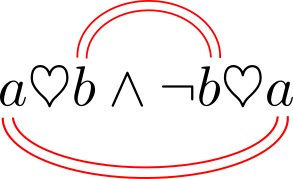
\includegraphics[scale=0.6]{antecedents-equal.png}}}
\end{equation}
\cc{而且,要产生正确的 \textbf{后件} (consequent),需要从前件中将 $a$ \textbf{copy} 过来:
}{
Also, to produce the correct \textbf{postsent} (consequent), you need to pass $a$ \textbf{copy} from the previous:}
\begin{equation}
\vcenter{\hbox{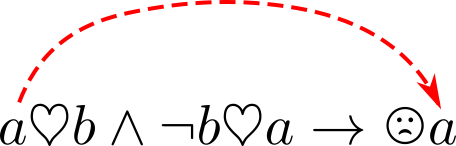
\includegraphics[scale=0.6]{consequent-copy.png}}}
\end{equation}
\cc{\uline{这两个动作(\textbf{compare} 和 \textbf{copy})都是用神经网络 很难做到的}。  但它们是 variable substitution 的本质,也是 谓词逻辑 麻烦之处。 换句话说,很难用一个 monolithic 的 end-to-end 神经网络 一口气完成这两个动作:
}{
\uline{These two actions (\textbf{compare} and \textbf{copy}) are hard to do with neural networks}. But they are the essence of variable substitution and the trouble of predicate logic. In other words, it is difficult to accomplish these two actions in one breath with a monolithic end-to-end neural network:}
\begin{equation}
\vcenter{\hbox{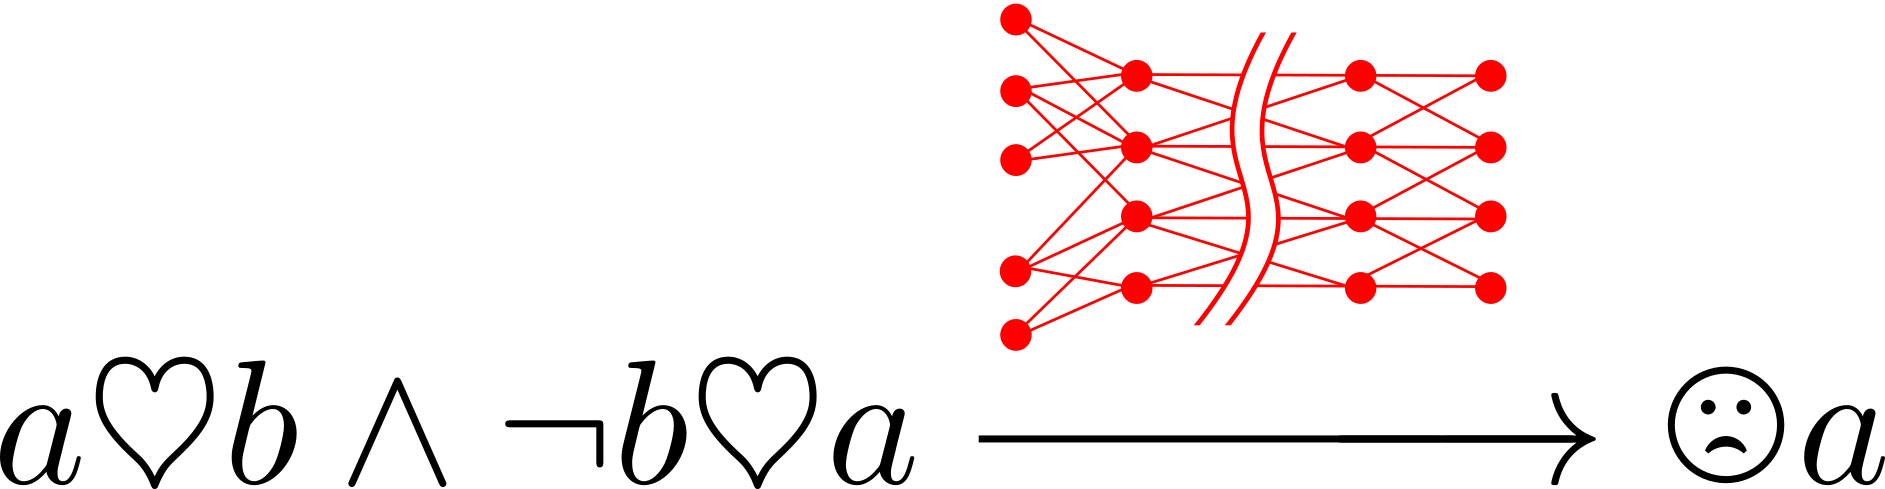
\includegraphics[scale=0.6]{monolithic-NN.png}}}
\end{equation}

\cc{首先考虑\textbf{后件}的 copy 问题。 为简单起见,假设逻辑 variable $z$ 对应於 输入向量 $\vec{x}$ 中的某些分量,例如 $x_i$.  Copy 的作用是将 $x_i$ 抄到 $y_j$ 的位置:
}{
First consider the copy problem of \textbf{poster}. For simplicity, assume that the logical variable $z$ corresponds to some component of the input vector $\vec{x}$, such as $x_i$. The purpose of Copy is to copy $x_i$ to the $y_j$ position:}
\vspace*{10pt}
\begin{equation}
\vec{F}: \; (x_1, ..., {\color{red} x_i} \tikzmark{a}, ... , x_n) \mapsto (y_1, ... , \tikzmark{b} {\color{red} y_j} , ... , y_n)
\begin{tikzpicture}[overlay,remember picture,out=45,in=135,distance=1.1cm]
  \draw[->,red,shorten >=7pt,shorten <=7pt] (a.center) to node [auto, above=2pt] {$id$} (b.center);
\end{tikzpicture}
\end{equation}
\cc{这要求神经网络的函数曲面穿过某些 diagonal 线,如下图:
}{
This requires the function surface of the neural network to pass through some diagonal lines, as shown below:}
\begin{equation}
\vcenter{\hbox{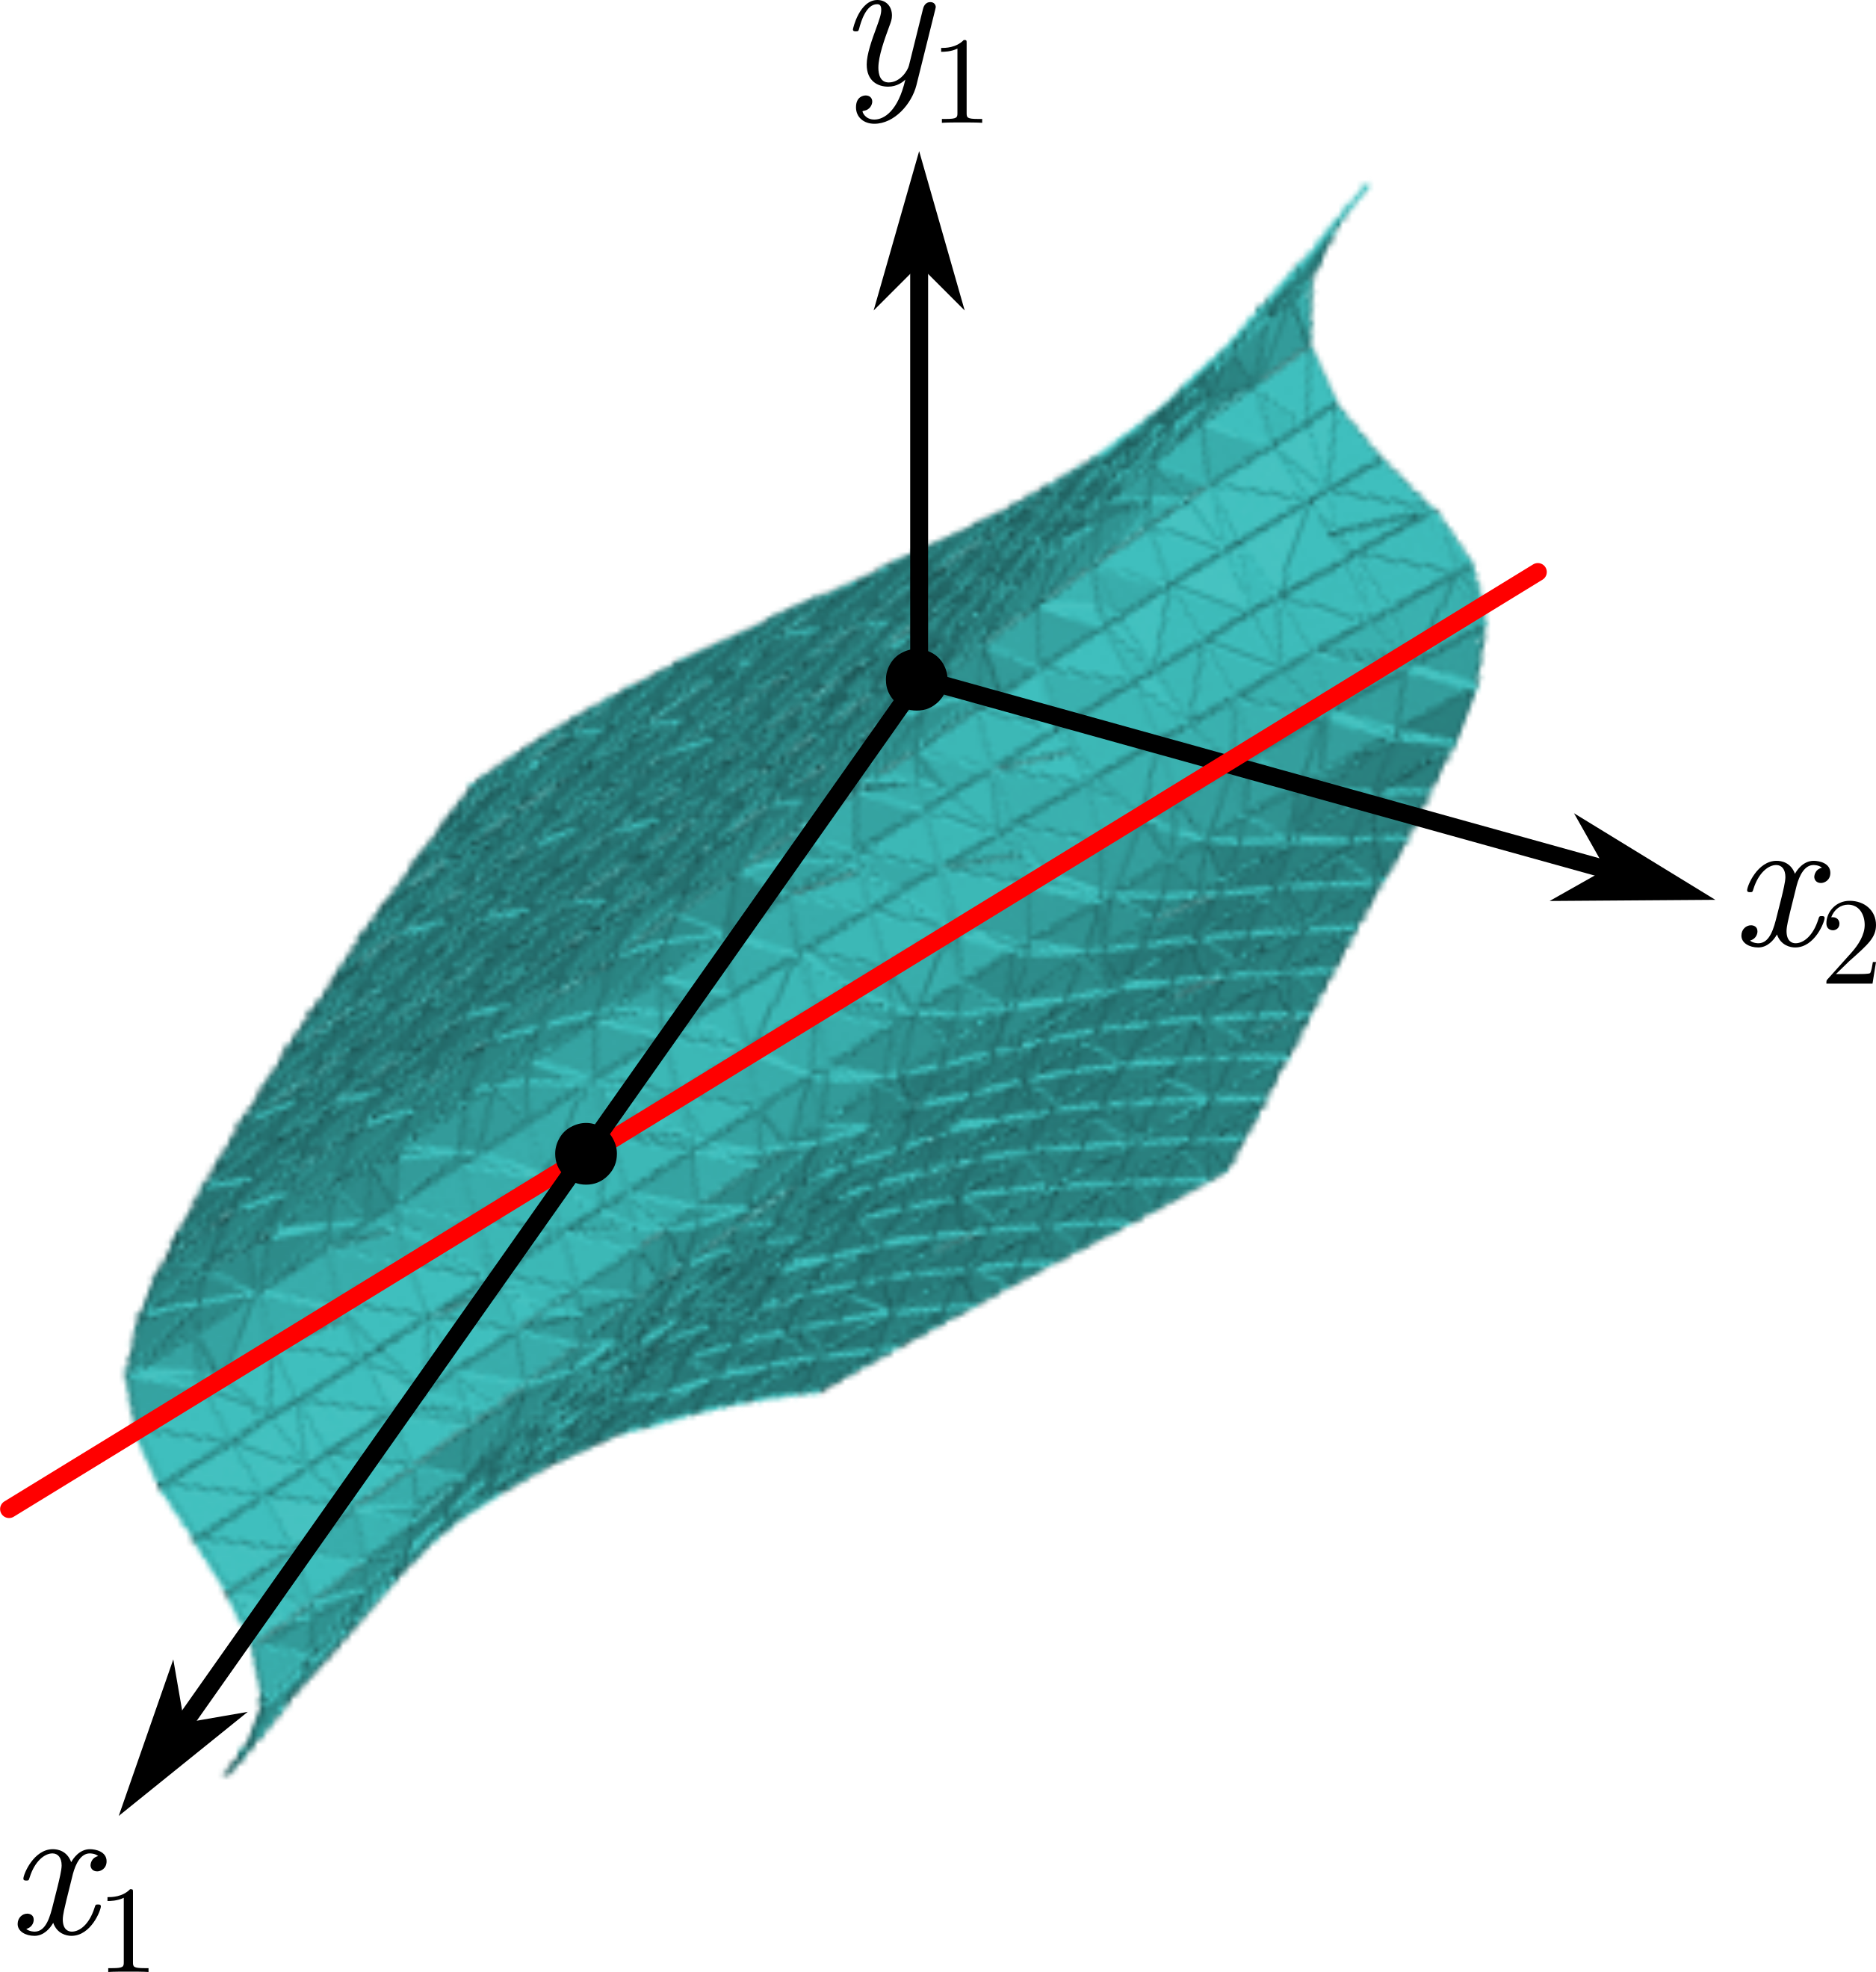
\includegraphics[scale=0.4]{diagonal.png}}}
\end{equation}
\cc{以下是一个简单的 copier 神经网络(所有权重 = 1,其他权重 = 0 没有显示):
}{
The following is a simple copier neural network (ownership weight = 1, other weights = 0 not shown):}
\begin{equation}
\vcenter{\hbox{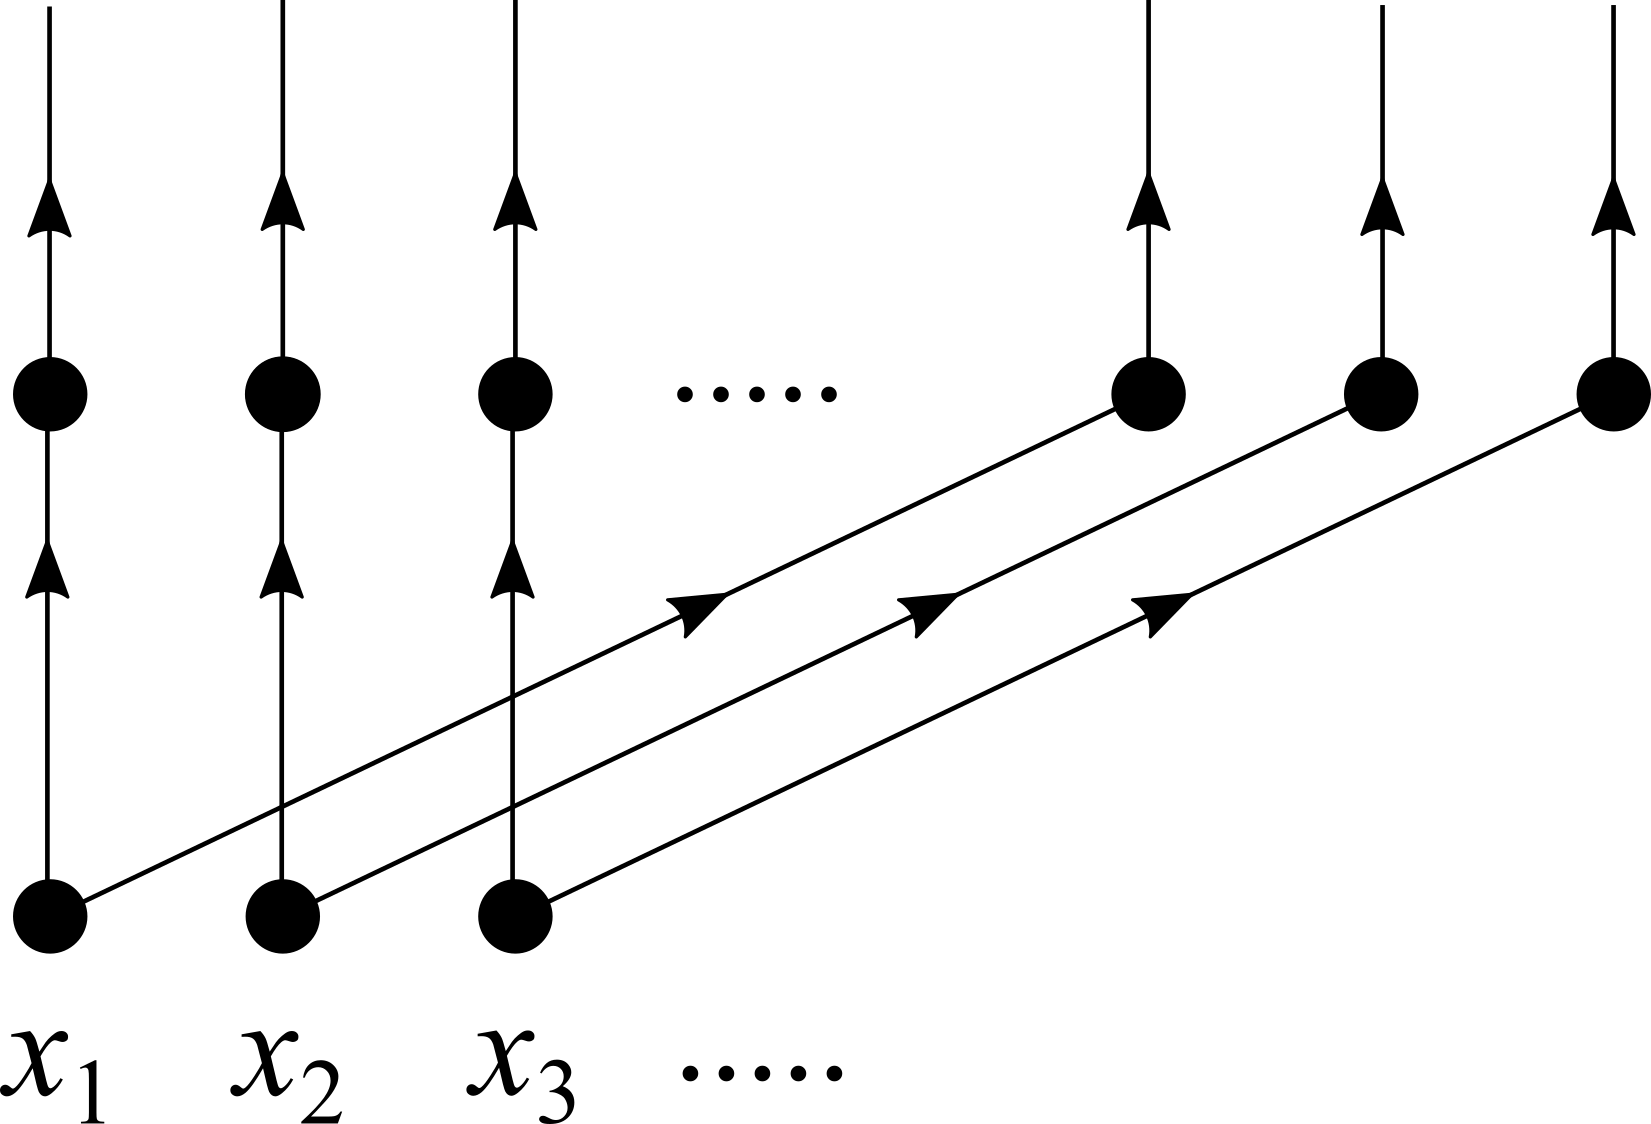
\includegraphics[scale=0.7]{NN-copying.png}}}
\end{equation}
\cc{一个输入 dim = $n$,输出 dim = $2 n$ 的神经网络,fully connected 的话需要训练 $2 n^2$ 个 weights。 但我还未有时间试验一般多层神经网络学习这个动作需要训练多久。 
}{
A neural network with input dim = $n$ and output dim = $2 n$, if fully connected, needs to train $2 n^2$ weights. But I haven't had time to test how long it takes to train a multi-layer neural network to learn this action.}

\cc{其次,考虑\textbf{前件}的成立,一种可行的\textbf{几何图像}是这样的 \footnote{这只是众多可能的 representations 之一,但似乎任何「几何」形式的 representations 都有类似问题。 除非我们考虑有 ``procedural'' 特点的 representations? 以下会讨论.... }:
}{
Second, consider the establishment of \textbf{frontware}, a viable \textbf{geometric image} is such a \footnote{this is just one of many possible representations, but it seems that any "geometric" form of representations has similar problems. . Unless we consider representations with the characteristics of ``procedural''? The following will discuss .... }:}
\begin{equation}
\vcenter{\hbox{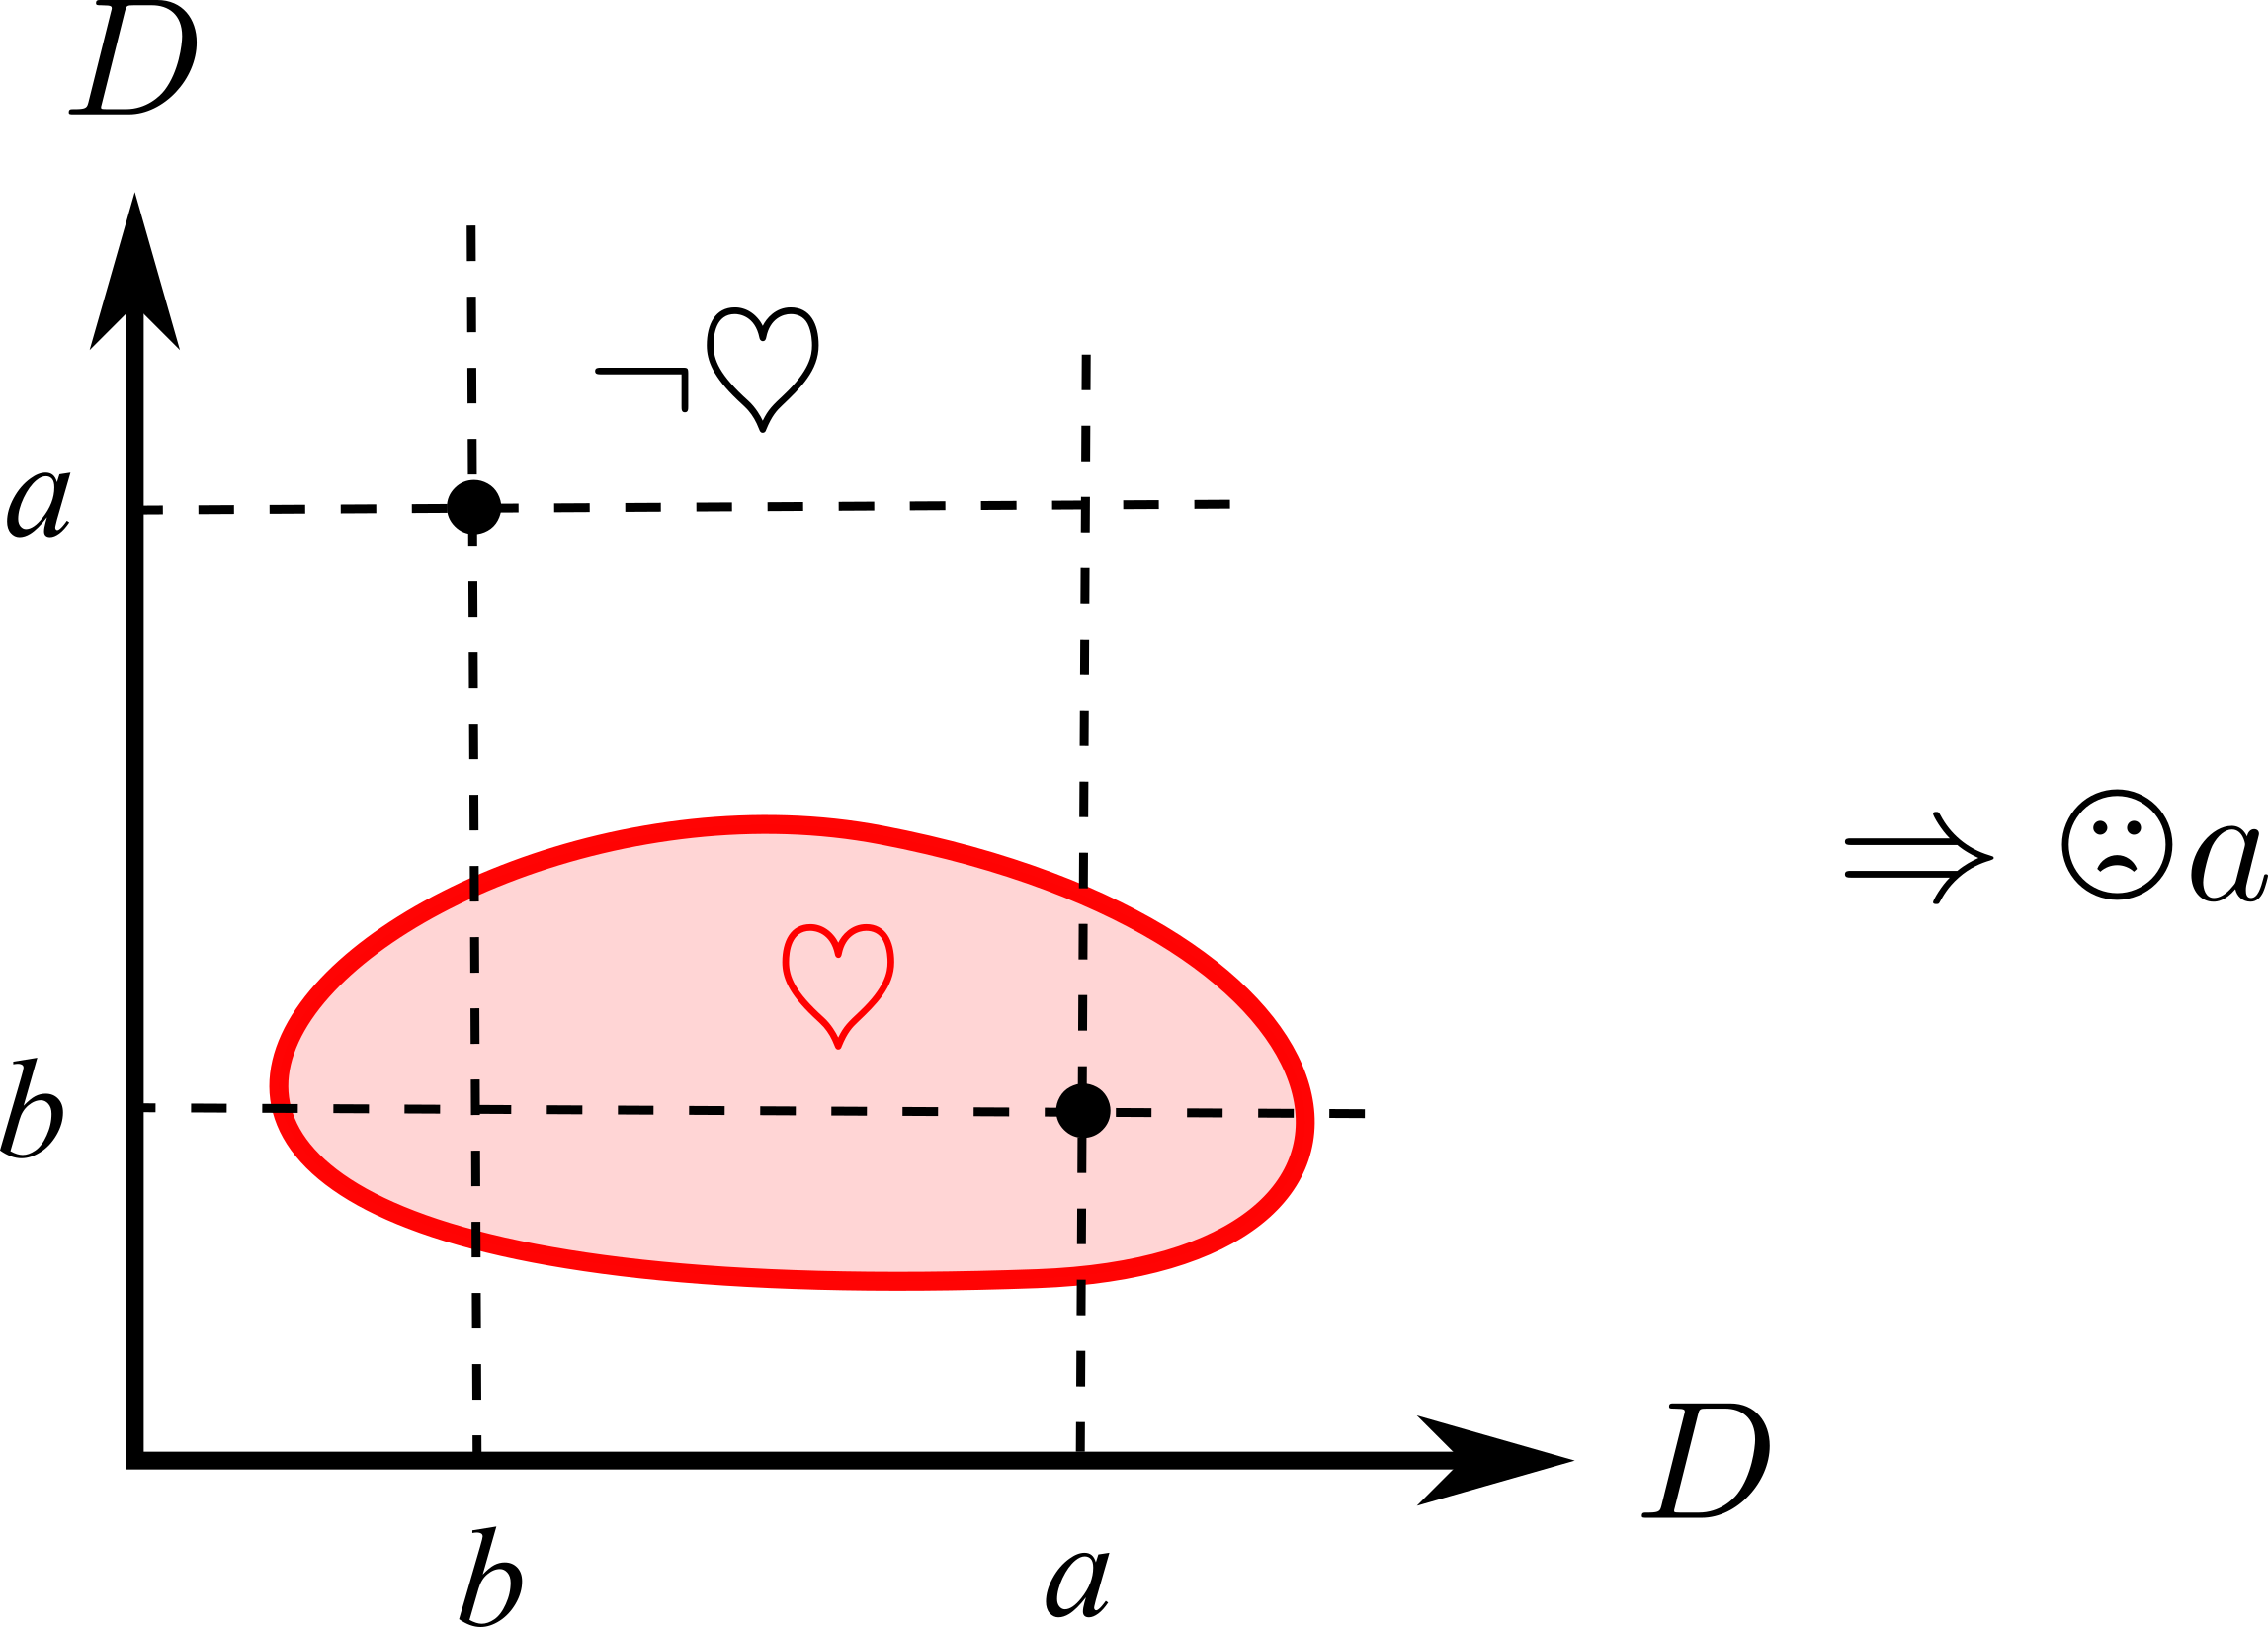
\includegraphics[scale=0.6]{heart-break.png}}}
\end{equation}
\cc{$\in$ 很容易用神经网络解决,例如可以定义 $\heartsuit$ 为一个神经网络:
}{
$\in$ is easy to solve with a neural network, for example $\heartsuit$ can be defined as a neural network:}
\begin{equation}
\heartsuit (\vec{x}) = \begin{cases}
0 & \vec{x} \notin \mbox{region}\\
1 & \vec{x} \in \mbox{region}
\end{cases}
\end{equation}
\cc{但即使这样,仍然馀下一个 pattern matching (comparison) 问题:
}{
But even then, there is still a pattern matching (comparison) problem:}
\begin{eqnarray}
\vec{p}_1 = (\tikzmark{a1} \vec{a}, \vec{b} \tikzmark{b1}) &\in& \heartsuit \nonumber \\
&& \nonumber \\
\vec{p}_2 = (\tikzmark{b2} \vec{b}, \vec{a} \tikzmark{a2}) &\in& \neg \heartsuit
\begin{tikzpicture}[overlay,remember picture]
  \draw[-, red, shorten <=20pt, transform canvas={shift={(-3pt,13pt)}}] (a1.center) to (a2.center);
  \draw[-, red, shorten <=20pt, transform canvas={shift={(-6pt,13pt)}}] (a1.center) to (a2.center);
  \draw[-, red, shorten <=20pt, transform canvas={shift={(5pt,13pt)}}] (b1.center) to (b2.center);
  \draw[-, red, shorten <=20pt, transform canvas={shift={(2pt,13pt)}}] (b1.center) to (b2.center);
\end{tikzpicture}
\end{eqnarray}
\cc{以下是一个简单的用 RNN 神经网络 模拟的 comparator(所有 = 0 的权重 没有显示):
}{
The following is a simple comparator simulated with the RNN neural network (all = 0 weights are not shown):}
\begin{equation}
\vcenter{\hbox{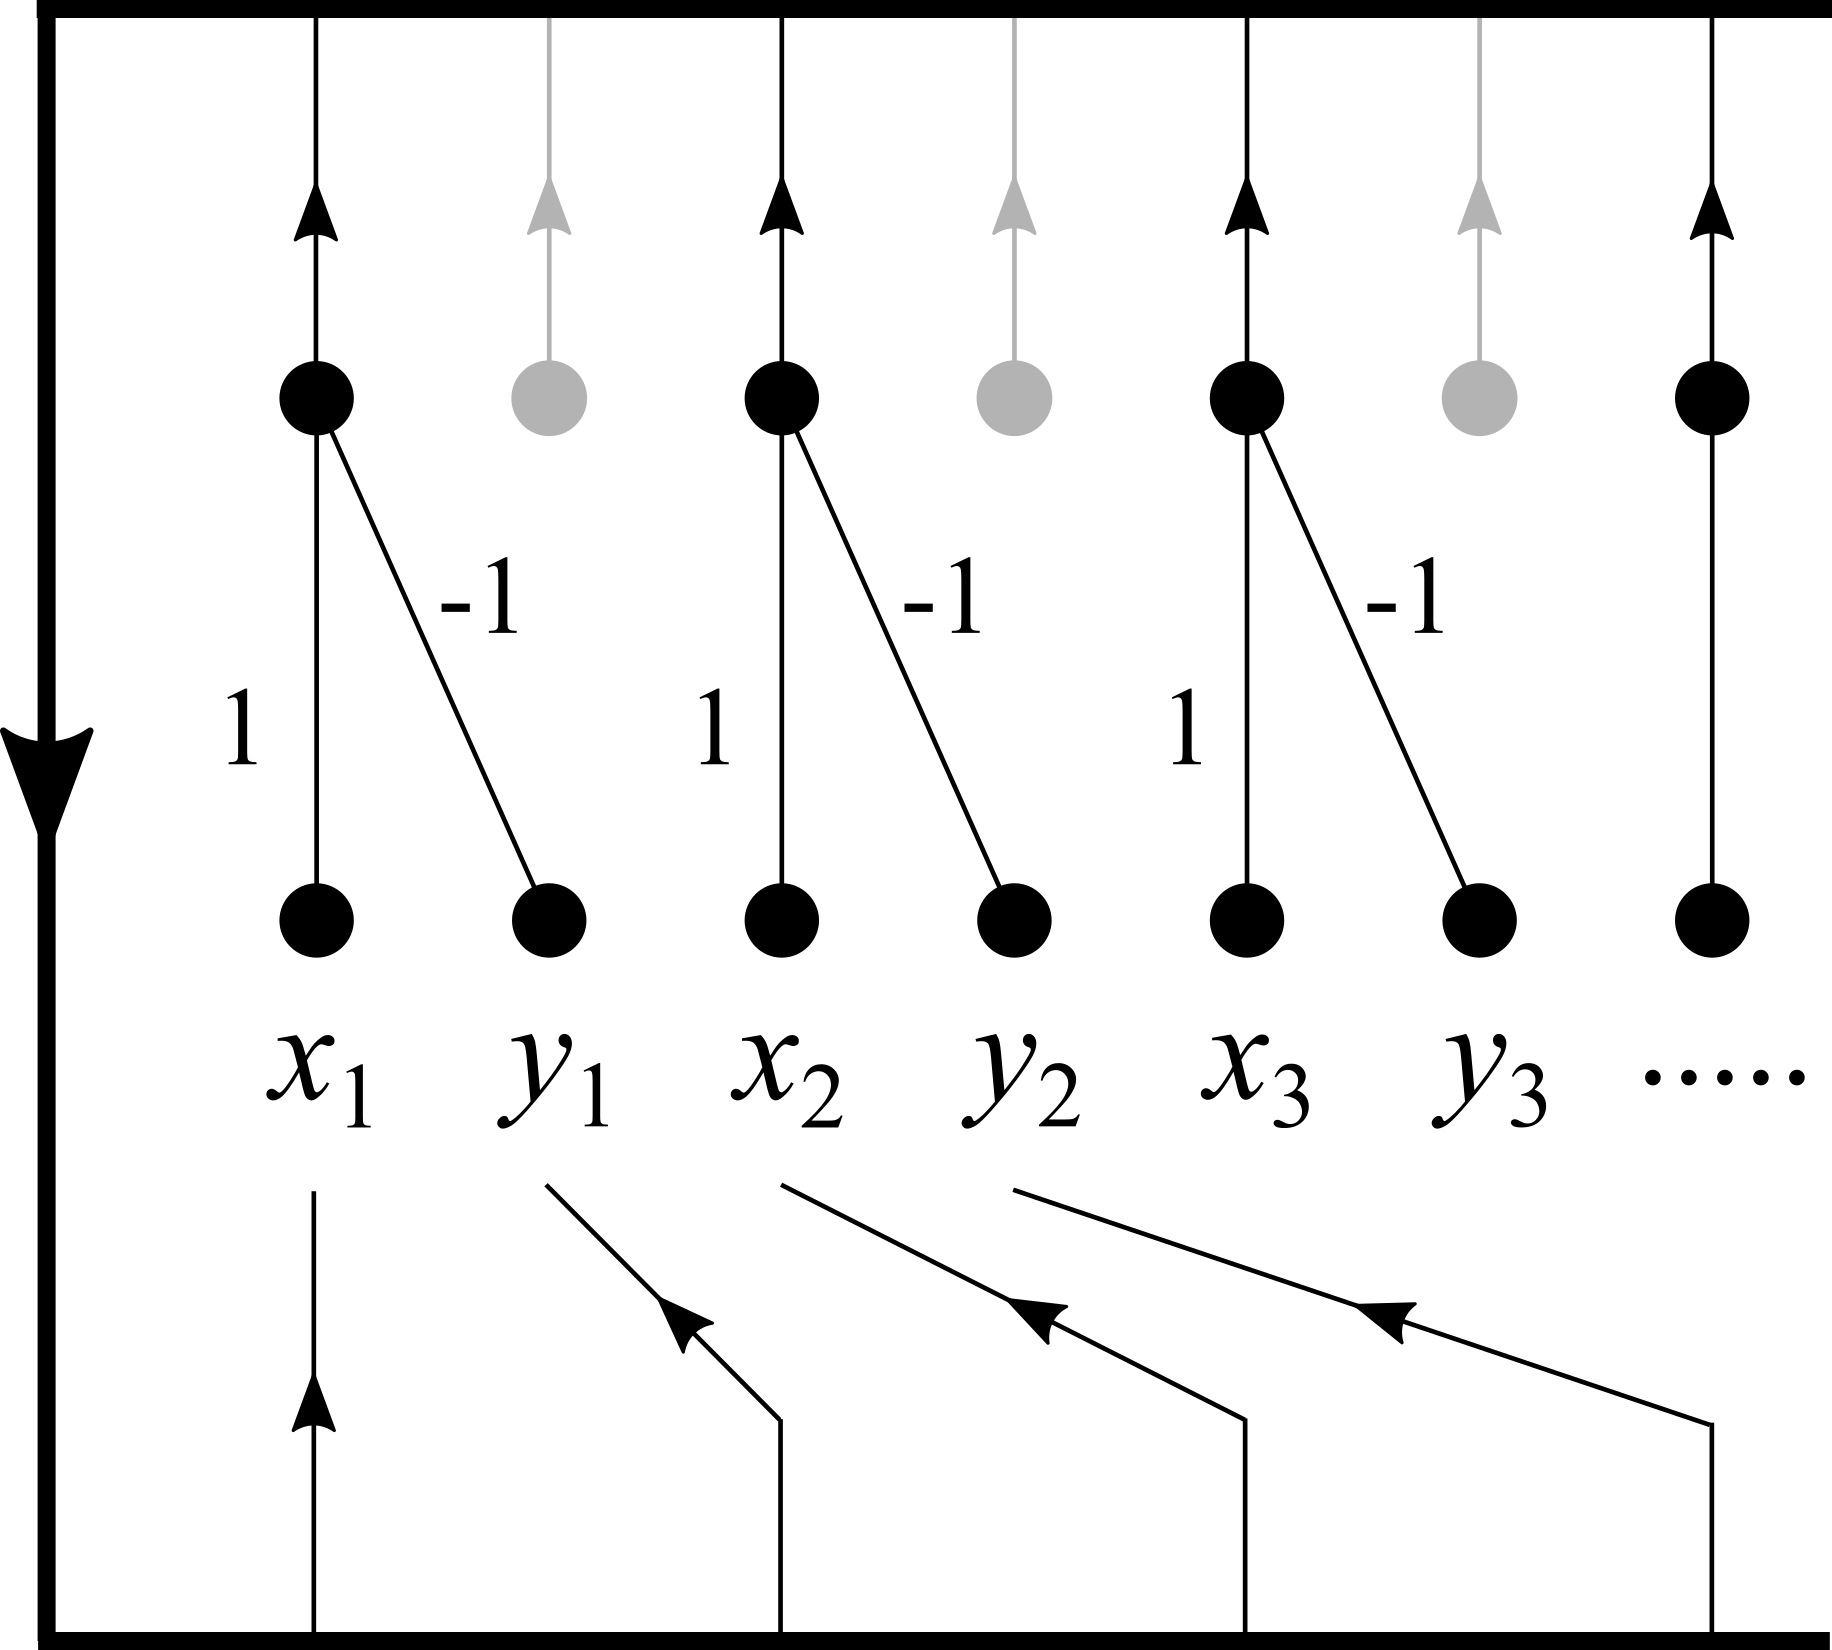
\includegraphics[scale=0.7]{NN-comparator.png}}}
\end{equation}
\cc{在 iterate $n$ 次之后,最左边的输出 会是 $\vec{x} \stackrel{?}{=} \vec{y}$ 的真假值。 假设 输入维数是 $2 n$,需要训练 $(2 n)^2$ 个 weights。
}{
After iterate $n$ times, the leftmost output will be the true or false value of $\vec{x} \stackrel{?}{=} \vec{y}$. Assuming the input dimension is $2 n$, you need to train $(2 n)^2$ weights.}

\cc{结论: 根据以上分析,用 NN 模拟 copier 和 comparator 似乎不算很难,但实际上还要将这些「元件」配合 short-term memory 使用,整个 architecture 仍然是未知的。
}{
Conclusion: Based on the above analysis, it seems not very difficult to simulate copier and comparator with NN, but in fact, these "components" are used in conjunction with short-term memory, and the entire architecture is still unknown.}

\subsection{\cc{「分布式」知识表述}{``Distributive'' representations}}

% Distributive representation 是针对神经网络而言的,因为神经网络是现时最强的机器学习方法(除了我最近开始提倡使用的 \textbf{基因算法})。

\cc{\textbf{Distributive representation} 的意思是: 假设有一个 vector 表示神经网络的输出端有 $n = 10$ 粒神经元:
}{
The meaning of \textbf{Distributive representation} is: Suppose there is a vector indicating that the output of the neural network has $n = 10$ granule neurons:}
\begin{equation}
\vec{x} = (x_1, x_2, .... , x_{10})
\end{equation}
\cc{用 2 进制,每个 $x_i \in \{ 0, 1 \}$,则 $\vec{x}$ 可以分别表示 10 个 ``\textbf{one-hot}'' 的概念。  但如果用 distributive representation,这 10 个 bits 最多可以表达 $2^n = 1024$ 个不同的状态/概念。  但其实 one-hot features 的 conjunctions 如果看成是不同的状态,则和 distributive representation 没有区别。  所以,神经网络的 representation 本质上可以说是 $\mathbb{R}^n$ vector 而已,或者看成是 $n$-维流形的 $n$ 个座标。
}{
In binary, each $x_i \in \{ 0, 1 \}$, $\vec{x}$ can represent the concept of 10 ``\textbf{one-hot}'' respectively. But if you use distributive representation, these 10 bits can express up to $2^n = 1024$ different states/concepts. But in fact, the conjunctions of one-hot features are not different from distributive representations if they are treated as different states. So, the representation of a neural network can be said to be $\mathbb{R}^n$ vector , or as $n$ coordinates of the $n$-dimensional manifold.}

\cc{举例来说,\textit{``John throws ball to Mary''} 这个图像经过譬如 CNN 的处理后,可以得到一个 \textbf{分布式知识表述}:
}{
For example, \textit{``John throws ball to Mary''} This image, after processing such as CNN, can get a \textbf{distributed knowledge representation}:}
\begin{equation}
\vcenter{\hbox{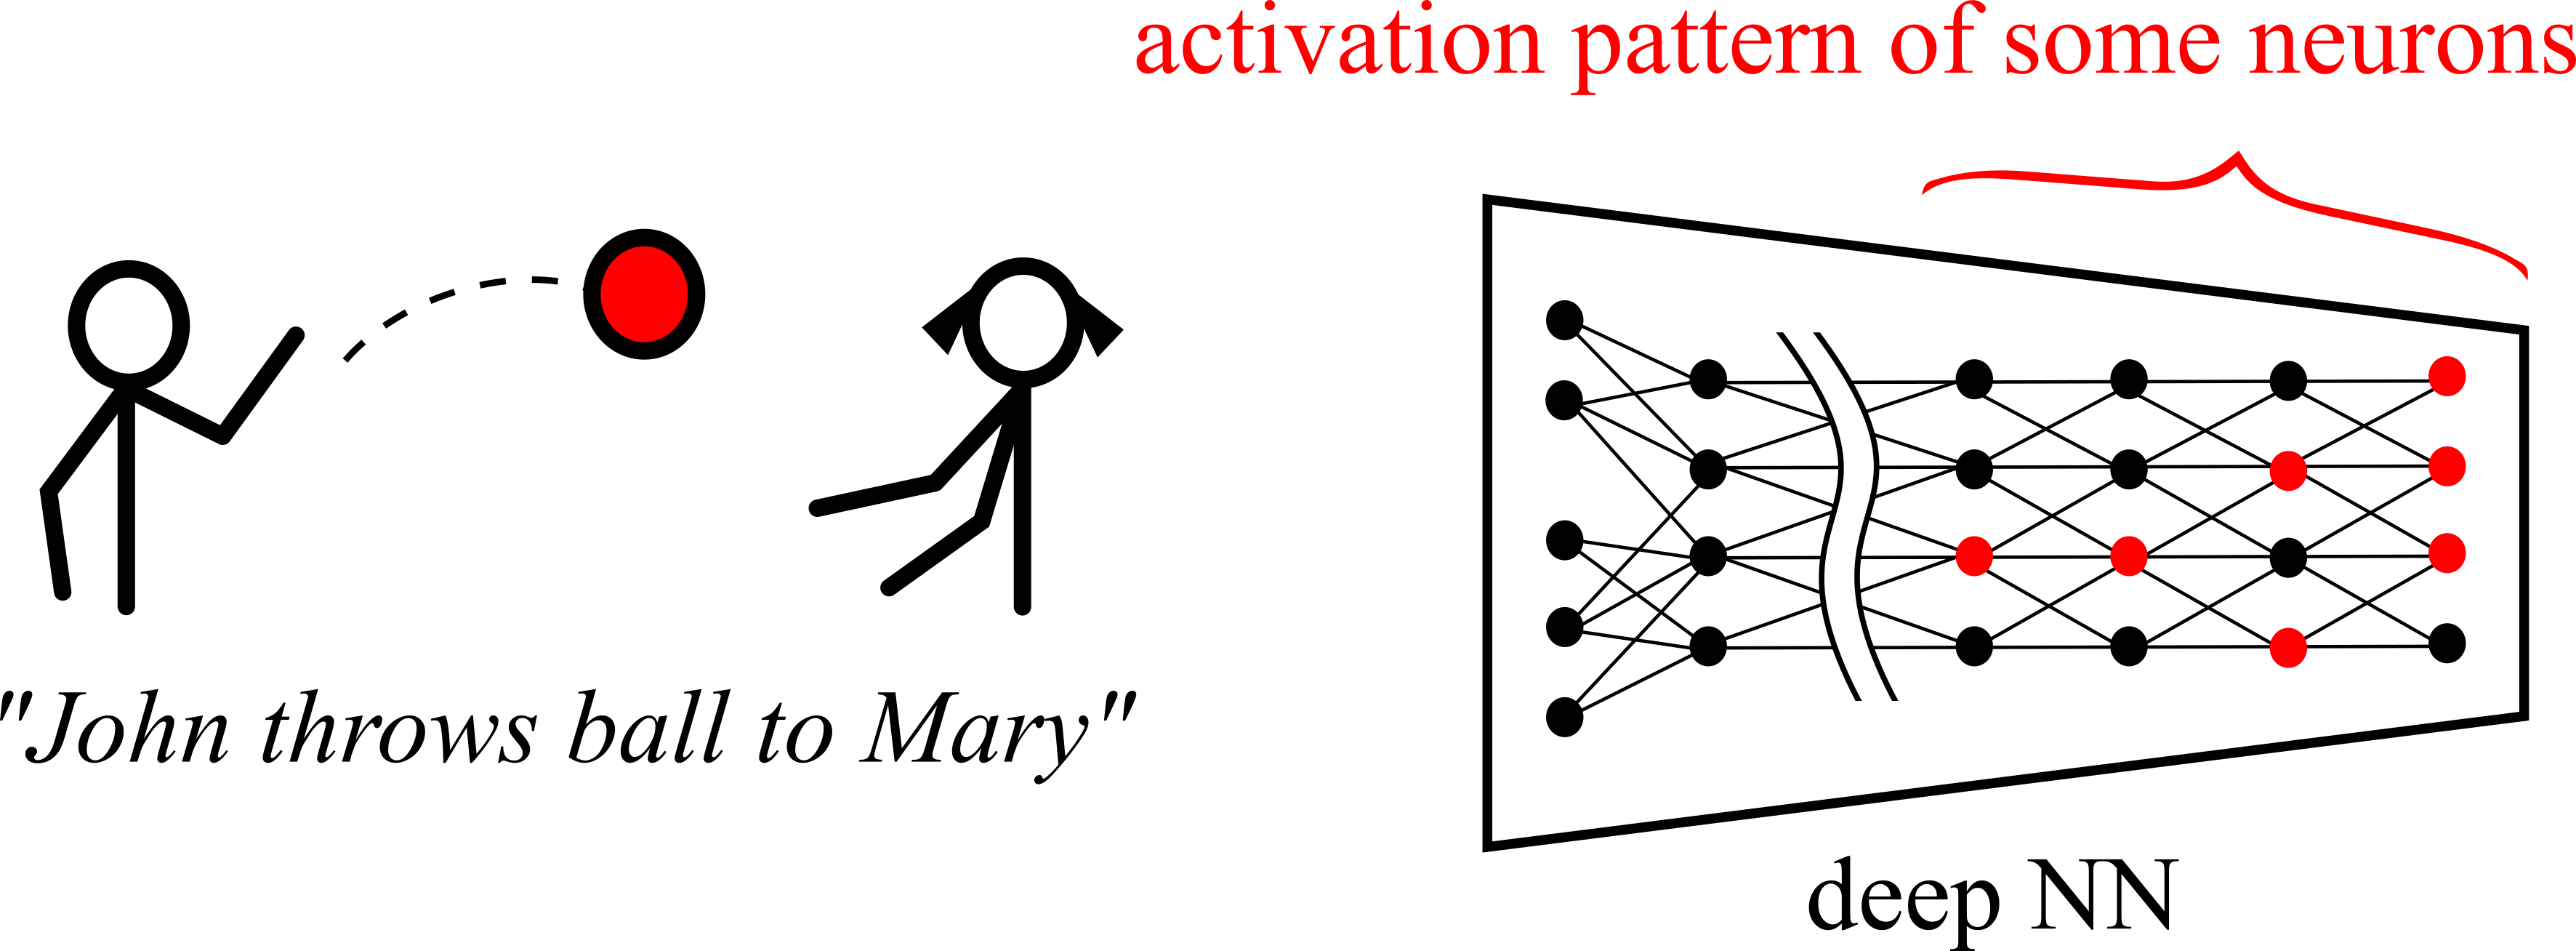
\includegraphics[scale=0.7]{NN-activation-patterns.png}}}
\end{equation}
%注意那些红点不一定是\textbf{最后}那层的输出。  这是我心目中的图像,比较 general,不是指某个特定的 implementation。  重点是: 「美女过马路」是一个 ``\textbf{neat}'' 命题,但在感知过程中,我们会认得很多细节,例如「裙子、高跟鞋、金发、斑马线、路灯」等。  这些特徵 (features) 构成整个 representation,至少我是这样理解 分布式表述 的。
\cc{这可以理解为: \uline{一个 ``neat'' 命题被分解为很多个细小的命题},例如:
}{
This can be understood as: \uline{a ``neat'' proposition is broken down into a number of small propositions}, for example:}
\begin{equation}
\mbox{A 掷球给 B} \Longleftrightarrow \left\{
                \begin{array}{l}
\cc{
                  \mbox{A手臂挥动 } \; \wedge \\
                  \mbox{球离开A的手 } \; \wedge \\
                  \mbox{球在半空飞 } \; \wedge \\
}{
                  \mbox{A flings his arm } \; \wedge \\
                  \mbox{ball leaves A's hand } \; \wedge \\
                  \mbox{ball flies in mid-air } \; \wedge \\
}
                  ...
                \end{array}
              \right.
\end{equation}
\cc{这两边是\textbf{逻辑等价}的。 在右边不能出现「球是红色的」这一细节,因为这细节不是左边\textbf{蕴涵}的。 但可以有「球通常是圆的」。 换句话说:
}{
These two sides are \textbf{logically equivalent}. The details of "The ball is red" cannot appear on the right side, because this detail is not left \textbf{implication}. But there can be "the ball is usually round". in other words:}
\begin{equation}
\boxed{\mbox{``neat'' proposition}} \quad p \Longleftrightarrow \left\{
                \begin{array}{l}
                  q_1 \; \wedge \\
                  q_2 \; \wedge \\
                  ... \; \wedge \\
                  q_n
                \end{array}
              \right.
\quad \boxed{\mbox{distributed propositions}}
\end{equation}

\cc{\textit{结论}: 未知 分布式知识表述 会给 AI 带来什么影响,暂时我们的 architectures 对 distributive 和 neat logic 同样适用,除了命题数目的增加,与及 和「视觉神经」接合 的部分。 
}{
\textit{Conclusion}: Unknown What is the impact of distributed knowledge representation on AI? For the time being, our architectures are equally applicable to distributive and neat logic, except for the increase in the number of propositions and the part of the "visual nerve".}

%经典逻辑表述是由 命题 构成的,其实 features 也可以看成是命题,例如「高跟鞋」可以看成是「有一只高跟鞋在这位置」的命题。 逻辑上来说:
%\begin{equation}
%\boxed{\mbox{neat proposition}} \quad p \Leftrightarrow \bigwedge q_i \quad \boxed{\mbox{distributive features}}
%\end{equation}
%有时(例如纯文字输入时),知道的只是一个 neat 命题,例如「美女过马路」,并不知道其他细节(例如「金发」),这时仍然可以有分布式表述,但那些特徵会是比较抽象的。

\subsection{\cc{神经网络 缺乏短期记忆}{NNs lack short-term memory mechanism}}

\cc{考虑「白猫追黑猫」这个图像:
}{
Consider the image of "White Cat Chasing Black Cat":}
\begin{equation}
\vcenter{\hbox{
\includegraphics[scale=0.6]{white-cat-chase-black-cat.png}}}
\end{equation}
\cc{「猫」的概念需要出现 \textbf{两次},但神经网络内对应於「猫」的特徵只有 \textbf{一组}(除非有两个重复的可以表示任何概念的 modules,但很浪费)。 换句话说,现时的 CNN 没有「巡迴 (traverse)」视野域的能力; \uline{它不能辨别和描述物体之间的 }\textbf{\uline{关系}}。 
}{
The concept of "cat" needs to appear \textbf{twice}, but the feature corresponding to "cat" in the neural network is only \textbf{set} (unless there are two duplicate modules that can represent any concept, but it is wasteful) . In other words, the current CNN does not have the ability to "traverse" the field of view; \uline{it cannot distinguish and describe the }\textbf{\uline{relationships}}\uline{ between objects.}}

\cc{很难想像一个 ``monolithic'' neural module (例如 feed-forward NN 或 RNN)怎样可以做到这功能。 似乎必须将命题表述成一连串 概念 的 \textbf{时间序列} (time sequence),即某种 \textbf{短期记忆} (\textbf{STM}, short-term memory)。
}{
It's hard to imagine how a ``monolithic'' neural module (such as feed-forward NN or RNN) can do this. It seems necessary to express the proposition as a series of concepts of \textbf{time sequence}, some kind of \textbf{short-term memory} (\textbf{STM}, short-term memory).}

\cc{我有点惊讶地发现,目前 神经网络 没有 \textbf{短期记忆} 的机制,「短期」意思是在 time-scale 上短於 weights 改变的时间。 例如我告诉你一串数字(例如电话号码),你可以在脑中记住它,但这个机制在现时人工神经网络里面似乎没有研究,或许在 computational neuroscience 里面有些模型,但暂时我不清楚。  缺乏这种 STM,则很难模拟 symbolic logic,换句话说,做不到强人工智能。 
}{
I was a little surprised to find that the current neural network does not have the mechanism of \textbf{short-term memory}, and "short-term" means that the time-scale is shorter than the time when the weights change. For example, I tell you a string of numbers (such as a phone number), you can remember it in the brain, but this mechanism seems to have no research in the current artificial neural network, perhaps some models in computational neuroscience, but for the time being I don't know. Without such an STM, it is difficult to simulate symbolic logic. In other words, strong artificial intelligence cannot be achieved.}

\cc{例如用 NN 实现一个 \textbf{动态的记忆体},它接收新来的元素时,会对记忆体中其他元素逐一 \textbf{比较},而且具备 \textbf{复制} 功能。  例如以下这个像「迴转木马」的时间序列机制(每个 $\NewSym{distributive-vector.png}$ 代表一支 distributive vector):
}{
For example, using NN to implement a \textbf{dynamic memory}, when it receives a new element, it will \textbf{compare} to other elements in the memory, and it has the \textbf{copy} function. For example, the following time series mechanism like "Rotating Trojan" (each $\NewSym{distributive-vector.png}$ represents a distributive vector):}
\begin{equation}
\vcenter{\hbox{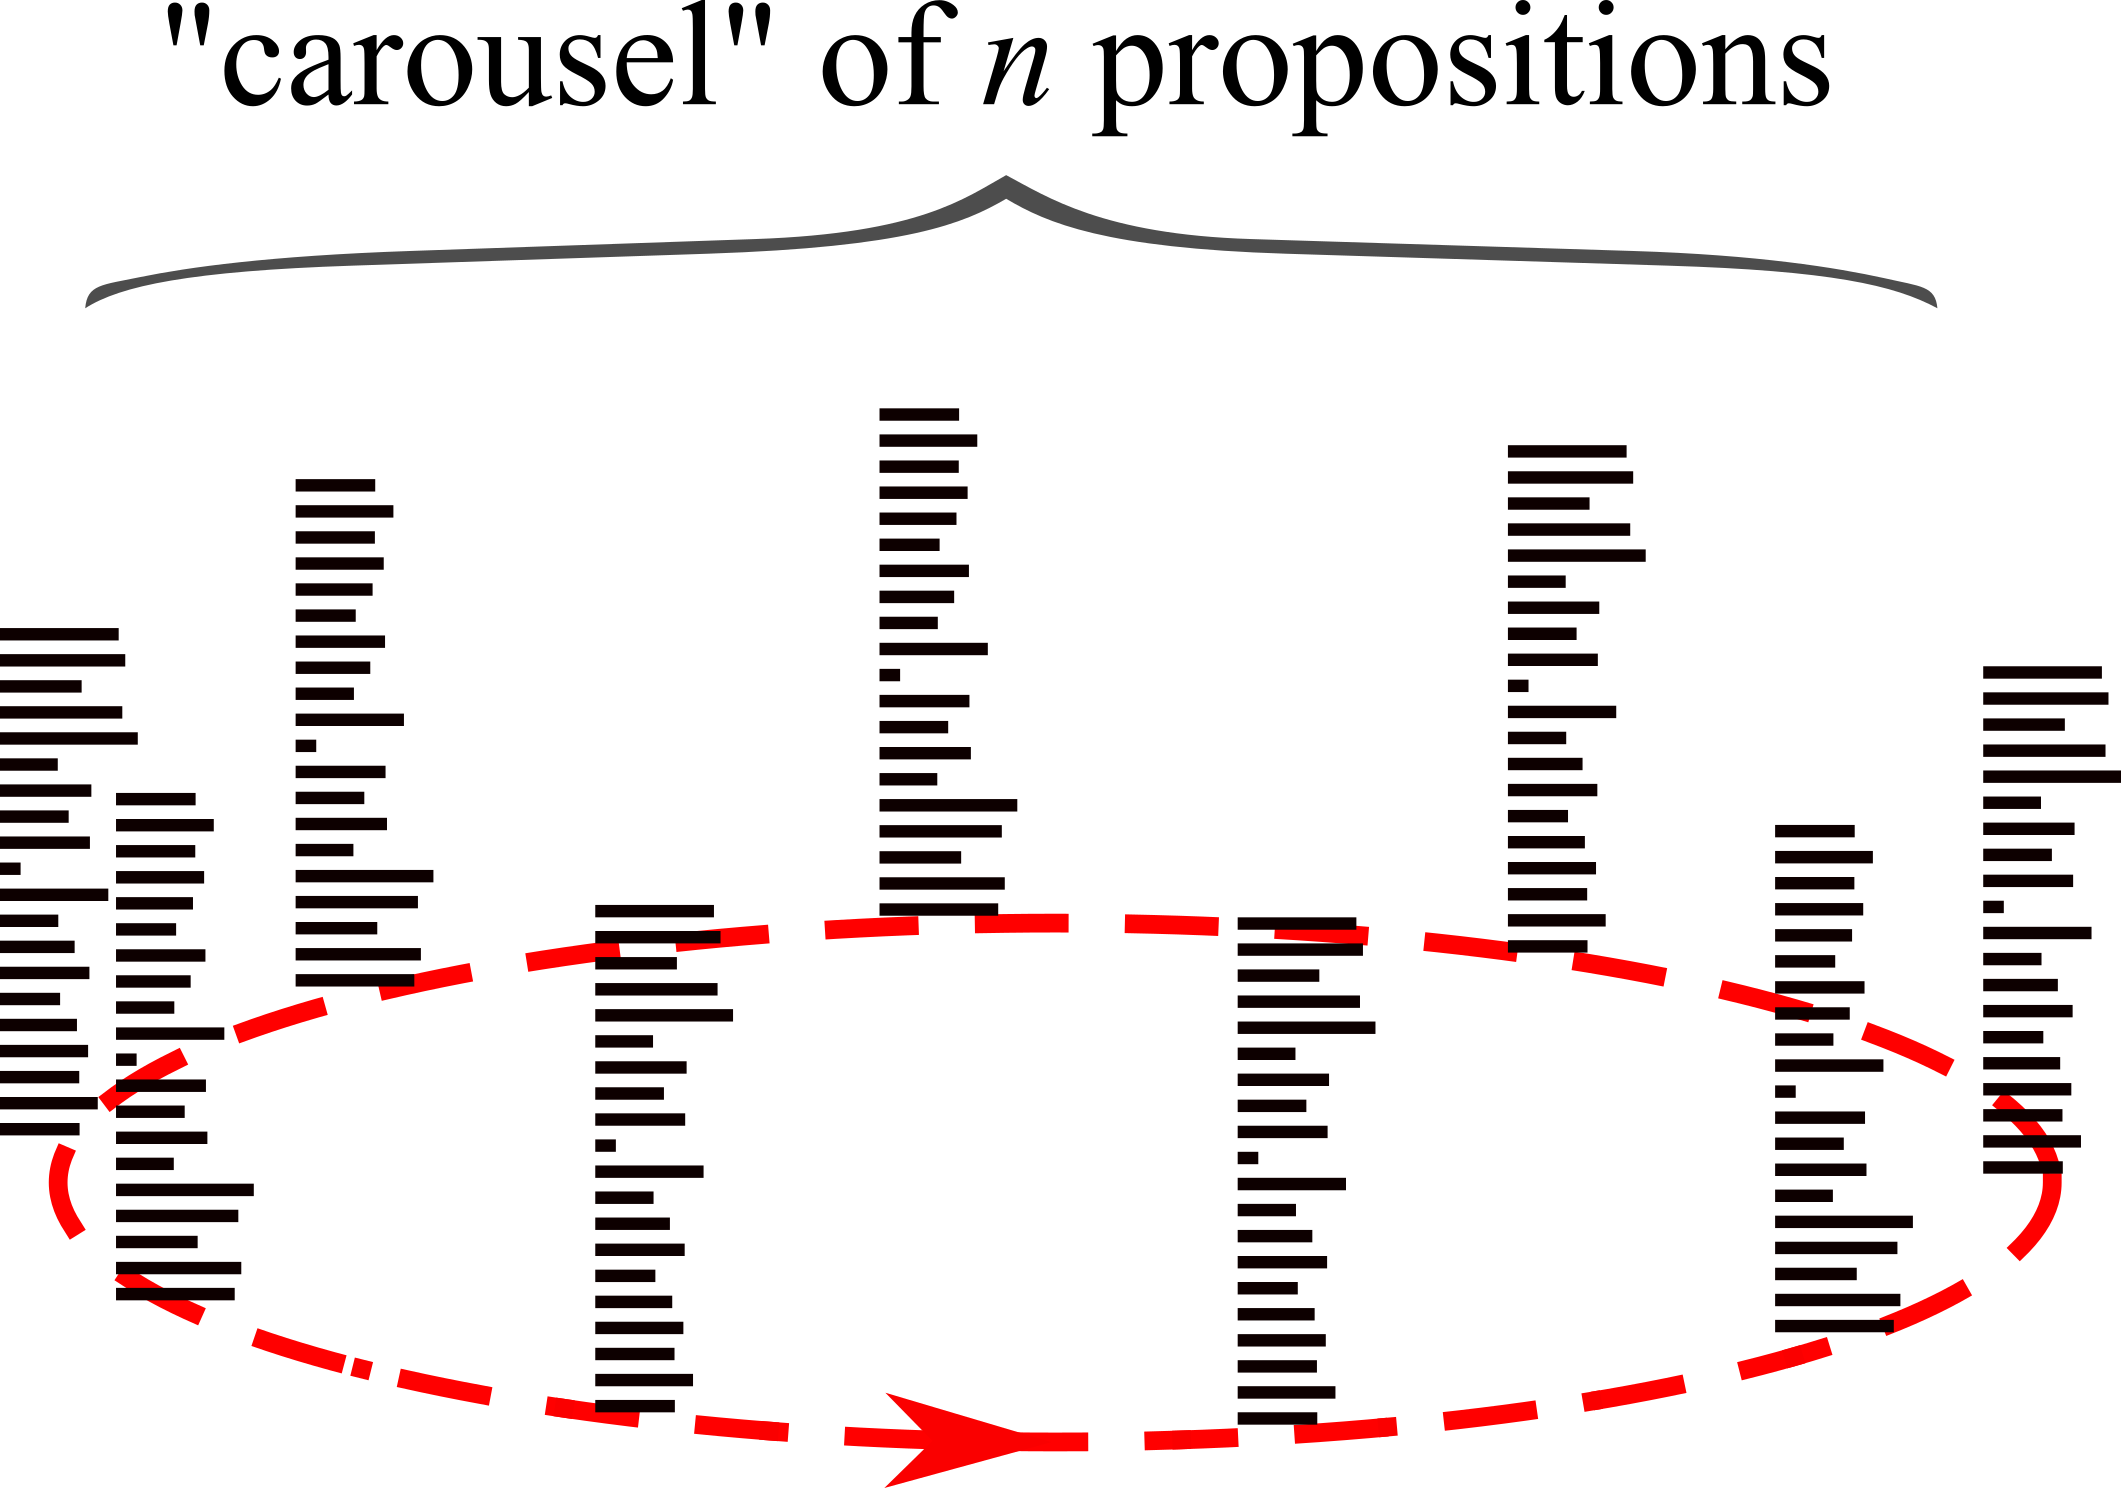
\includegraphics[scale=0.7]{carousel-of-vectors.png}}}
\end{equation}
\cc{总之,纯粹用 NN 模拟 STM,明显地很麻烦。
}{
In short, it's obviously cumbersome to simulate STM purely with NN.}

%\begin{tcolorbox}[breakable, colback=yellow]
%用神经网络解决强人工智能的最大障碍是 从命题逻辑到一阶逻辑的\textbf{跃升},特别是 substitution 运算,需要有 short-term memory 机制
% The bottleneck of strong AI is the \textbf{learning algorithm}'s speed, and the most crucial obstruction is the \textbf{lifting} from propositional to first-order logic.
%\end{tcolorbox}

\subsection{Graph NNs}
\label{graph-NN}

\begin{tcolorbox}[ams equation, colback=yellow, colframe=white]
\cc{
\mbox{用 graph 做记忆体(包括短期和长期记忆)}}{
\begin{aligned}
\mbox{Use a \textbf{graph} for memory storage} \\
\mbox{(including long-term and short-term memories)}
\end{aligned}
}
\end{tcolorbox}
\cc{而在增加新记忆单元时,相同的 nodes 会被 match 成一个,换句话说 matching 这步骤用传统 symbolic 方法解决,馀下的问题再交给 神经网络。 
}{
When adding a new memory unit, the same nodes will be matched into one. In other words, the matching step is solved by the traditional symbolic method, and the problem is left to the neural network.}
\begin{eqnarray}
\mbox{model } \mathscr{M} &=& \mbox{graph} \nonumber \\
\mbox{rewriter} &=& \mbox{deep NN = graph neural network}
\end{eqnarray}

\cc{很多谢 Google / DeepMind 在 2018 年 6 月发表的 graph network 论文 \parencite{Battaglia2018},Peter Battaglia 和 26 名合作者 survey 了 graph network 的发展情况。  他们提出的 graph network 更接近一些 physical system 例如 弹簧和球体 的系统,而不是 first-order 的模型,但本质上是一样的。
}{
Many thanks to the graph network paper \parencite{Battaglia2018} published by Google / DeepMind in June 2018, Peter Battaglia and 26 collaborators surveyed the development of graph network. The graph network they proposed is closer to some physical systems such as springs and spheres, rather than the first-order model, but essentially the same.}

\cc{通常 model 太大,需要用 attention mechanism 选取它的一个 fragment,再 ``present'' 给 神经网络 处理:
}{
Usually the model is too large, you need to use the attention mechanism to select a fragment of it, and then ``present'' to handle the neural network:}
\begin{equation}
\vcenter{\hbox{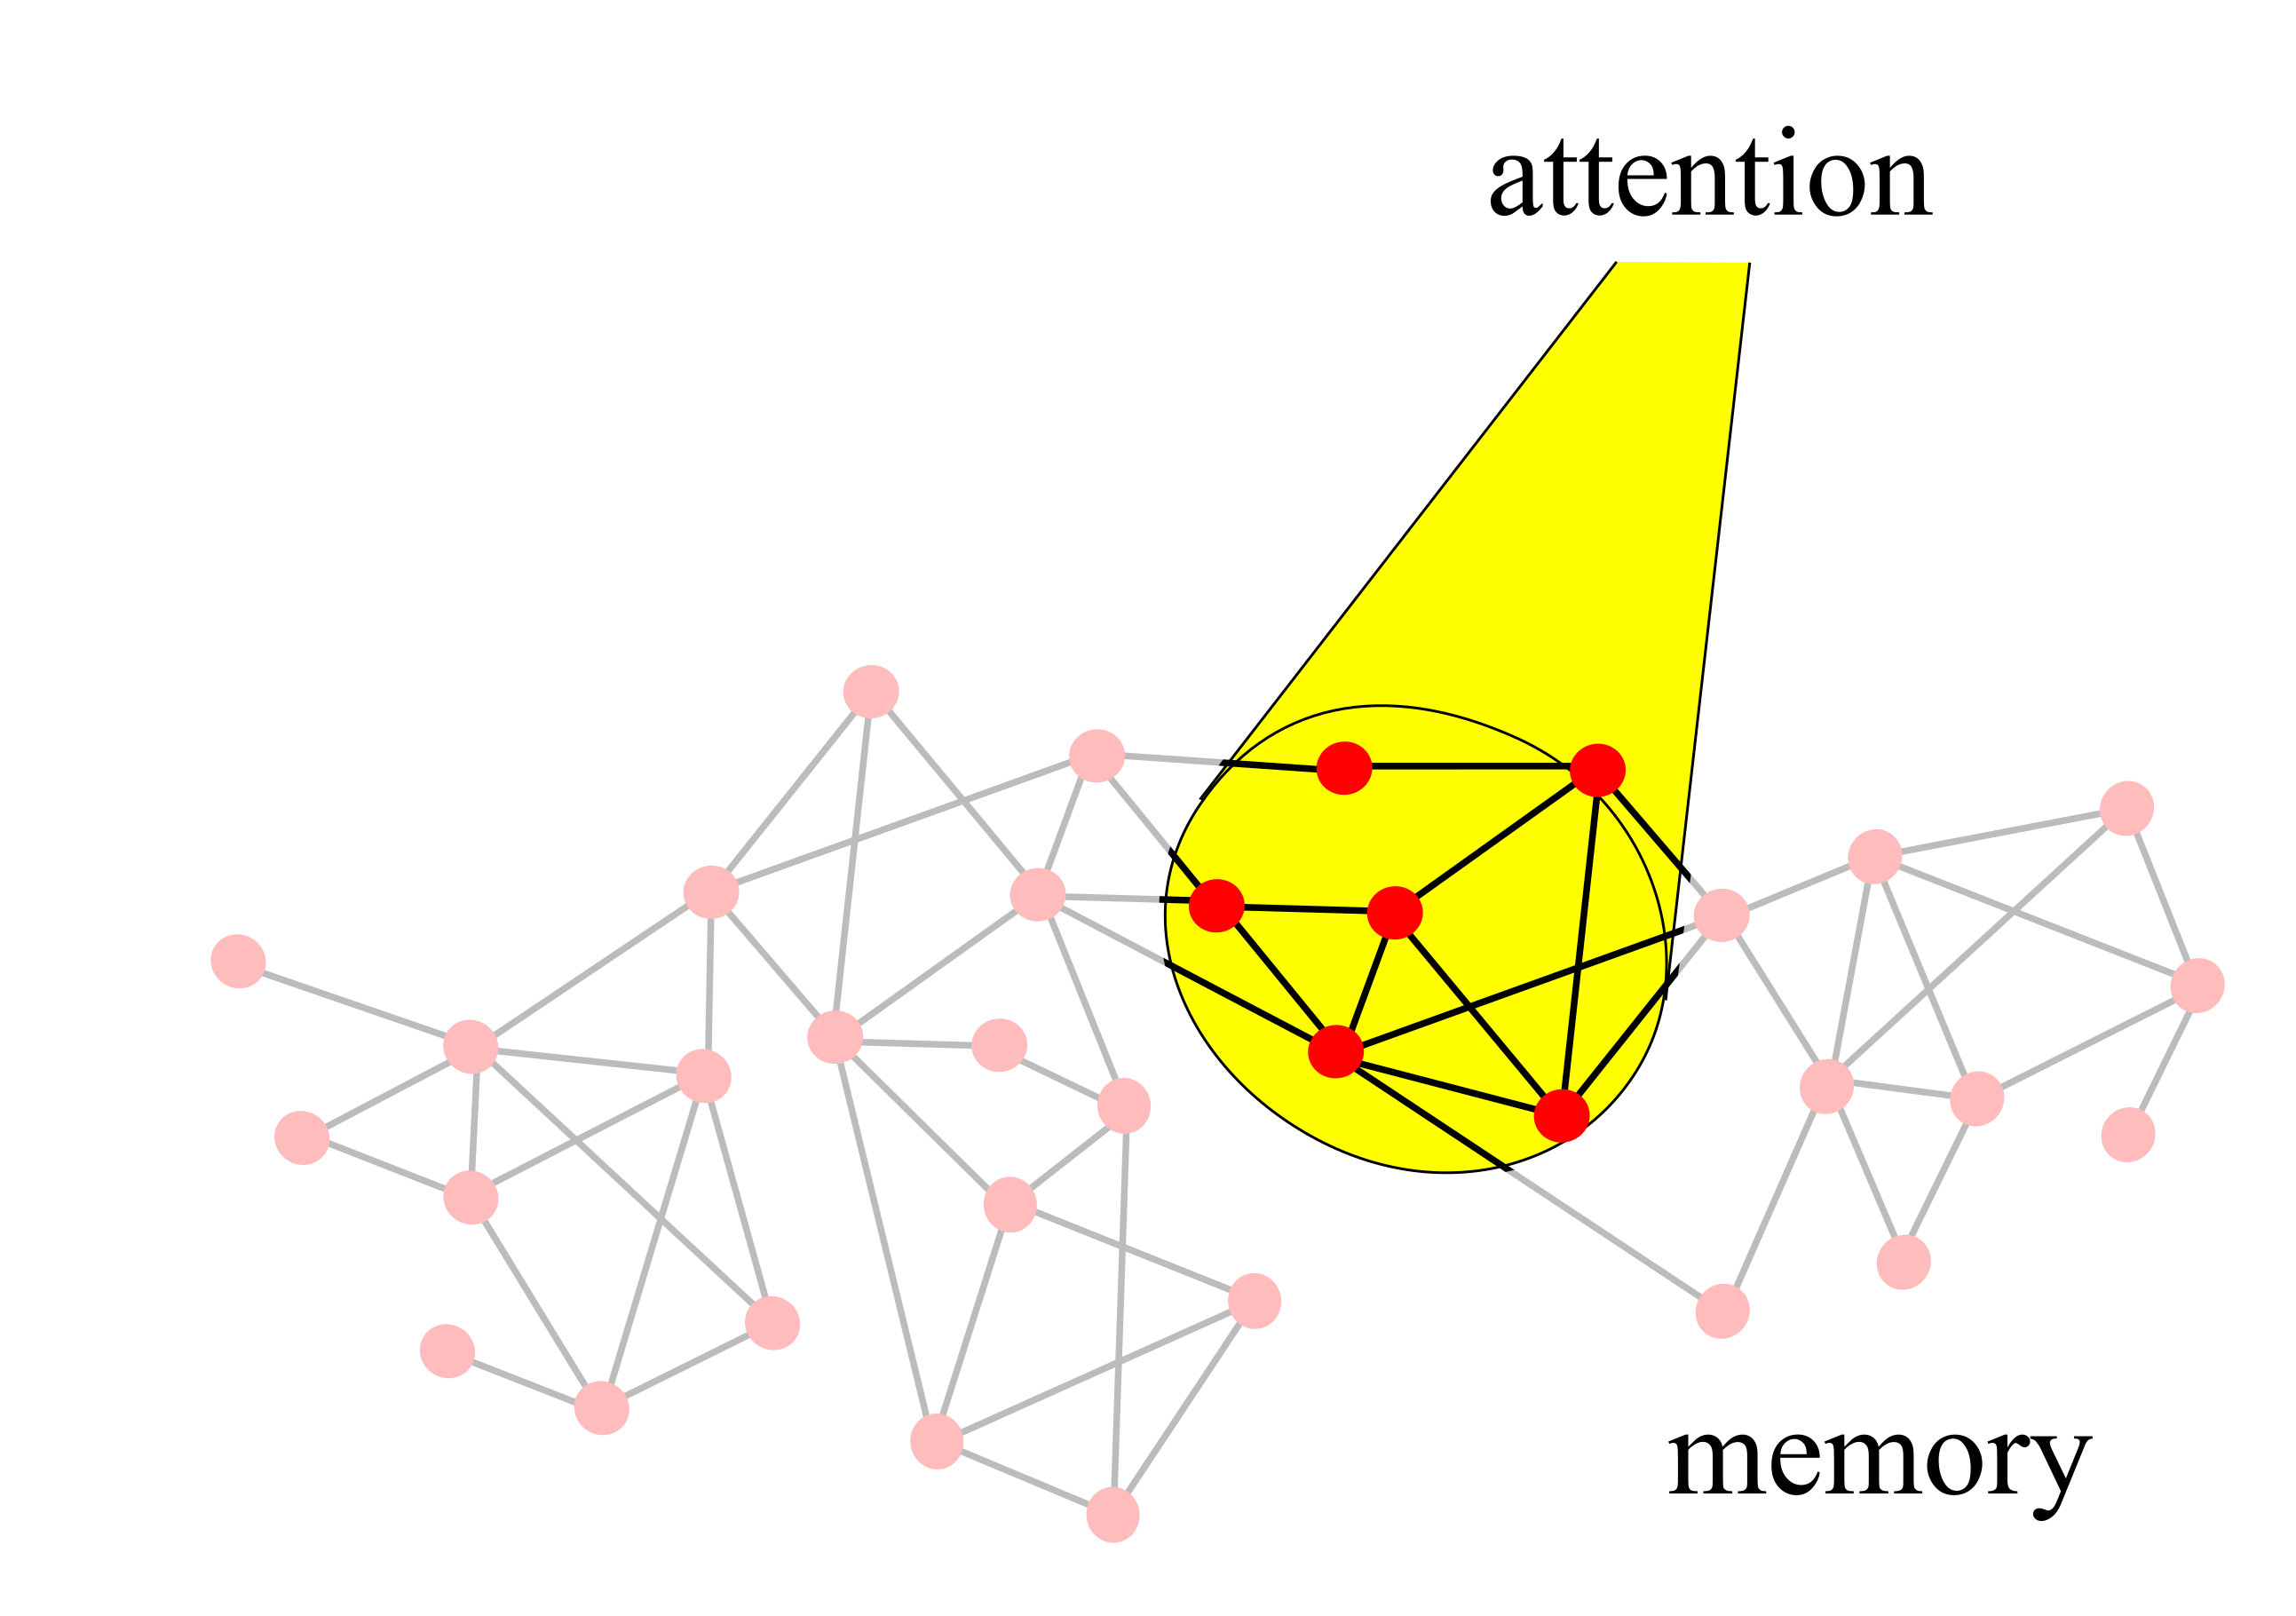
\includegraphics[scale=0.7]{attentional-mechanism.png}}}
\end{equation}
\cc{这 attention mechanism 和 现时 深度学习 里面的 attention 或者在具体细节上有些分别,但基本上是同一概念。 
}{
This attention mechanism is somewhat different from the attention in the current deep learning or in the specific details, but basically the same concept.}

\cc{神经网络的输入 $\vec{x}$,需要这样的一个 embedding:
}{
The neural network input $\vec{x}$ requires an embedding like this:}
\begin{equation}
\boxed{\mbox{graph}} \quad
\begin{tikzcd}[column sep = large]
\NewSym[1.5]{../graph-symbol.png} \ar[r, hookrightarrow, "\mbox{embed}"] & (x_1, ..., x_m) 
\end{tikzcd}
\quad \boxed{\mbox{vector}}
\end{equation}
\cc{但 graph 并不是一个「线性」的结构 \footnote{线性是指符号形式上,例如 tree 可以表示成线性的一行},将 graph 结构表示成一支 vector 似乎颇难(这或许是 graph neural networks 迟迟未有突破的原因)。  
}{
But graph is not a "linear" structure \footnote{linear means symbolic form, for example, tree can be represented as a linear line}, it seems quite difficult to represent the graph structure as a vector (this may be the delay of the graph neural networks) There are reasons for the breakthrough).}

\begin{tcolorbox}[breakable, parbox=false, fonttitle=\bfseries, title=Quiver representations]
\cc{数学表示论里面有 \textbf{quiver representations},它将 vertex 变成 vector space,edge 变成 linear transformation between vector spaces. 例如:
}{
In representation theory one studies \textbf{quiver representations}, which turns \textbf{vertices} into vector spaces and \textbf{edges} into linear transformations between vector spaces.  For example:}
\begin{equation}
\begin{tikzcd}[column sep = large]
\mbox{John} \arrow[r, bend left, "\heartsuit"] & \arrow[l, bend left, swap, "\neg \heartsuit"] \mbox{Mary}
\end{tikzcd}
\quad \Longrightarrow \quad
\begin{tikzcd}[column sep = large]
V_1 \arrow[r, bend left, "M_1"] & \arrow[l, bend left, "M_2"] V_2
\end{tikzcd}
\end{equation}
\cc{其中 $V_1, V_2$ 是向量空间,$M_1, M_2 \in GL(\mathbb{R})$ 是 矩阵。
}{
where $V_1, V_2$ are vector spaces, $M_1, M_2 \in GL(\mathbb{R})$ are matrices.}

The vector spaces $V_i$ can be \uline{stacked up vertically} to form a single big vector space $V$.  Then all the relations fit into an endomorphism $V \rightarrow V$.

\cc{在 向量空间 $V_i$ 的 \textbf{基底变换}下,两个矩阵 $M$ 和 $M'$ 可能是同一个线性变换。  故需要考虑它们的\textbf{不变性},亦即 moduli。 表示论 关心的是 将各种 $M$ \uline{分解成不可约成分}。 这分解里出现的 Dynkin diagrams 和 Lie algebra 分类时出现的一样。  但如果 quiver 不是 Dynkin 或某些扩充,则这 quiver 是 ``wild'' 的,很难分解。 即使很简单的 quiver 也可以是 wild type。
}{
Under \textbf{change of basis} of the vector spaces $V_i$, two matrices $M$ and $M'$ may turn out to be the same linear transformation. Therefore, we need to consider their \textbf {invariant form} or \textbf{moduli}. Representation theory is concerned with the decomposition of $M$ \uline{into irreducible components}. The \textbf{Dynkin diagrams} that arise in this decomposition are the same as those found in Lie algebra classification.  If the quiver is not a Dynkin diagram then the quiver is ``wild'' and is generally difficult to study.  Even a simple quiver can be of wild type.}

\cc{每个 quiver 定义一个 path algebra,它的元素是 quiver 里的 path,换句话说即是逻辑上的 \textbf{关系} 及其 compositions。
}{
Each quiver defines a \textbf{path algebra} whose elements are the paths in the quiver.  In logic these paths correspond to logical \textbf{relations} and their composition.}
\end{tcolorbox}

\cc{整体运作是这样的:
}{
The overall operation is like this:}
\begin{equation}
\vcenter{\hbox{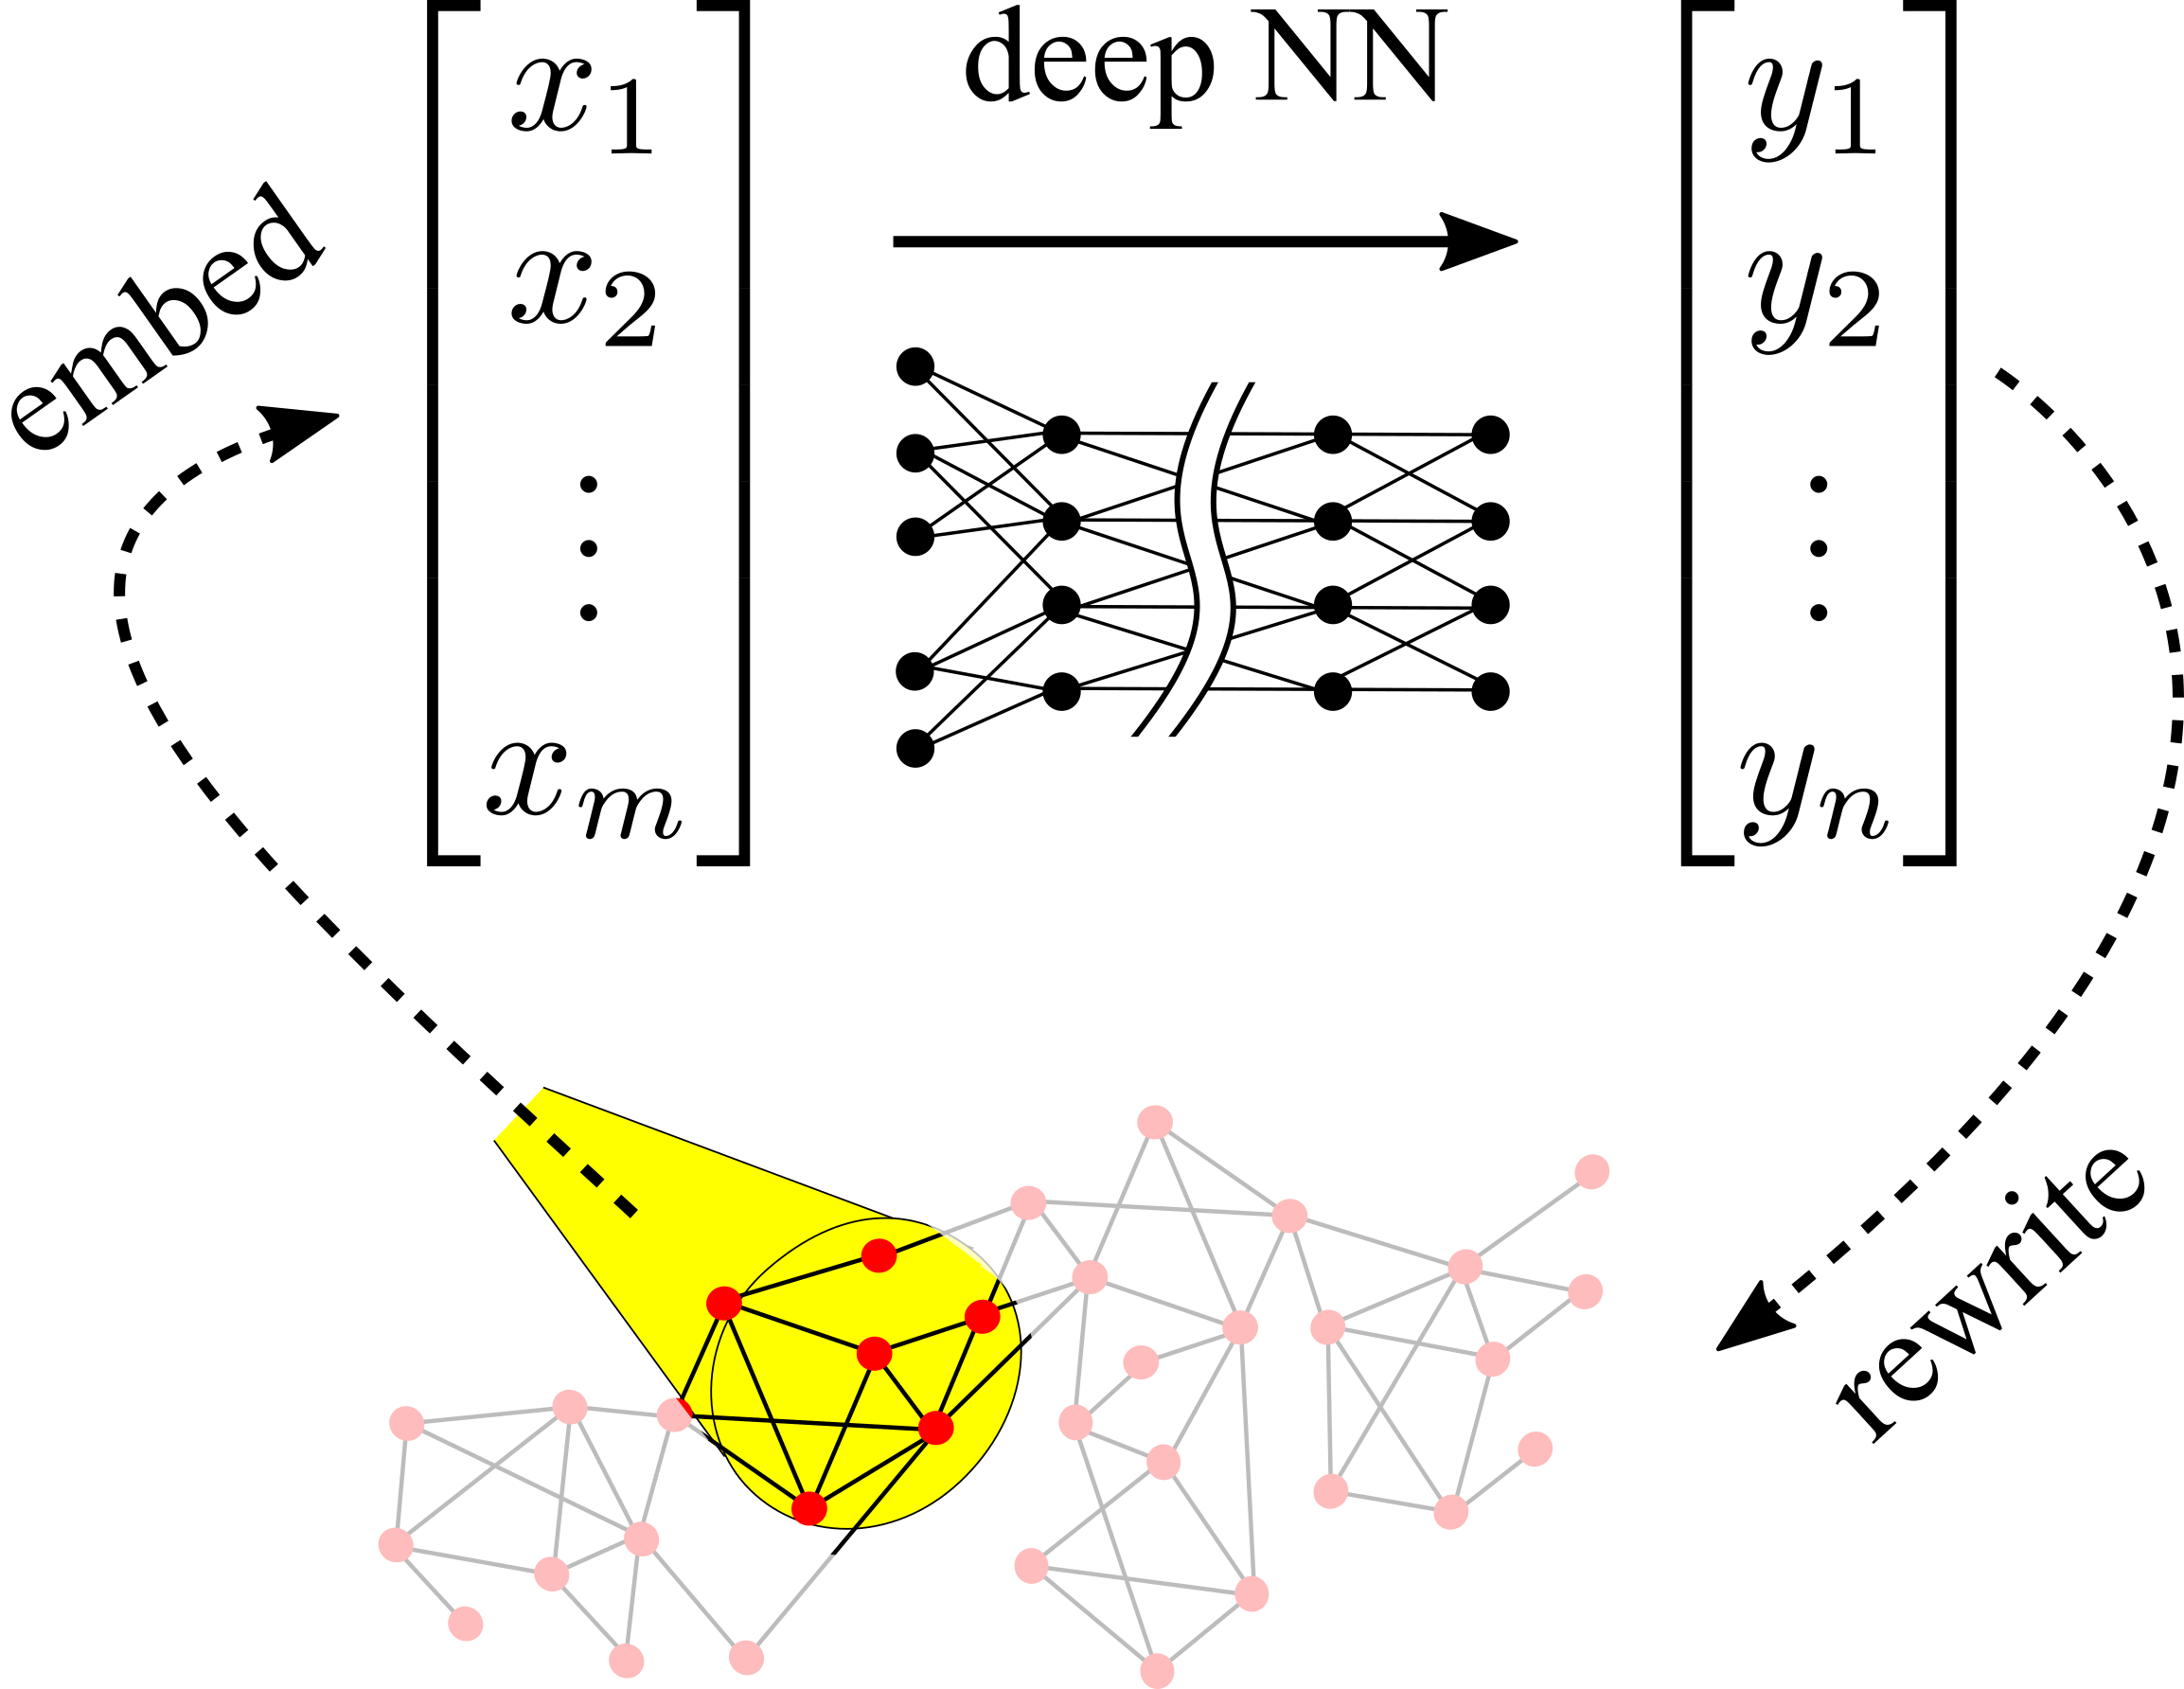
\includegraphics[scale=0.6]{graph-NN-rewriting.png}}}
\end{equation}
\cc{这 deep NN 可以是 CNN 或 RNN,因为它们现时 在 自然语言理解/翻译 方面 很成功,但它们处理的是线性的 sequence 输入。 或者可以将 memory sub-graph 分拆成线性的元素(亦即个别的 关系/命题),而且里面不可以用 global variable references(换句话说,已经进行了 variable matching 处理)。  然后 NN 输出的 variable copying 也是 externally 处理的。 换句话说,用 ``hybrid'' 的方式,结合 NN 和 \textbf{graph rewriting}。  图中那 embedding 细节目前我仍未见过良好的解决办法,但 DeepMind / Google 他们的研究已经很接近了。
}{
This deep NN can be either CNN or RNN because they are currently very successful in natural language understanding/translation, but they deal with linear sequence inputs. Or you can split the memory sub-graph into linear elements (that is, individual relationships/propositions), and you can't use global variable references (in other words, variable matching has been done). Then the variable copying output by NN is also externally processed. In other words, in combination with NN and \textbf{graph rewriting} in the ``hybrid'' way. I still haven't seen a good solution for the embedding details in the picture, but DeepMind / Google's research is very close.}

\cc{注意: 虽然 NN 的参数空间 $\Theta \in \mathbb{R}^N$ 是 \textbf{连续}的,但它 learn 出来的 rewriting rules 却是 \textbf{离散}的,因为 graph 本身是个 离散结构。 
}{
Note: Although the parameter space $\Theta \in \mathbb{R}^N$ of NN is \textbf{continuous}, the rewriting rules it learns are \textbf{discrete} because graph itself is a discrete structure. .}

\cc{补充一点: attention mechanism 要 traverse memory graph,换句话说是一种 graph search algorithm,这部分可以和 NN 结合成同一个 module(现时有很多 RNN architectures 就是这样)。
}{
Add a point: attention mechanism to traverse memory graph, in other words a graph search algorithm, this part can be combined with NN into the same module (there are many RNN architectures now).}

\begin{center}
\rule{0.4\textwidth}{.6pt}
\end{center}
\cc{馀下 2 节是一些 数学 背景知识....
}{
The rest of this paper are some background mathematical knowledge...}

\section{What is topos theory?}
\label{topos}

\cc{\uline{Topos 可以理解为 set theory 受范畴论影响下的一种推广}。 每个 elementary topos\footnote{Elementary 是集合中「元素」的意思} 有一个 \textbf{sub-object classifier} $\Omega$.  $\Omega$ 是一个特殊的 object,例如 $\{ \top, \bot \}$,代表 \textbf{真 假} 二值。 用 $\Omega$ 可以定义 sub-objects 亦即集合论中的 \textbf{子集} 概念。  举例来说,``Love'' 是一个在 $D \times D$ 内的 \textbf{关系},$D$ 是所有「人」的集合。  可以将 $D \times D$ 看成是 full relation,则 $\mbox{Love} \subset D \times D$ 是它的\textbf{子集}。  换句话说,这是 elementary topos 可以用来做 relation algebra 或 first-order logic 的 \textbf{模型} 的原因。 (参见 \parencite{Goldblatt1984})
}{
\uline{Topos theory can be understood as a generalization of set theory under the influence of category theory}.}

An \textbf{elementary topos} (``elementary'' as in ``elements'' of a set) is a \textbf{Cartesian-closed category} (CCC) with a \textbf{sub-object classifier} $\Omega$.

A Cartesian-closed category is, roughly speaking, where one can form arbitrary:
\begin{itemize}
\item  \textbf{Cartesian products} $A \times B$, and
\item  \textbf{exponentiation} $B^A$
\end{itemize}
where $B^A \simeq A \rightarrow B$ is the class of all functions from $A$ to $B$.

The sub-object classifier $\Omega$ allows a topos to handle \textbf{subsets} as in set theory.  In the category $\mathbf{Set}$, $\Omega$ is $\{ \top, \bot \}$, representing True and False.  

For example, ``Love'' is a \textbf{relation} within $D \times D$, where $D$ is the universe set of all ``people''.  One can think of $D \times D$ as the ``full'' relation, then $\mbox{Love} \subset D \times D$ is its \textbf{subset}.  Thus sub-objects enable elementary toposes to model relation algebra and first-order logic.  A standard textbook on topos theory is \parencite{Goldblatt1984}.

\subsection{Some history}

\cc{「\textit{Lawvere 和 Tierney 发展的 elementary topoi 理论\footnote{around 1960-70},是 categorical algebra 历史上最重要的事件.....  这不只是他们证明了这些东西,而是他们敢於相信这是可能的}」--- Peter Freyd.
}{
\textit{``The development of elementary topoi by Lawvere and Tierney [around 1960-70] strikes this writer as the most important event in the history of categorical algebra since its creation..... It is not just that they proved these things, but that they dared to believe them provable.'' --- Peter Freyd.}}

\textit{``In a sense logic is a special case of geometry.'' --- Bill Lawvere.}

\cc{在 1963 年左右,topos 的概念独立地来自几个不同的发源地: Alexander Grothendieck 在代数几何方面发展的 sheaf theory,和 F William Lawvere 用范畴论重新表述集合论,还有 Paul Cohen 的 forcing 理论(后者用来解决 \textbf{连续统假设})。  Sheaf 的意思是: 在一些 open sets $V_i$ 上定义的物体,它们在 overlap $V_i \cap V_j$ 上是吻合的,即可以 ``collate'',情形就像微分几何里一些 charts 拼合成 atlas。  二战后,Leray,接著 Cartan,用 open sets 的方法定义了 sheaf。 其后 Lazard 用 \'{e}tale 定义 sheaf,后者是 topos 理论的主要动机。  例如,一个范畴 $\mathscr{A}$ 上的 pre-sheaf 可以定义为一个 \textbf{functor}:
}{
Around 1963, the concept of topos came independently from several different sources:

\begin{itemize}
\item Alexander Grothendieck's sheaf theory in algebraic geometry

\item F William Lawvere's categorical re-formulation of set theory

\item Paul Cohen's invention of forcing (to resolve the \textbf{Continuum Hypothesis})
\end{itemize} 

A useful aspect of topos theory is that it allows for a great variety of different \textbf{models} in contrast to ZFC for which it is fairly hard to construct different models.  Thus topos theory helped Cohen to construct forcing models for ZFC where the Continuum Hypothesis fails.

Sheaf means: Objects defined on some open sets $V_i$, they are consistent on the overlap $V_i \cap V_j$, which can be ``collate''. The situation is like some charts in differential geometry. . After World War II, Leray, then Cartan, defined sheaf using the open sets method. Later Lazard defined sheaf with \'{e}tale, which is the main motivation for the topos theory. For example, a pre-sheaf on a category $\mathscr{C}$ can be defined as a \textbf{functor}:}
\begin{equation}
\widehat{\mathscr{C}}: \mathscr{C}^{\mathrm{op}} \rightarrow \mathbf{Set}
\end{equation}
\cc{亦即是 范畴 $\mathscr{C}$ 上的一「层」set-valued functions.  它是 ``functor'' 所以处理了那些 collating.  这个 functor 是 contravarient 所以有 $\mathrm{op}$.  Grothendieck 将 sheaf 应用在 topology (cohomology)上,而后 Jean-Pierre Serre 发现它也可以用在代数几何上,他们和其他合作者 写了 1623 页的巨著 《SGA IV》,重大影响了代数几何的发展,导致 1974 年 Deligne 解决了 Weyl 猜想。  但我暂时不熟悉代数几何,所以不太清楚 Grothendieck 他们做了什么.... 详细可参看 \parencite{MacLane1992} 一书。
}{
That is, a "layer" set-valued function on the category $\mathscr{C}$. It is ``functor'' so it handles those collating. This functor is contravarient so there is $\mathrm{op}$. Grothendieck Applying sheaf to topology (cohomology), then Jean-Pierre Serre found that it can also be used in algebraic geometry. They and other collaborators wrote the 1623-page masterpiece "SGA IV", which greatly influenced the development of algebraic geometry, resulting in In 1974 Deligne solved the Weyl conjecture. But I am not familiar with algebraic geometry for the time being, so it is not clear what Grothendieck did.... See the book \parencite{MacLane1992} for details.}

\cc{在拓樸空间上,一个 open set $U$ 的 complement 是 closed 而且未必 open,所以如果局限在 open sets 之内,则 $U$ 的 ``negation'' 应该定义为 ``the interior of its complement''.  这导致 $U$ 的「\textbf{双重否定}」不一定等於 $U$,换句话说,\uline{the algebra of open sets follows \textbf{intuitionistic logic}}, such an algebra is called a \textbf{Heyting algebra}.  (参考书同上)
}{
In the topology space, the complement of an open set $U$ is closed and not necessarily open, so if it is confined within the open sets, the ``negation'' of $U$ should be defined as ``the interior of its complement' '. This causes $U$'s "\textbf{double negative}" not necessarily equal to $U$, in other words, \uline{the algebra of open sets follows \textbf{intuitionistic logic}}, such an algebra is called a \textbf{Heyting algebra}. (cf. ibid.)}

\cc{Topoi 之间有两种 morphisms: \textbf{geometric morphisms} 和 \textbf{logical functors}.  前者保持「几何结构」,后者保持逻辑上的 type theory,所以有 \textbf{elementary topos} 的定义。 后者的特点是它有 \textbf{sub-object classifier} $\Omega$。 
}{
There are two kinds of morphisms between Topoi: \textbf{geometric morphisms} and \textbf{logical functors}. The former maintains "geometry", the latter maintains a logical type theory, so there is a definition of \textbf{elementary topos}. The latter is characterized by its \textbf{sub-object classifier} $\Omega$.}

\subsection{Sub-object classifier}

This commutative diagram defines the sub-object classifier $\Omega$:
\begin{equation}
\begin{tikzcd}[column sep = large, row sep = large]
A \arrow[r, hook, "f"] \arrow[d, swap, "!"]  \arrow[dr, phantom, "\lrcorner", very near start]
	& D \arrow[d, "\Chi_f"] \\
1 \arrow[r, "true"] & \Omega
\end{tikzcd}
\end{equation}

Pulling $true$ back along $\Chi_f$ yields the set $\{ x: \Chi_A(x) = 1 \}$ which is just $A$.

The arrow $\Chi$ is called the \textbf{classifying} arrow of the sub-object $A$;  It can be thought of as taking exactly the part of $D$ that is $A$ to the ``point'' $t$ of $\Omega$.

We form a collection, the sub-objects of $D$:
\begin{equation}
\mathrm{Sub}_{\mathscr{C}}(D) = \{ [f]: f \mbox{ is a monic with } \mathrm{cod} f = D \}
\end{equation}

If $\mathscr{C}$ has pullbacks (of monomorphisms along arbitrary morphisms in $\mathscr{C}$) then $\mathrm{Sub}_{\mathscr{C}}(D)$ extends to a functor $\mathrm{Sub}_{\mathscr{C}}: \mathscr{C}^{\mathrm{op}} \rightarrow \mathbf{Set}$ by putting $\mathrm{Sub}_{\mathscr{C}}(f)([m]_\sim) = [f^* m]_\sim$  where $f^* m$ is the pullback of $m$ along $f$. {\color{red}(??)} \parencite{Streicher2006} p.79.

The pullback condition is equivalent to requiring the contra-variant sub-object functor,
\begin{equation}
\mathrm{Sub}_{\mathscr{C}}(-): \mathscr{C}^{\mathrm{op}} \rightarrow \mathbf{Sets}
\end{equation}
(which acts by pullback) to be \textbf{representable}, ie:
\begin{equation}
\mathrm{Sub}_{\mathscr{C}}(-) \cong  \mathrm{Hom}_{\mathscr{C}}(-, \Omega).
\end{equation}
The required isomorphism is just the pullback condition stated in the definition of a sub-object classifier \parencite{Awodey2006} p.175.

A contra-variant (or co-variant) presheaf $F: \mathscr{C}^{\mathrm{op}} \rightarrow \mathbf{Set}$ is called \textbf{representable} if it is isomorphic to $\mathrm{Yon}_{\mathscr{C}}(I) = \mathscr{C}(-, I)$ (or $\mathscr{C}(I, -)$) for some $I \in Obj \; \mathscr{C}$.

\textbf{Example.}  If $\mathscr{C}$ is a monoid M (considered as a category) then $\Omega$ consists of all right ideals in $M$, \textit{ie}, subsets $I$ of $M$ such that $x \in I$ and $y \in M$ implies $xy \in I$, and $\Omega(x)(I) = \{ y \in M | xy \in I \}$. \parencite{Streicher2006} p.83. {\color{red}(??)}

\textbf{Example.}  If $\mathscr{C}$ is a group then according to the above example, the truth value object $\Omega$ of the topos $\widehat{\mathscr{C}}$ of $G$-actions has $\{ G, \varnothing \}$ as underlying set because $G$ and $\varnothing$ are the only right ideals in $G$ which, moreover, are left invariant by all actions of group elements.

\subsection{Fibration}

\book{\parencite{Jacobs1999}}

Predicates on sets can be organized in a category called $\mathbf{Pred}$:
\begin{itemize}
\item \textbf{Objects} are pairs $(I, X)$ where $X \subseteq I$ is a subset of a set I; in this situation we consider $X$ as a predicate on a type $I$, and write $X(i)$ for $i \in X$ to emphasize that an element $i \in I$ may be understood as a free variable in $X$.  When $I$ is clear from the context, we sometimes write $X$ for the object $(X \subseteq I)$.

\item \textbf{Morphisms} $(I,X) \rightarrow (J,Y)$ are functions $u: I \rightarrow J$ between the underlying sets satisfying:
\begin{equation}
X(i) \mbox{ implies } Y(u(i)), \mbox{ for each } i \in I.
\end{equation}
Diagrammatically, this condition on such a function $u: I \rightarrow J$ amounts to the existence of a necessarily unique (dashed) map:
\begin{equation}
\begin{tikzcd}[column sep = large, row sep = large]
X \arrow[r, dash] \arrow[d, hook]
	& Y \arrow[d, hook] \\
I \arrow[r, "u"] & J
\end{tikzcd}
\end{equation}
indicating that $u$ restricts appropriately.
\end{itemize}

Illustration of a \textbf{fibration}:
\begin{equation}
\vcenter{\hbox{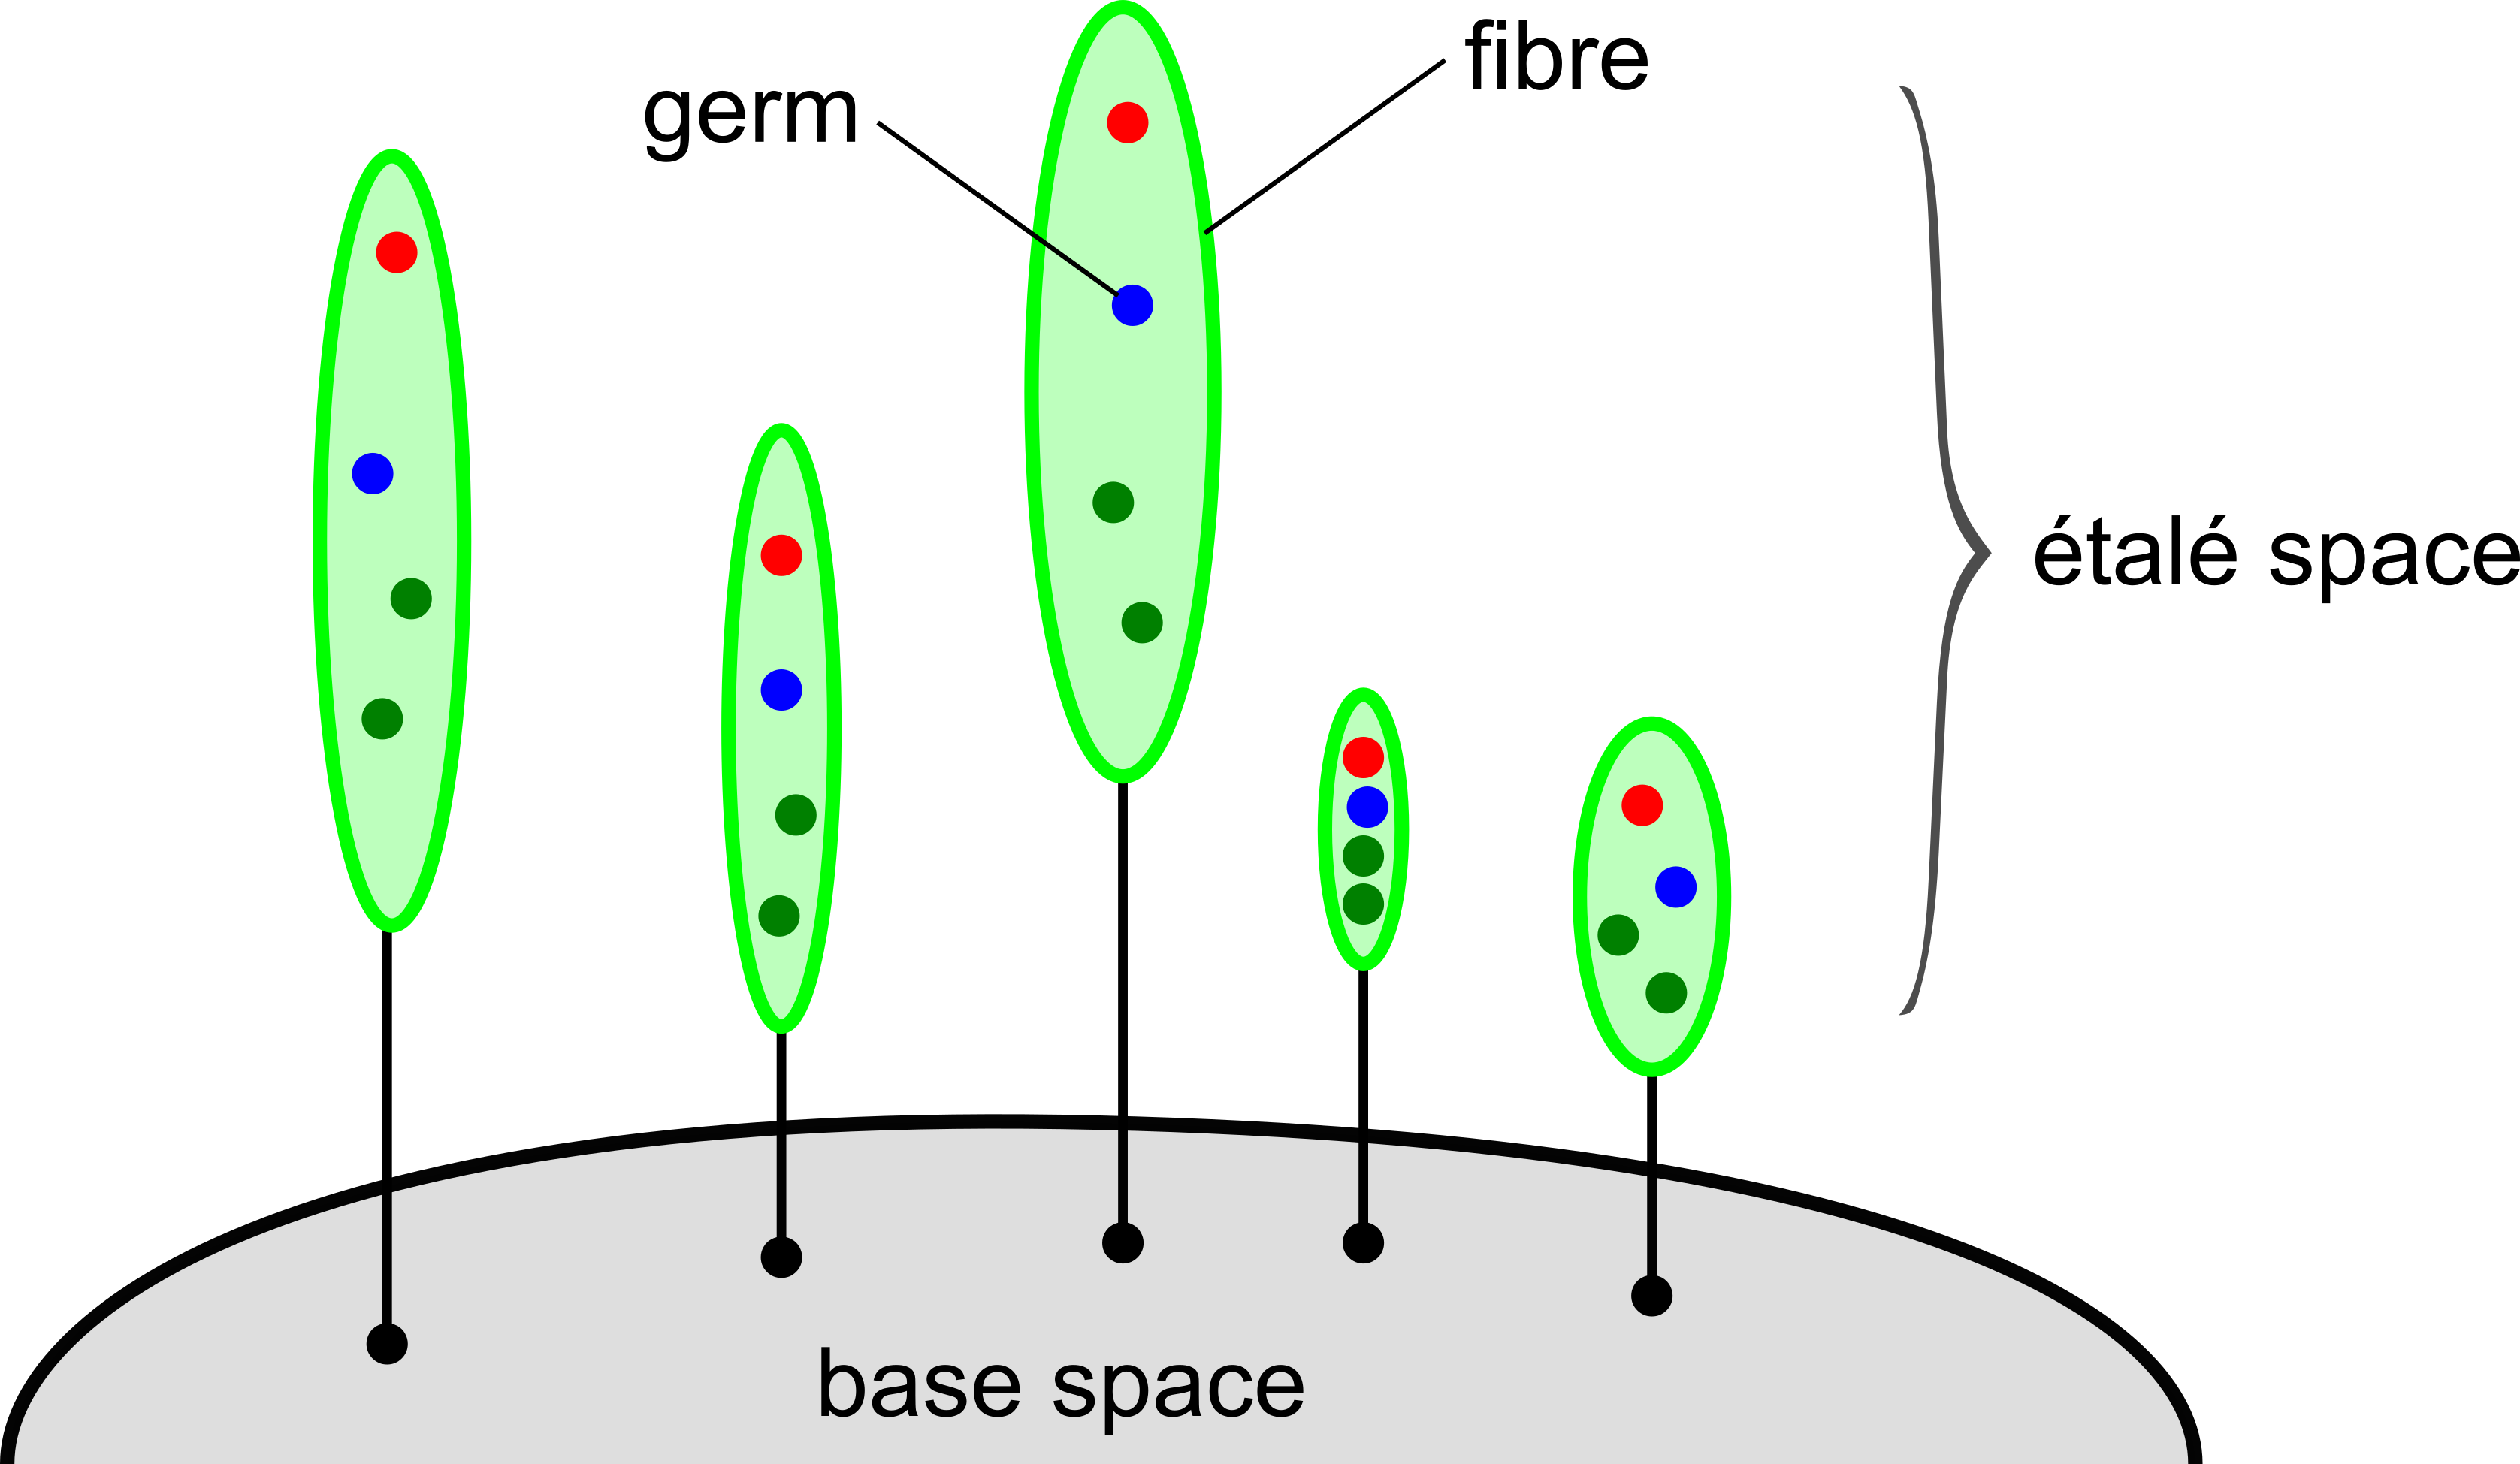
\includegraphics[scale=0.6]{etale-space.png}}}
\end{equation}

\textbf{Propositional logic} is a kind of \textbf{topological} (open set) structure:
\begin{equation}
\vcenter{\hbox{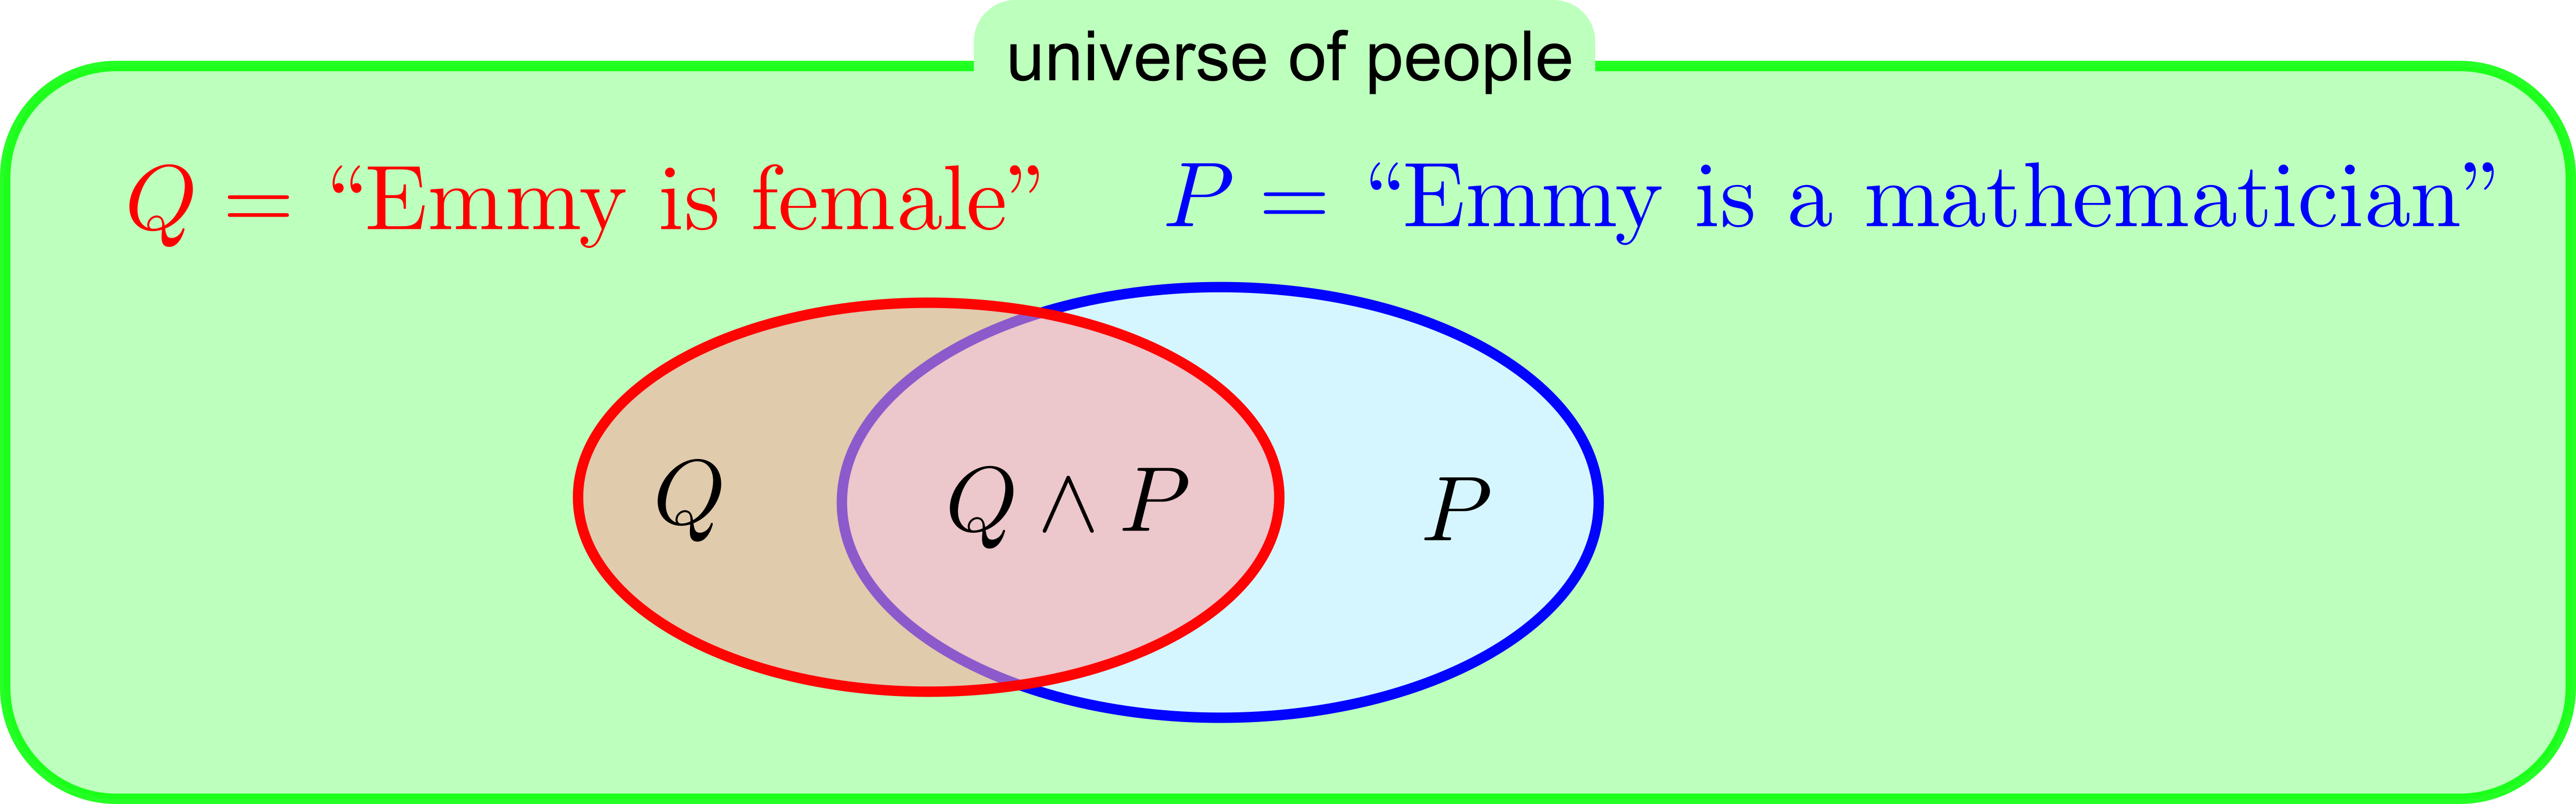
\includegraphics[scale=0.6]{propositional-logic-as-topology.png}}}
\end{equation}

\textit{Inside} a proposition, there is the \textbf{predicate} structure:
\begin{equation}
\vcenter{\hbox{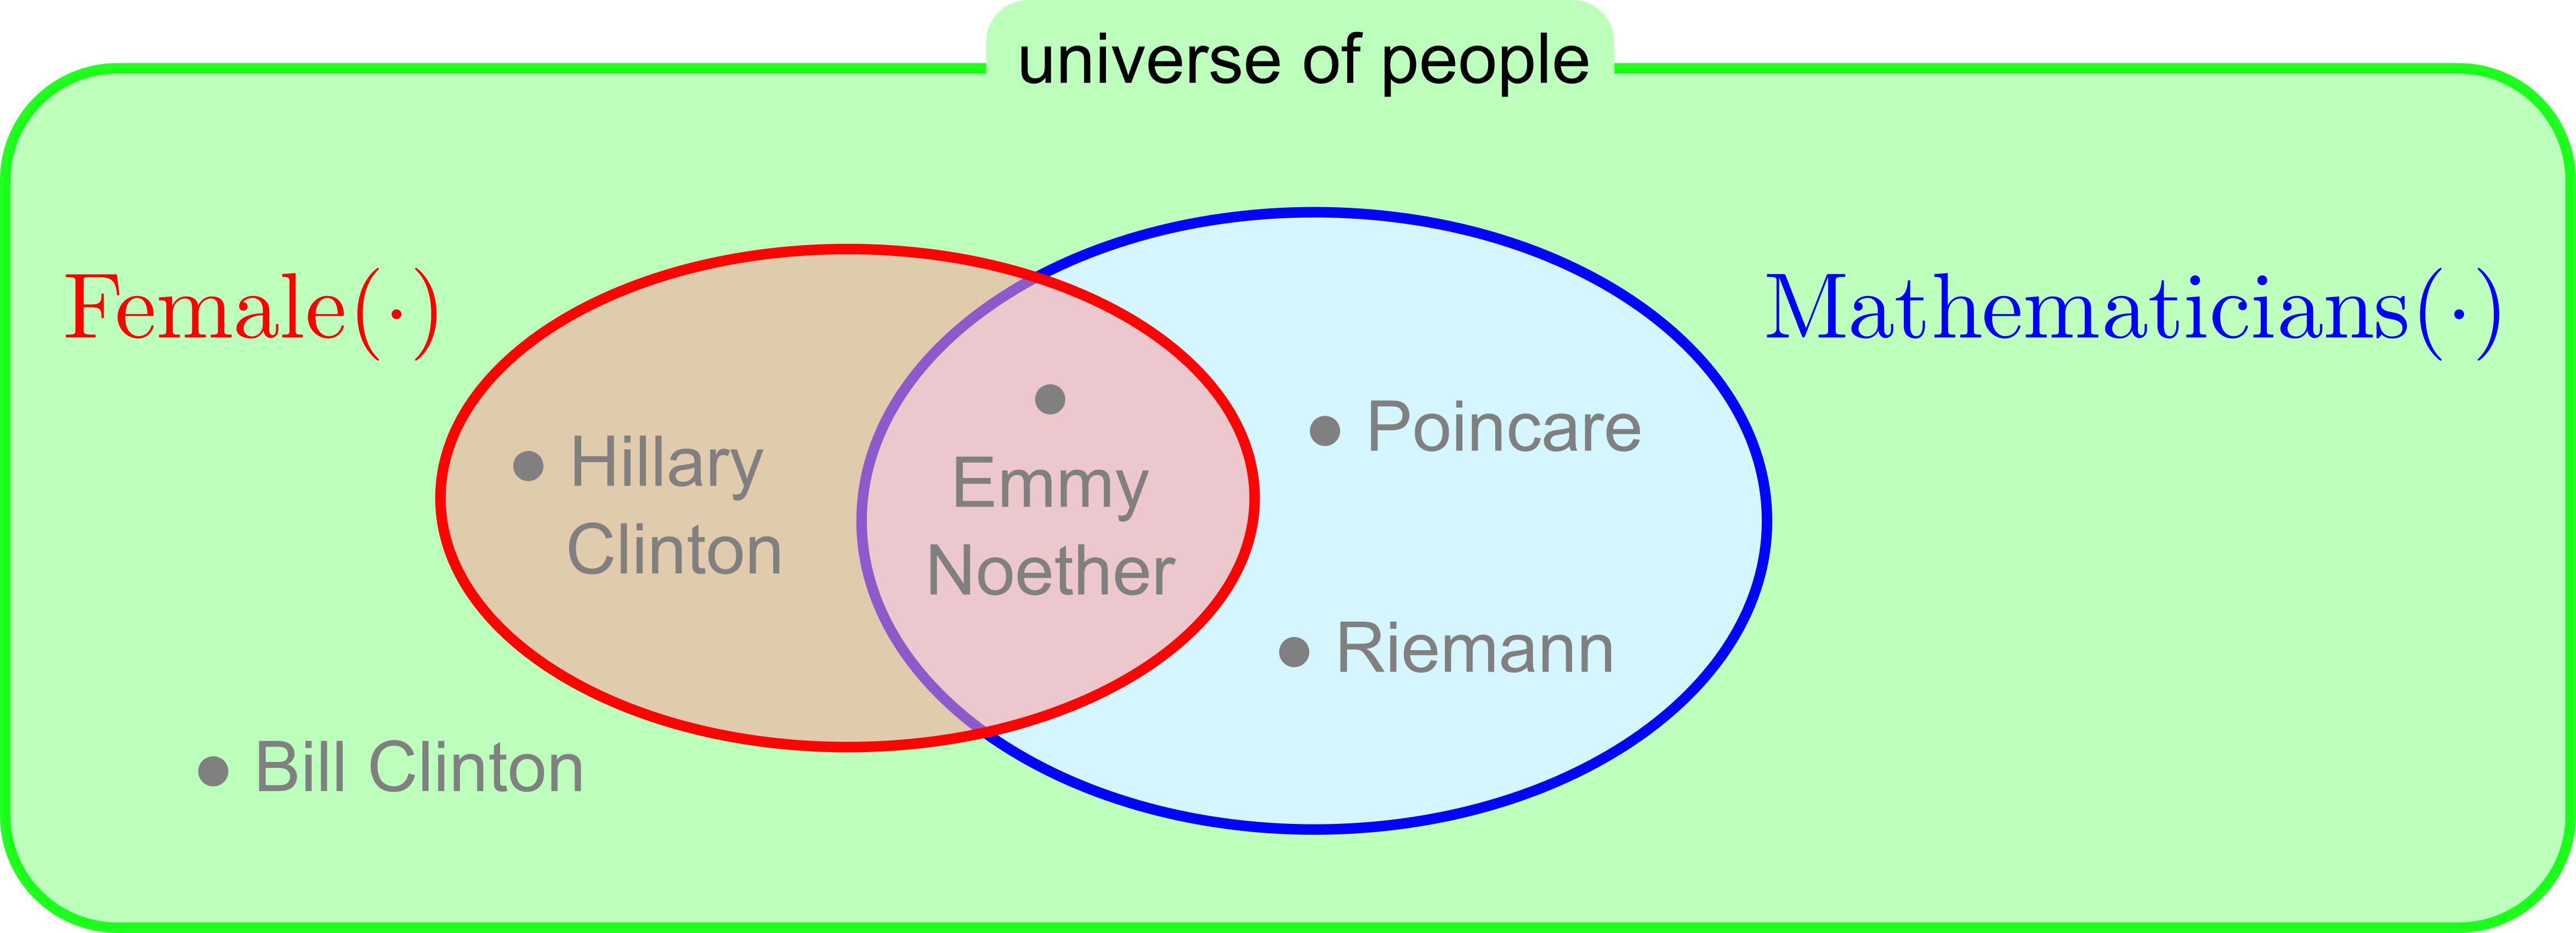
\includegraphics[scale=0.6]{predicate-logic-as-topology.png}}}
\end{equation}

Predicate logic could be regarded as a \textbf{fibration} over propositional structure, denoted as $\mathrel{\substack{\mathbf{Pred}\\\downarrow\\\mathbf{Set}}} $:
\begin{equation}
\vcenter{\hbox{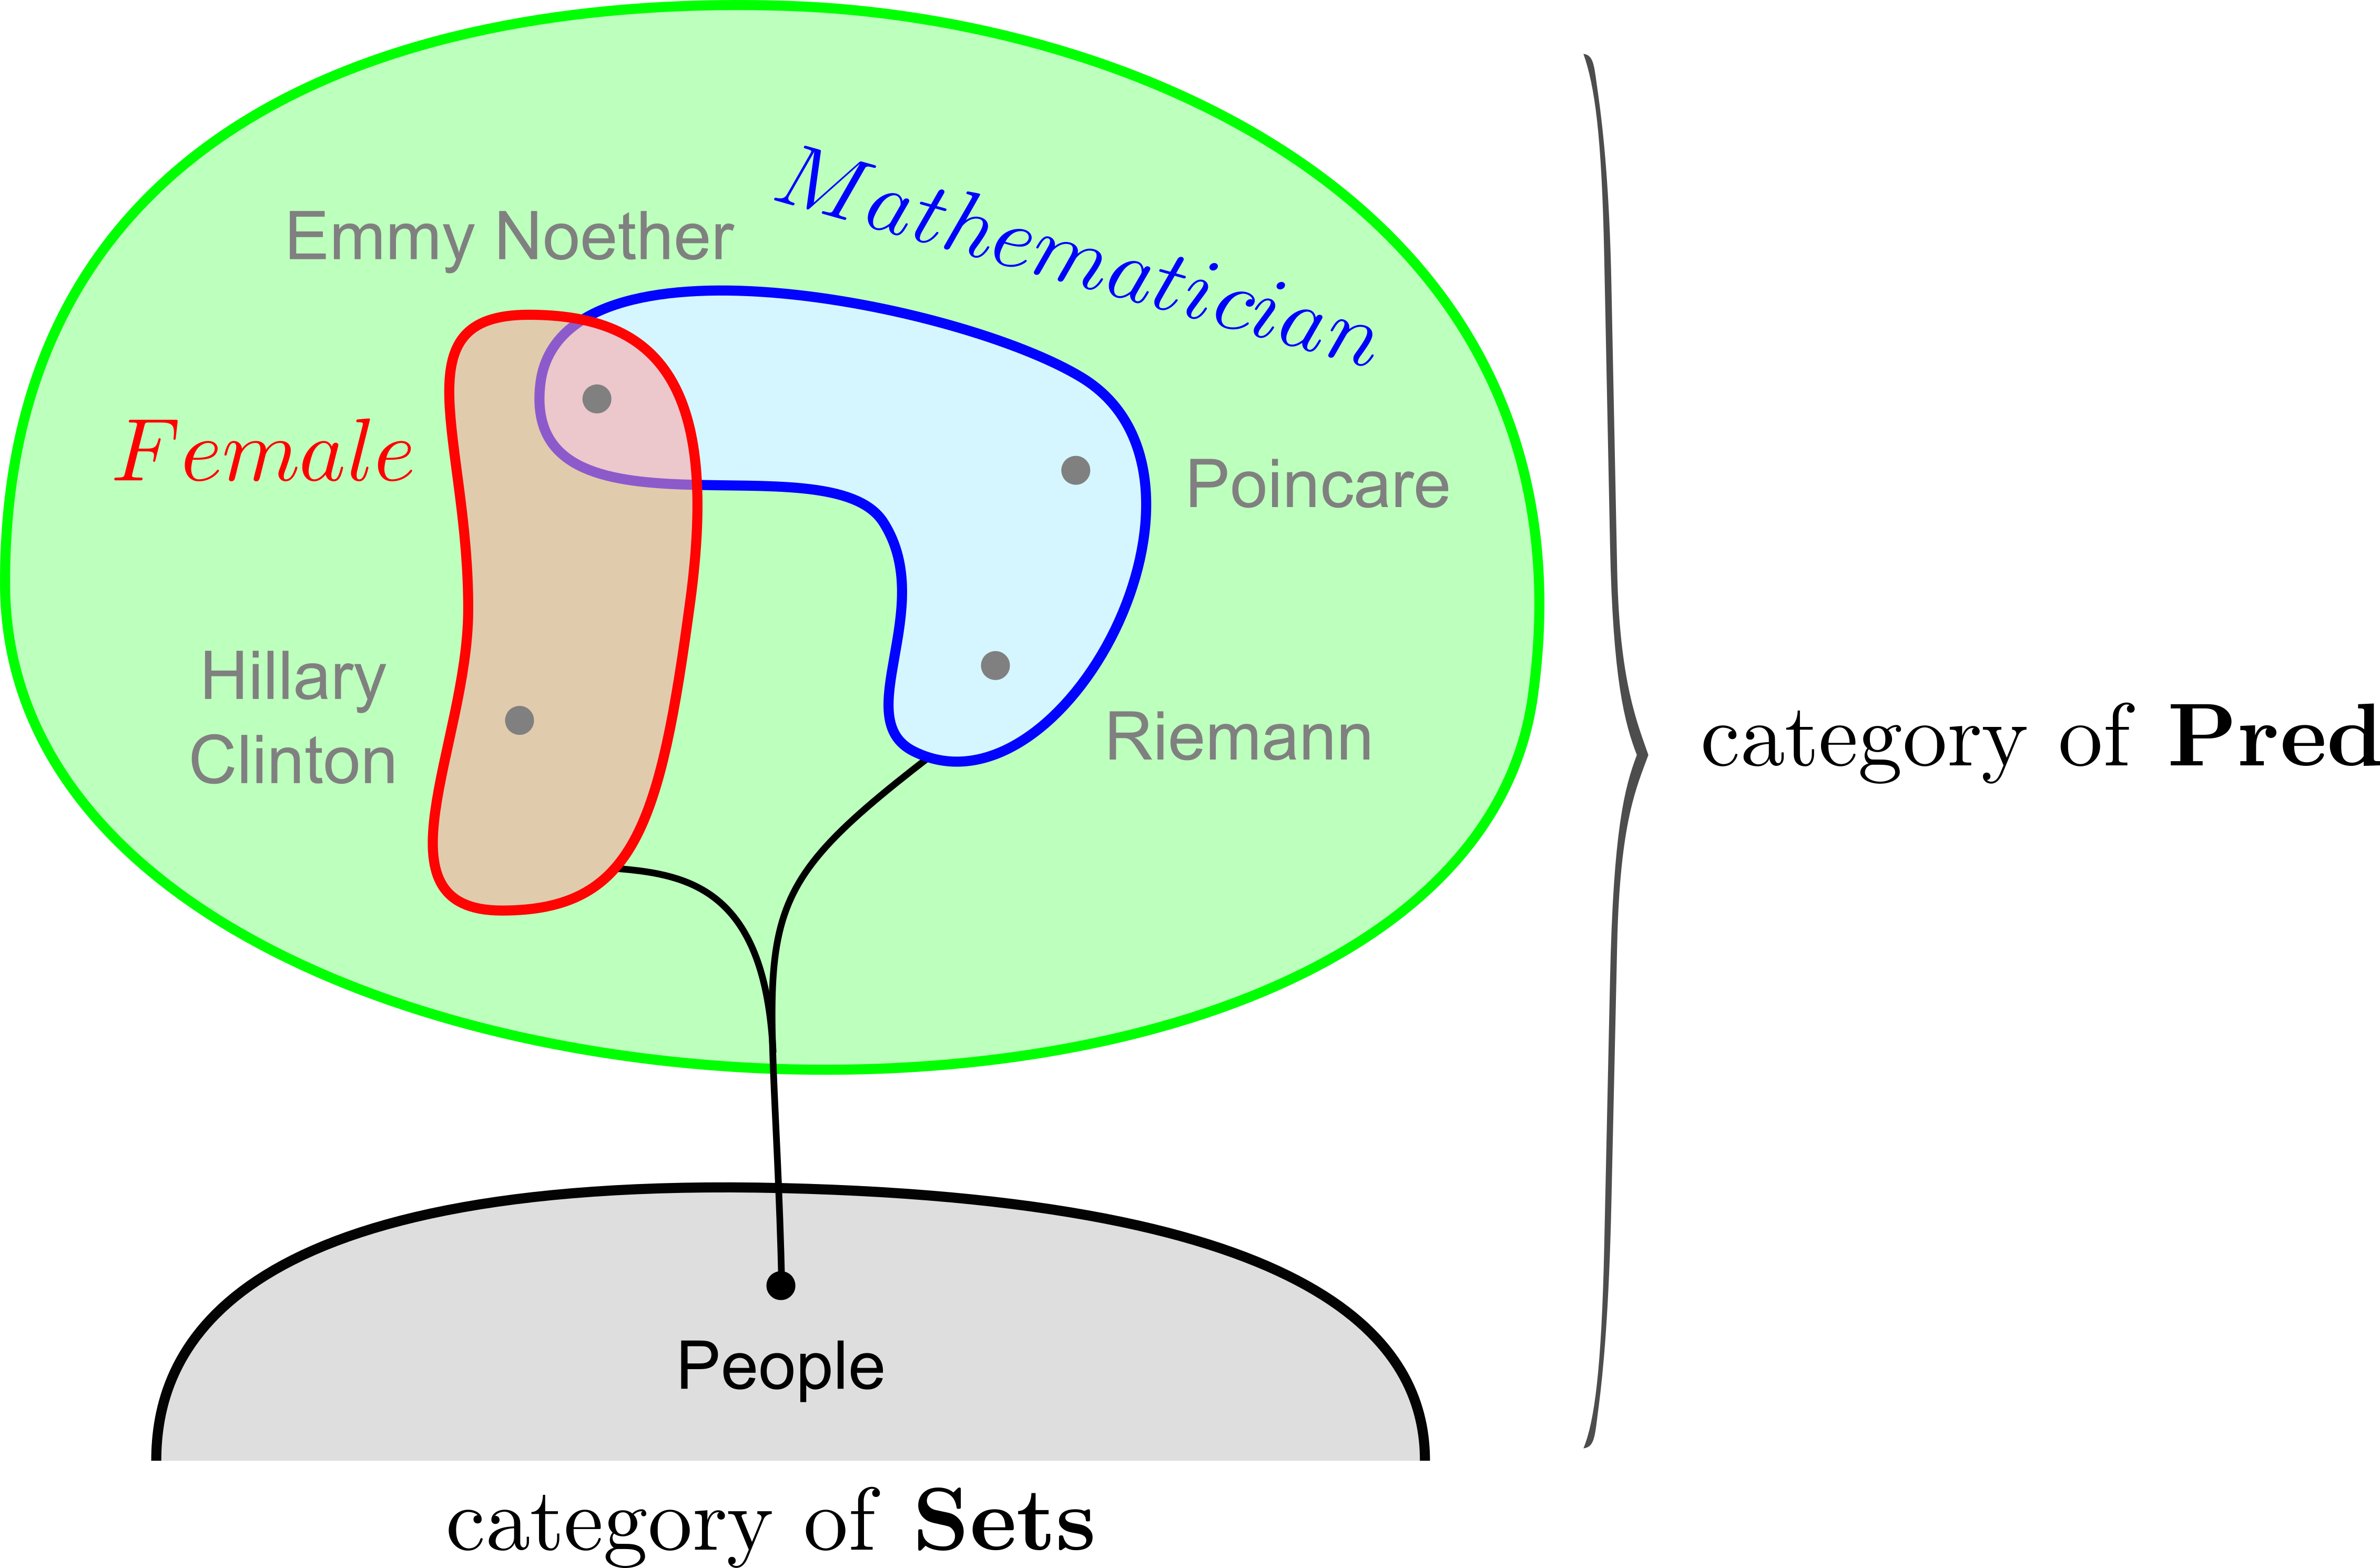
\includegraphics[scale=0.6]{predicate-logic-as-fibration.png}}}
\end{equation}

\subsection{Quantifications are adjoints}

A pair of monotone functions $f: X \rightarrow Y$ and $g: Y \rightarrow X$ between pre-ordered sets determines an \textbf{adjunction}, if $\forall x \in X, y \in Y$:
\begin{equation}
f(x) \le y \mbox{ in } Y \quad \Leftrightarrow \quad x \le g(y) \mbox{ in } X
\end{equation}
in which case we write $f \dashv g$ and say ``$f$ is left-adjoint to $g$'', or ``$g$ is right-adjoint to $f$''.  (Mnemonic: the \textit{left} adjoint appears on the \textit{left} of $\le$ and \textit{vice versa})

Lawvere discovered the following adjunctions:
\begin{equation}
\exists \dashv * \dashv \forall
\end{equation}

In cylindric algebra, the quantifiers $\forall$ and $\exists$ can be interpreted as \textbf{projections} to a component ($X_2$) of the domain:
\begin{equation}
\vcenter{\hbox{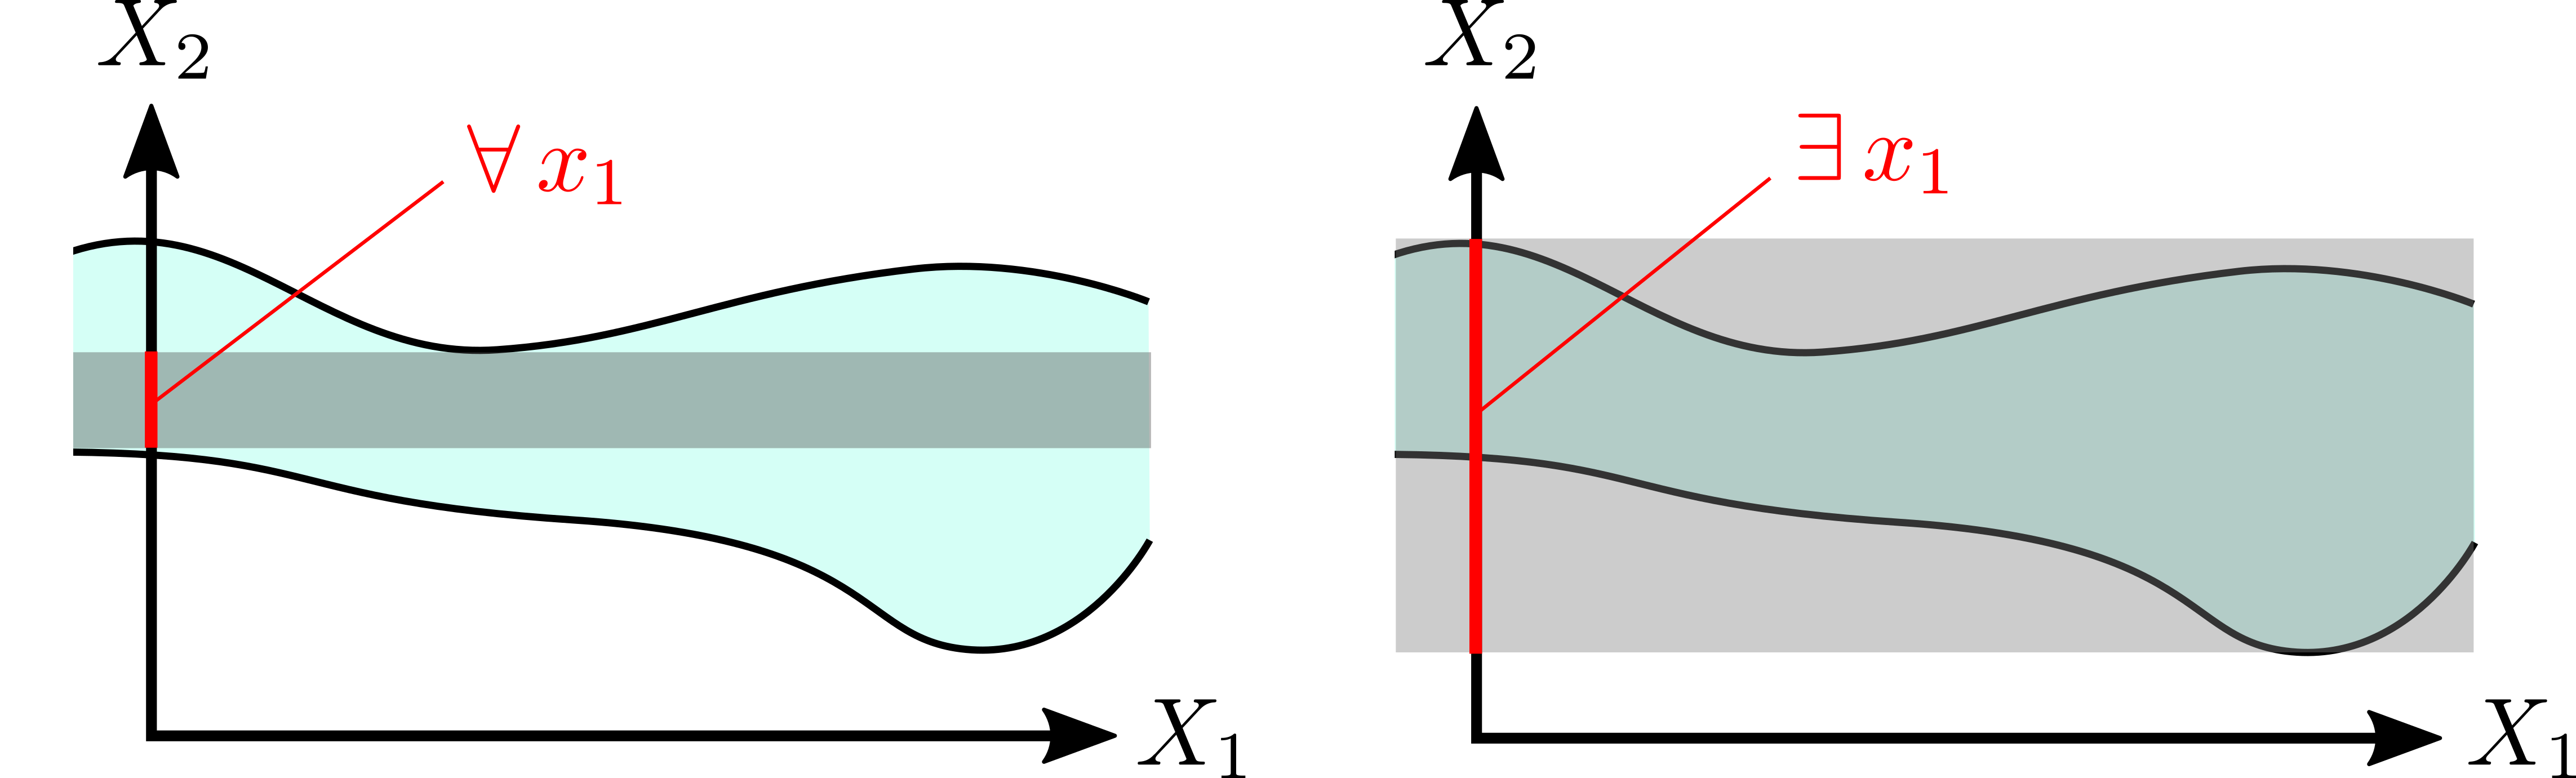
\includegraphics[scale=0.7]{cylindrification-projected.png}}}
\end{equation}

The following 2 formulas are from \parencite{Abramsky2011}.  For all $S \subseteq X, T \subseteq Y$:
\begin{eqnarray}
&S \subseteq f^{-1} T \quad \quad \Longleftrightarrow \quad \quad \exists {}_f  S \subseteq T& \\
&\vcenter{\hbox{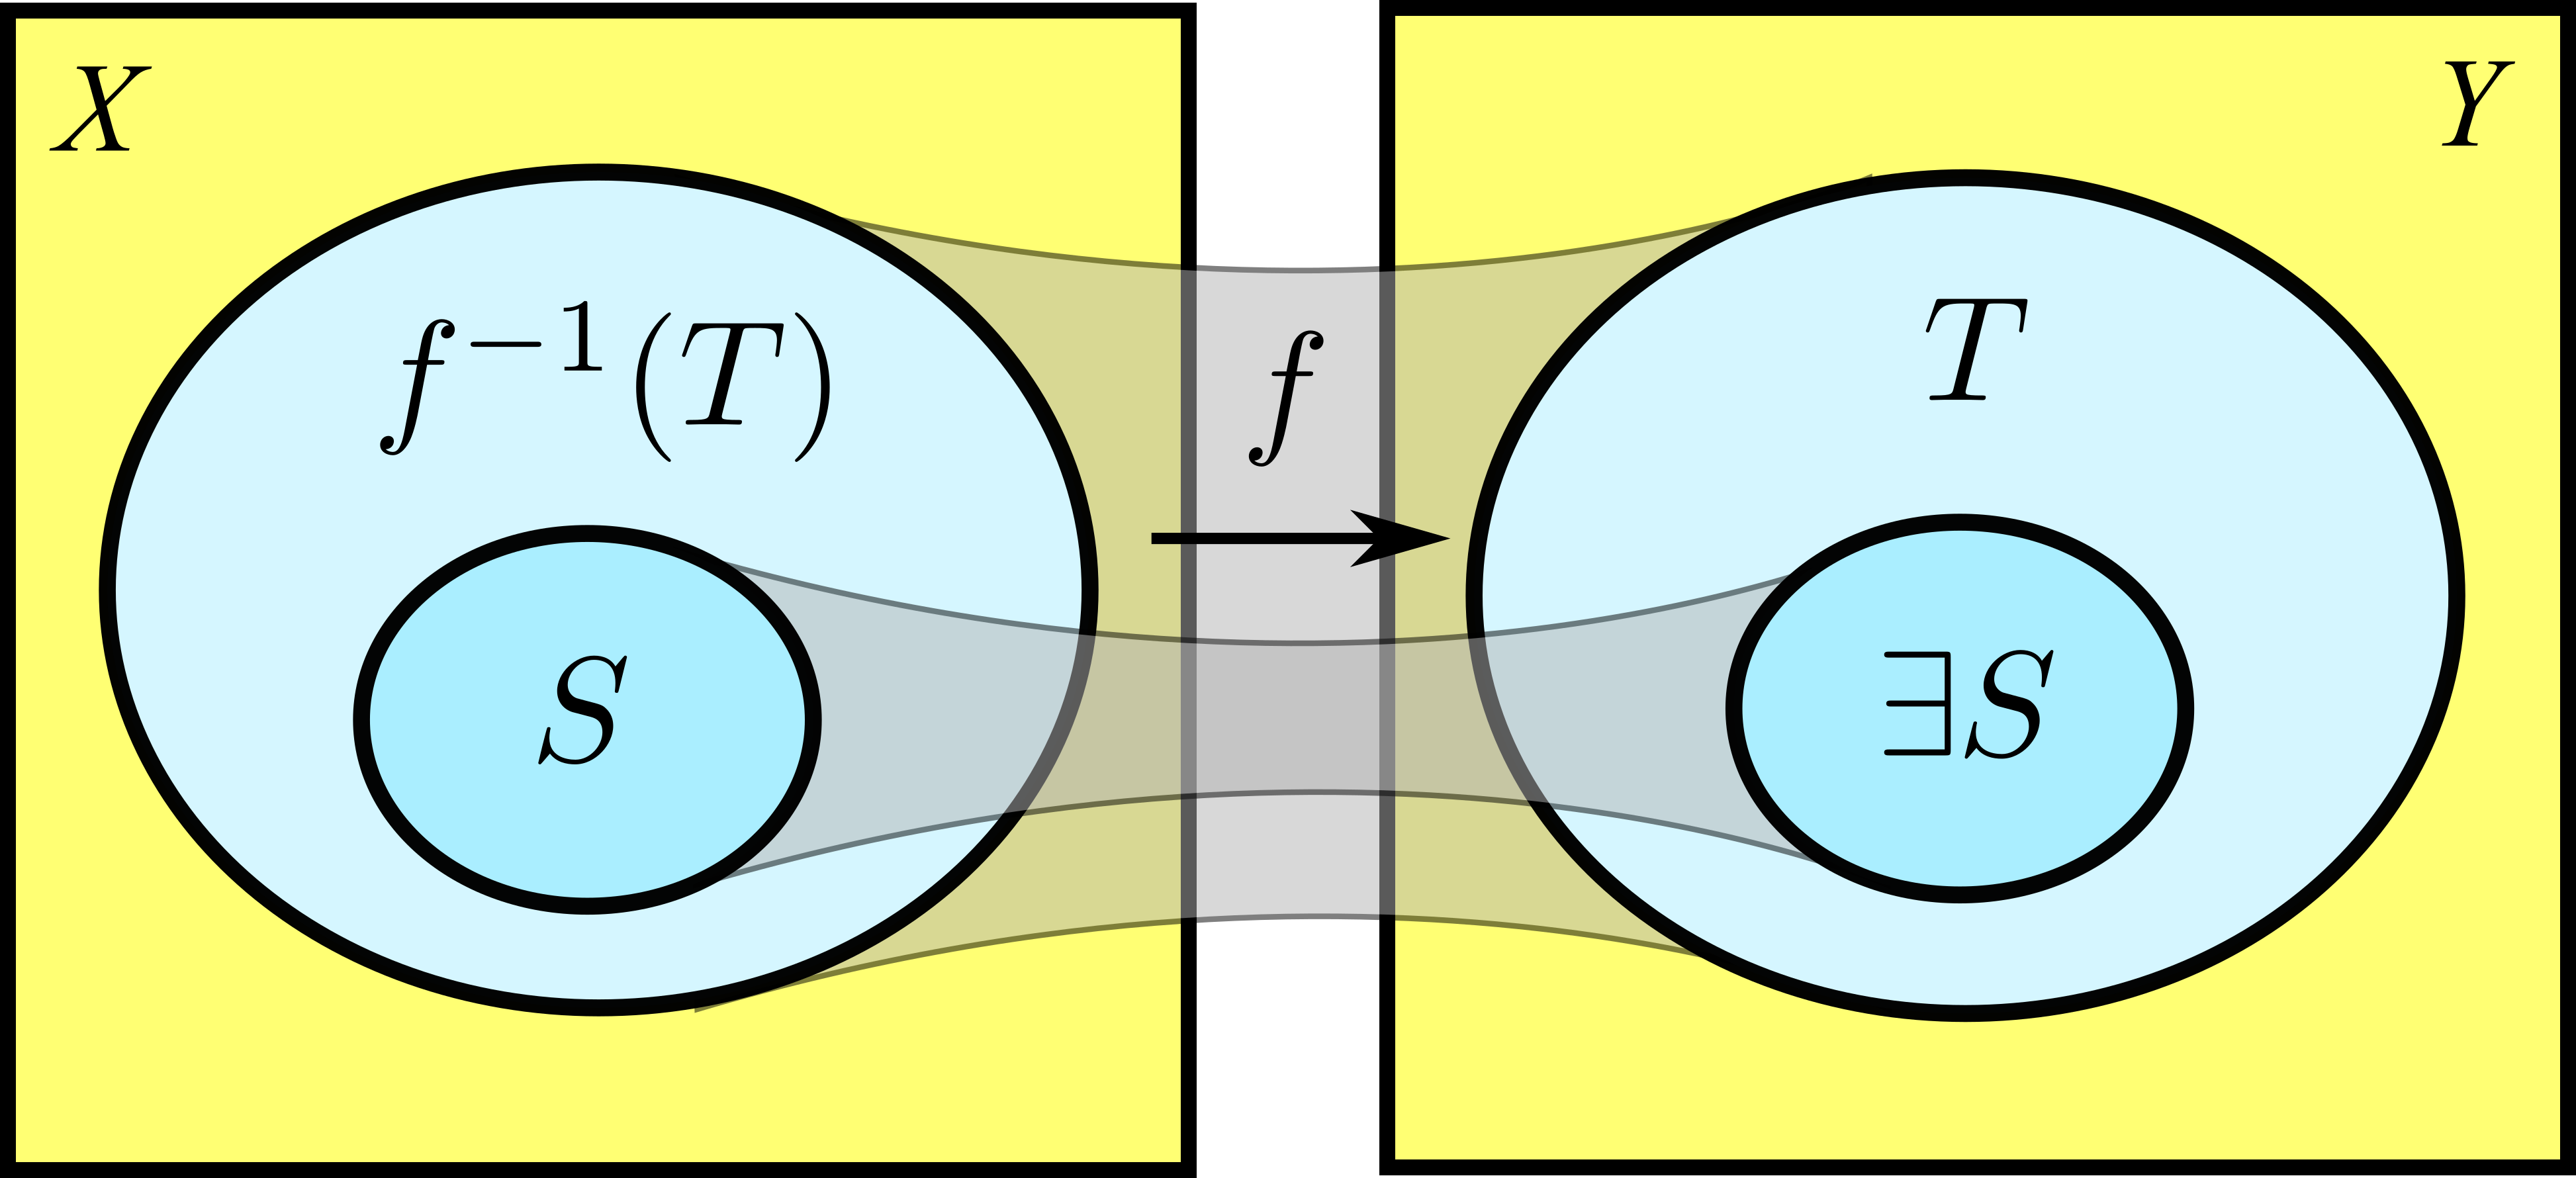
\includegraphics[scale=0.7]{Lawvere-quantifier-exists.png}}}& \nonumber
\end{eqnarray}

\begin{eqnarray}
&f^{-1} T \subseteq S \quad \quad \Longleftrightarrow \quad \quad T \subseteq \forall {}_f  S& \\
&\vcenter{\hbox{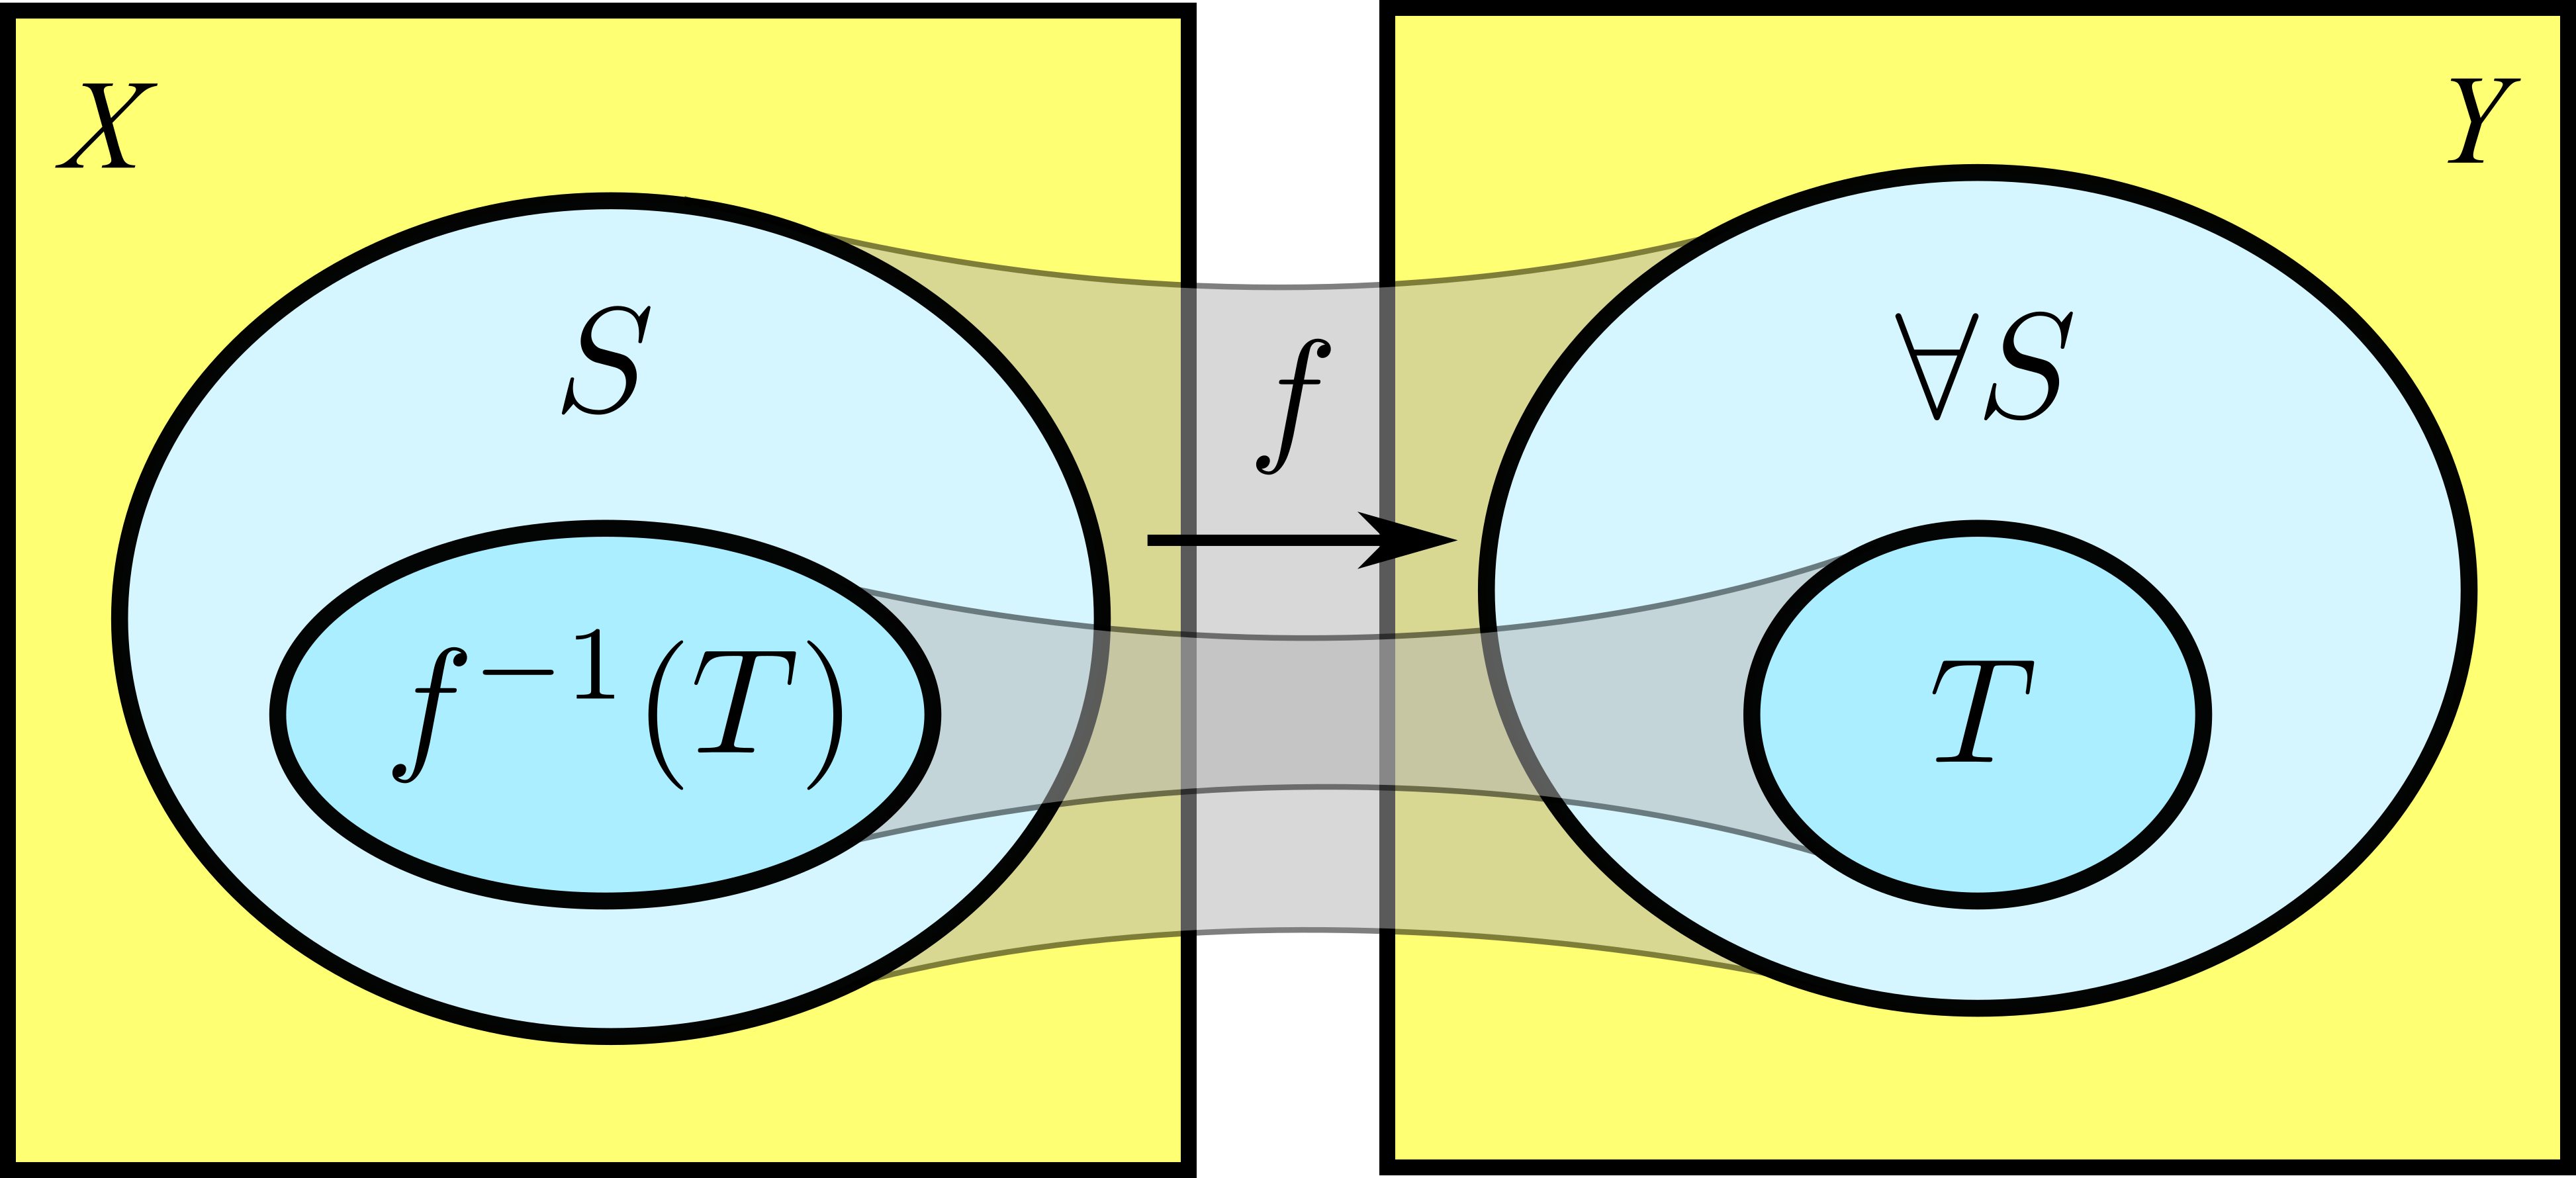
\includegraphics[scale=0.7]{Lawvere-quantifier-forall.png}}}& \nonumber
\end{eqnarray}

They can be interpreted in a ``cylindrical'' way:  Let $X = X_1 \times X_2$ and $Y = X_2$.  Then $f$ is a projection $X_1 \times X_2 \rightarrow X_2$:
\begin{equation}
\vcenter{\hbox{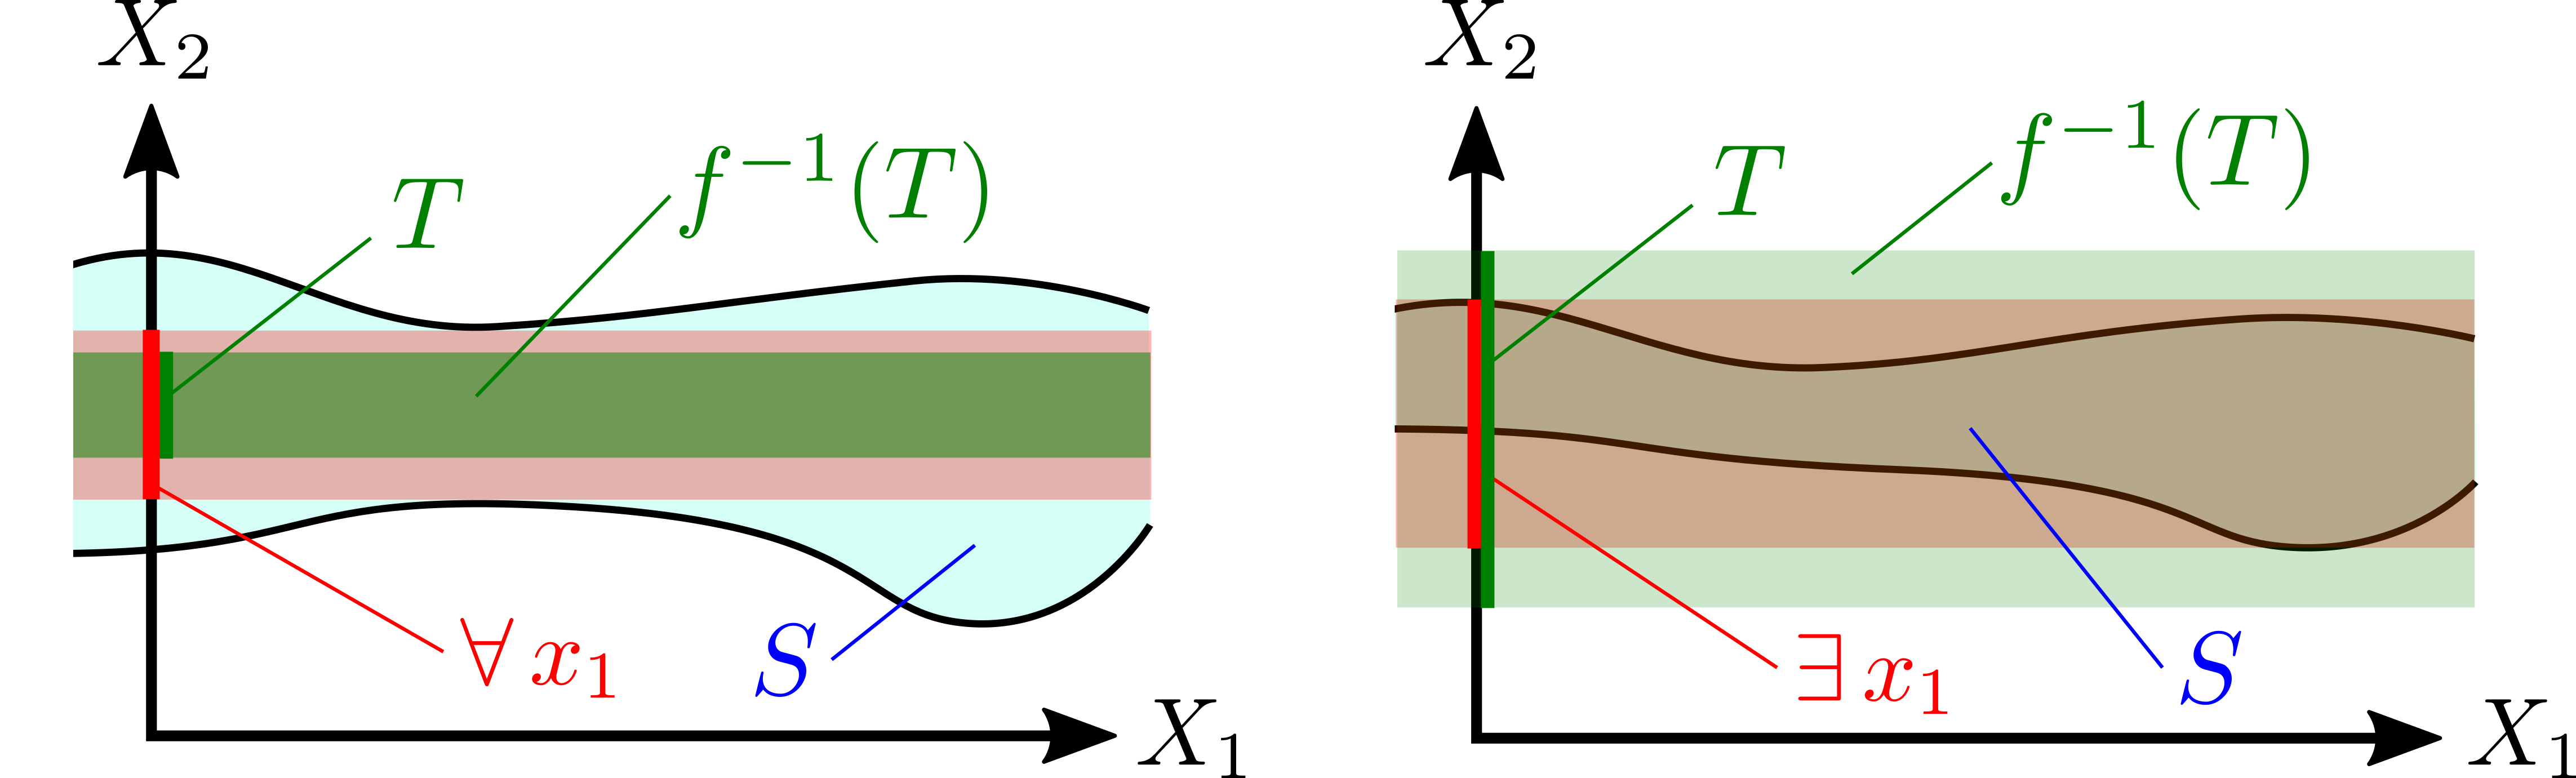
\includegraphics[scale=0.7]{Lawvere-cylindrification.png}}}
\end{equation}

\subsection{Logic in a topos}

In (higher-order) predicate logic we are concerned with sequents of the form:
\begin{equation}
{\color{red} \Gamma \rhd } \; \Phi \vdash \phi
\end{equation}
where $\Phi$ is the \textbf{assumption}, $\phi$ the \textbf{conclusion}, and ${\color{red} \Gamma}$ is a \textbf{variable context} and specifices which free variables are allowed in $\Phi$ and $\phi$.  For example:
\begin{eqnarray}
{\color{red}\mbox{variable context}} & \nonumber \\
{\color{red} \overbrace{ x: \mathbb{N}, y: \mathbb{N} } \;\; \rhd } & \mathrm{odd}(x) \wedge \mathrm{odd}(y) \vdash \mathrm{even}(x + y)
\end{eqnarray}

For every \textbf{type} $\alpha$ in the signiture we have an object $\llbracket \alpha \rrbracket$ of $\mathscr{C}$.

For every \textbf{proved term} $\Gamma \vdash M : \alpha$, we have a morphism in $\mathscr{C}$:
\begin{equation}
\llbracket \Gamma \vdash M : \alpha \rrbracket : \llbracket \Gamma \rrbracket \rightarrow \llbracket \alpha \rrbracket
\end{equation}

For $A \in \mathrm{Obj} \; \mathscr{C}$, the set of \textbf{predicates} in $A$ = $\mathrm{Sub}_{\mathscr{C}}(A) \cong \mathscr{C}(A, \Omega)$, with a partial order $\le_A$ on it.

\subsection{Categorical semantics}

\cc{Categorical semantics 是用 category theory 表达的 model theory。
}{
Categorical semantics is model theory expressed in category theory.}

We have the following duality:
\begin{itemize}
\item Every algebraic / logic theory $Th$ has a \textbf{classifying category} $Cl(Th)$
\item Every category $\mathscr{C}$ with finite products has an \textbf{internal language} $Th(\mathscr{C})$
\end{itemize}
with the equivalences:
\begin{eqnarray}
& Cl(Th(\mathscr{C})) \simeq \mathscr{C} \nonumber \\
\mbox{and } & Th \simeq Th(Cl(Th))
\end{eqnarray}

According to nLab:  The \textbf{Mitchell–B\'{e}nabou language} is a particularly simple form of the internal language of an elementary topos $\mathscr{E}$.  In \parencite{Streicher2006} it is show that an arbitrary elementary topos $\mathscr{E}$ can interpret \textbf{higher-order intuitionistic (constructive) logic}.

The category $Cl(Th)$ has:
\begin{itemize}
\item objects = finite lists of types, \textit{eg}, $\vec{\alpha} = [\alpha_1, ..., \alpha_n] $
\item morphisms from source $\vec{\alpha}$ to target $\vec{\beta}$ = $[(\Gamma|M_1), ..., (\Gamma|M_m)] : \vec{\alpha} \rightarrow \vec{\beta}$
\end{itemize}
where $(\Gamma|M)$ is an equivalence class of pairs $(\Gamma, M)$ of contexts and raw terms:

We define a \textbf{category of models} $\mathbf{Mod}(Th, \mathscr{C})$:
\begin{itemize}
\item objects = models of $Th$ in $\mathscr{C}$
\item morphisms = homomorphisms of models of $Th$ in $\mathscr{C}$
\end{itemize}
and we define another category $\mathbf{FP}$ (for finite product) that has:
\begin{itemize}
\item objects = finite-product preserving functors
\item morphisms = natural transformations
\end{itemize}
then we can define a \textbf{modelling functor} $Ap_G$:
\begin{equation}
Ap_G: \; \mathbf{FP}(Cl(Th), \mathscr{D}) \rightarrow \mathbf{Mod}(Th, \mathscr{D})
\end{equation}

\book{以下内容主要来自 \parencite{Caramello2018} 这本新书的第一章。  更经典的参考书是 \parencite{Goldblatt1984}.  范畴论最好的入门书当然是「中学生也能看懂的」\textit{Conceptual mathematics} \parencite{Lawvere1997} 还有 \parencite{Lawvere2003}.}

\cc{不同的 logics 可以透过 \textbf{proof theory}(它研究的是 \textit{syntactic} rules of deduction)定义:
}{
Different logics can be defined by \textbf{proof theory} (which studies \textit{syntactic} rules of deduction):}
\begin{equation}
\begin{tabular}{|l|l|}
\hline
algebraic logic & no additional rules\\
\hline
Horn logic & finite $\wedge$ \\
\hline
regular logic & finite $\wedge$, $\exists$, Frobenius axiom\\
\hline
coherent logic & finite $\wedge$ and $\vee$, $\exists$,\\
				& distributive axiom, \\
				& Frobenius axiom \\
\hline
geometric logic & finite $\wedge$, infinitary $\vee$, $\exists$,\\
				& infinitary distribution axiom,\\
				& Frobenius axiom \\
\hline
first-order intuitionistic logic & all finitary rules \\
				& except law of excluded middle\\
\hline
first-order classical logic & all finitary rules \\
\hline
\end{tabular}
\end{equation}

\cc{举例来说,\textbf{algebraic theory} 的意思是: 它只有一个 relation $=$,而所有 axioms 都是 $s = t$ 这种形式。 
}{
For example, \textbf{algebraic theory} means: It has only one relation $=$, and all axioms are of the form $s = t$.}

\cc{还有这些 deduction rules 的例子:
}{
There are also examples of these deduction rules:}
\begin{equation}
\boxed{\wedge \mbox{ rule}}	\quad \frac{\Phi \vdash \Psi, \; \Phi \vdash \Chi}{\Phi \vdash (\Psi \wedge \Chi)}
\end{equation}
\vspace*{-5pt}
\begin{equation}
\boxed{\exists \mbox{ double rule}}	\quad \Dfrac{\Phi \vdash_{\vec{x}, y} \Psi}{\exists y \, \Phi \vdash_{\vec{x}} \Psi}
\end{equation}
\begin{equation}
\boxed{\mbox{Frobenius axiom}}	\quad \Phi \wedge \exists y \, \Psi \vdash_{\vec{x}} \exists y \, (\Phi \wedge \Psi)
\end{equation}

\cc{Tarski 的模型论 将 first-order syntax 「对应」到 集合论 的 \textbf{结构} (structures) 上。  由此推广,不同的 逻辑 syntax 对应於不同的 结构范畴:
}{
Tarski's model theory "corresponds" the first-order syntax to the \textbf{structure} of the set theory. As a result, different logical syntaxes correspond to different structural categories:}
\begin{equation}
\begin{tabular}{|l|l|}
\hline
categories with finite products & algebraic logic \\
\hline
Cartesian categories			& Cartesian logic \\
\hline
regular categories				& regular logic \\
\hline
coherent categories				& coherent logic \\
\hline
geometric categories			& geometric logic \\
\hline
Heyting categories				& first-order intuitionistic logic \\
\hline
Boolean coherent categories		& first-order classical logic \\
\hline
\end{tabular}
\end{equation}

The term ``Geometric'' logic comes from \textbf{geometric morphisms}, which is a kind of morphism between 2 toposes that are particularly ``natural'' to define, similar to \textbf{continuous maps} between topological spaces.

A \textbf{geometric morphism} between 2 elementary toposes, $f: \mathscr{C}_1 \rightarrow \mathscr{C}_2$ , is a pair of functors of the form:
\begin{equation}
\begin{tikzcd}[column sep = large]
\mathscr{C}_1 \arrow[r, shift right, swap, "f_*"] 
& \mathscr{C}_2 \arrow[l, shift right, swap, "f^*"]
\end{tikzcd}
\end{equation}
such that $f^*$ is \textbf{left exact} and left adjoint to $f_*$.

A functor is called \textbf{left exact} if it preserves all finite limits (\textit{ie}, limits of all finite diagrams).  Dually, a \textbf{right exact} functor preserves all finite co-limits.

\cc{以下是根据 \parencite{Caramello2018} Ch.1 整理出来的一张关系图: 
}{
I made the following diagram from \parencite{Caramello2018} Ch.1:}
\begin{equation}
\vcenter{\hbox{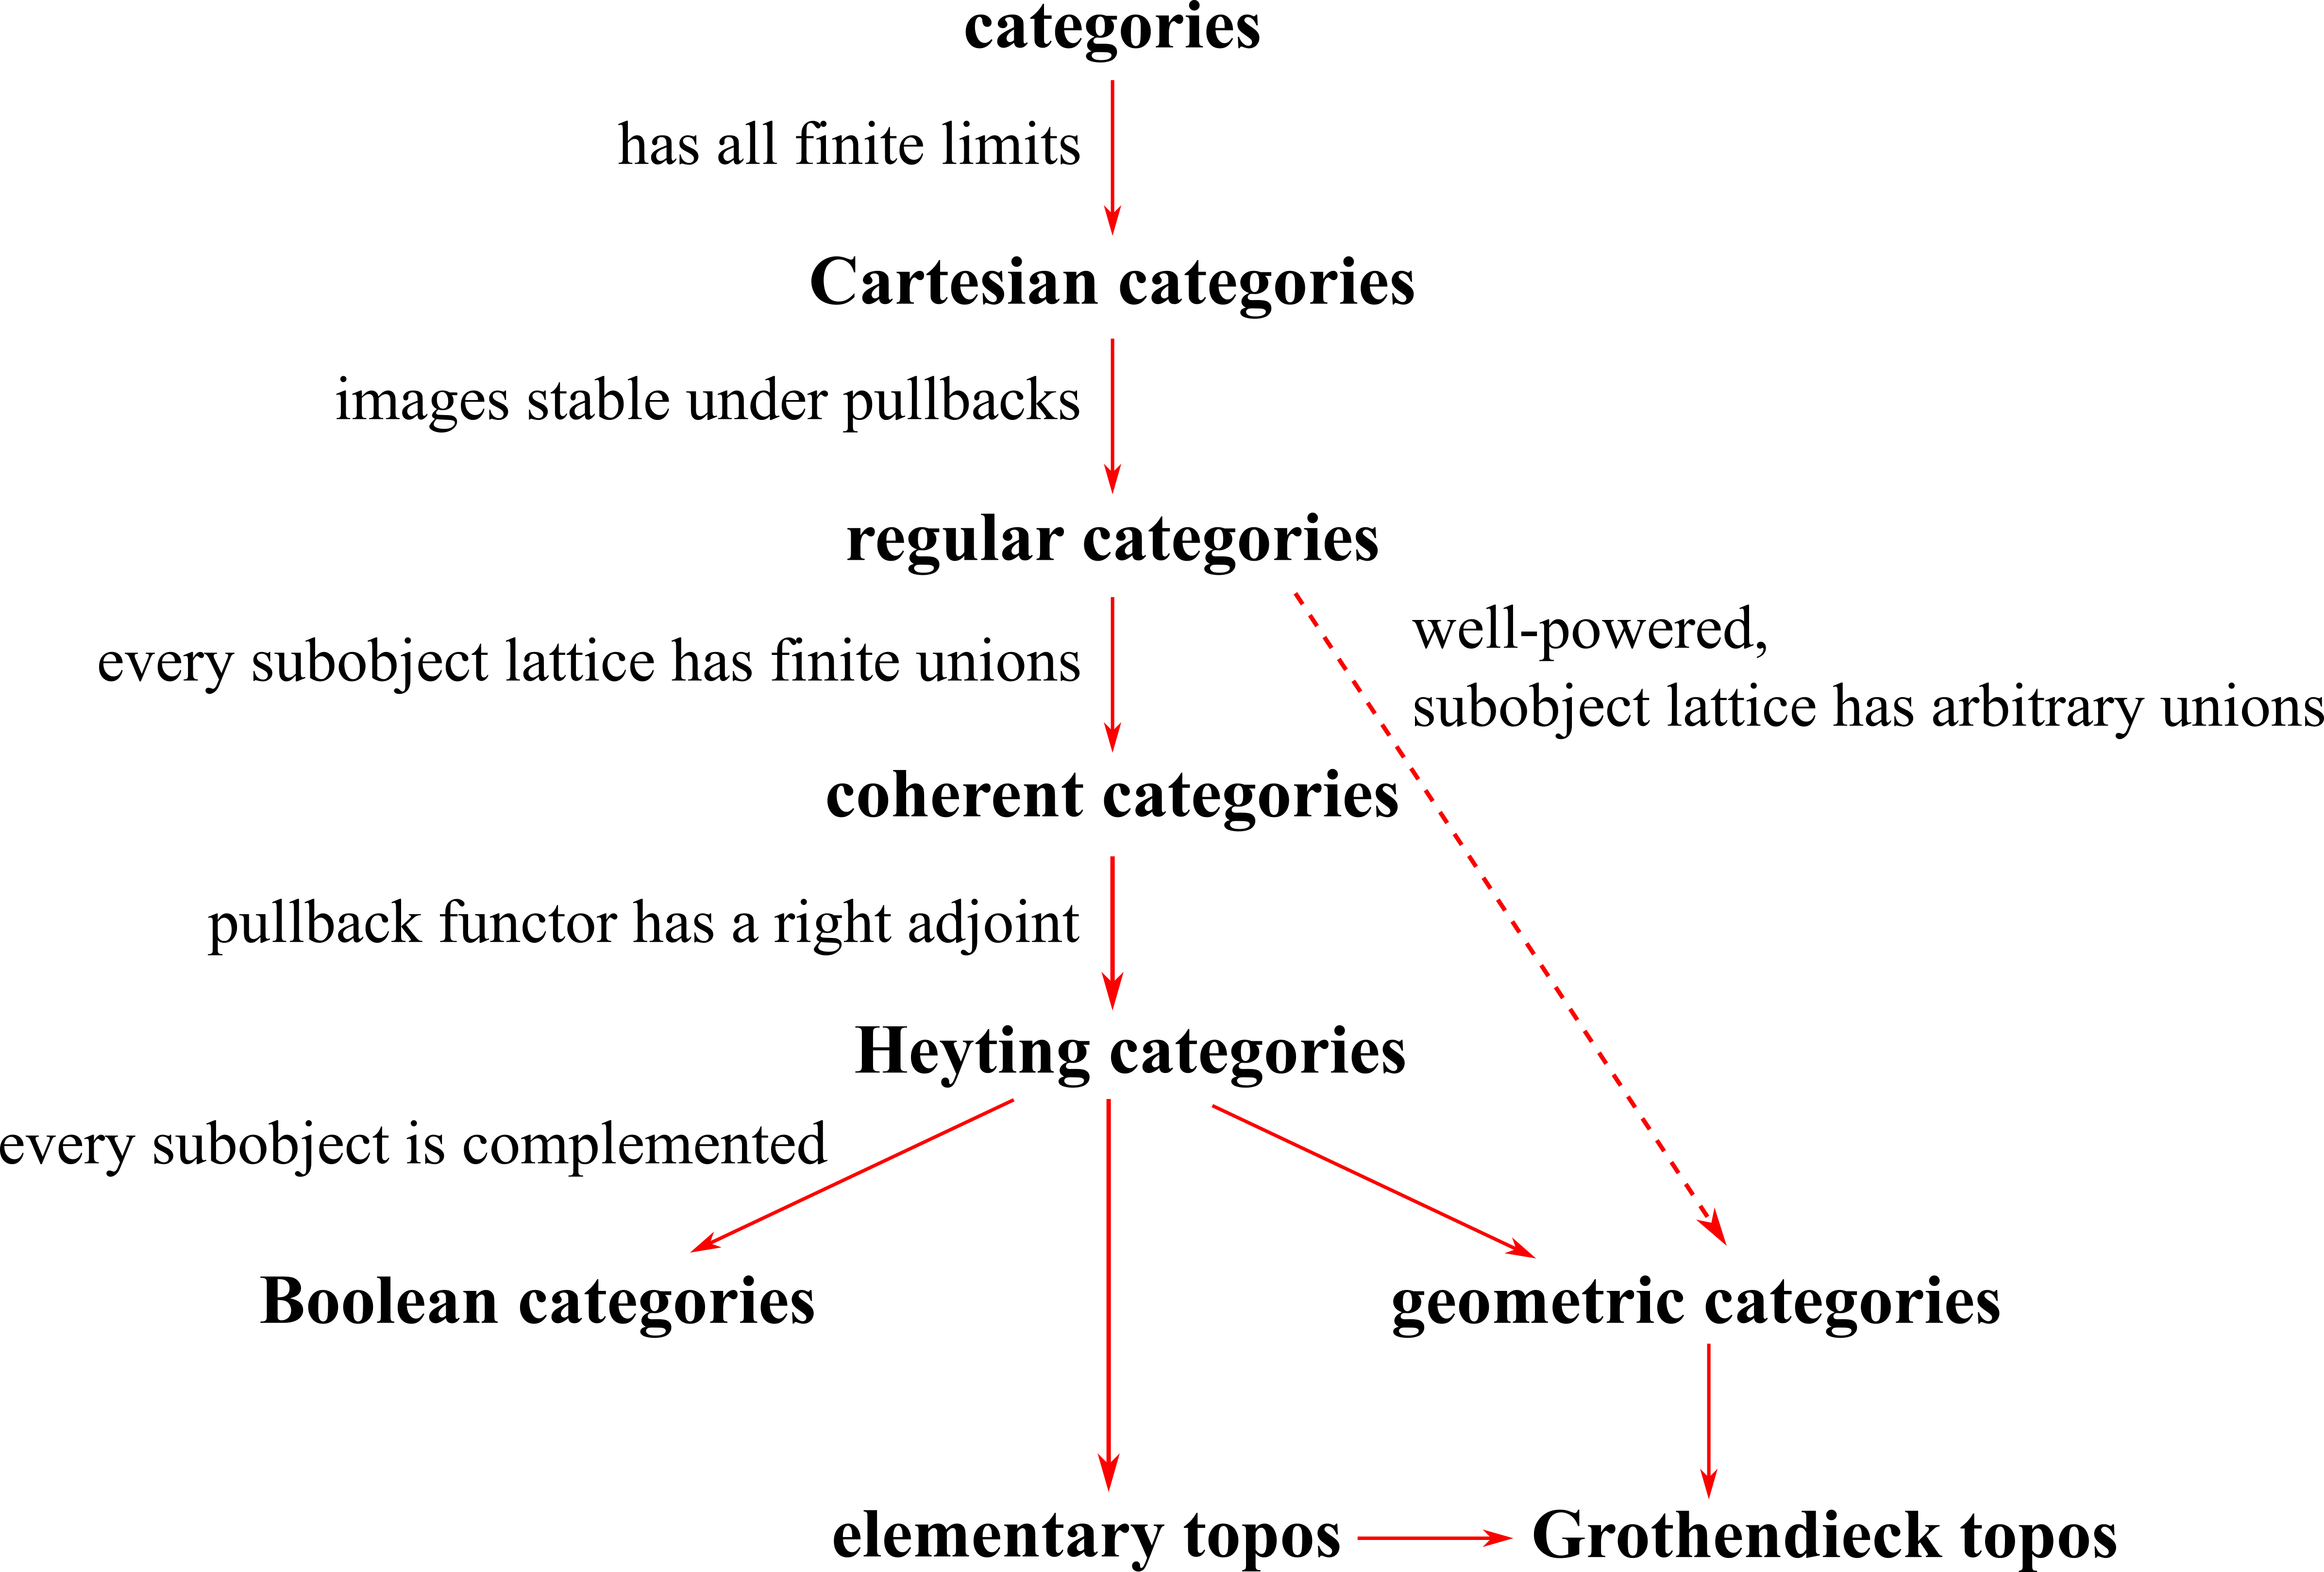
\includegraphics[scale=0.7]{logical-categories.png}}}
\end{equation}

Grothendieck's idea of topos is a \textit{stronger} notion than elementary topos.

\subsection{Fuzzy logic}

\book{ From \S 5.2.4 of \parencite{Klir2017}. }

In any topos one may define arrows which play the role of \textbf{truth functions} of logical connectives on $\Omega$.  In this sense, each topos ``internalizes'' a logic.  It is a striking fact that, in general, $\Omega$ becomes a Heyting algebra and thus the internal logic of topoi is intuitionistic logic.

An early attempt of a category of fuzzy sets is $\mathbf{S}(L)$ proposed by Goguen.  For a complete residuated lattice $L$, $\mathbf{S}(L)$ has as \textbf{objects} the pairs $\langle U, A \rangle$ where $U$ is a set and $A$ an $L$-set of $U$, \textit{ie}, $A: U \rightarrow L$, \textit{ie}, a subset of $U$ fuzzified by $L$; and as \textbf{morphisms} $R: \langle U, A \rangle \rightarrow \langle V, B \rangle$ the $L$-relations $R: U \times V \rightarrow L$ satisfying $\bigvee_{u \in U} \; A(u) \otimes R(u,v) \le B(v) $, along with $\circ$-composition.  This is later shown to be a \textbf{quasi-topos}.

In 1981 Eytan described a category of \textbf{Heyting-algebra-valued sets}, similar to Goguen's $\mathbf{S}(L)$, and claimed that it forms a topos, which was disproved by Pitts the next year.


\subsection{Graphs}

The category of graphs is a functor category:
\begin{equation}
\mathbf{Graphs} = \mathbf{Sets}^\Gamma
\end{equation}
where $\Gamma$ is a category pictured as follows:
\begin{equation}
\begin{tikzcd}[column sep = large]
\bullet \arrow[r, shift left] \arrow[r, shift right] & \bullet
\end{tikzcd}
\end{equation}
It has exactly 2 objects and 2 distinct arrows.  It follows from this that $\mathbf{Graphs}$ is Cartesian-closed \parencite{Awodey2006} p.143.

\subsection{Homotopy type theory}

\book{ \parencite{Rodin2014} }

2 continuous maps:
\begin{equation}
\begin{tikzcd}[column sep = large]
A \arrow[r, shift left, "f"] \arrow[r, shift right, swap, "g"] & B
\end{tikzcd}
\end{equation}
between 2 spaces $A, B$ from $\mathbf{Top}$ are called \textbf{homotopical} when there exists a homotopy between them.  A homotopy $h$ between 2 continuous maps $f,g: A \rightarrow B$ in $\mathbf{Top}$ is a continuous map $h: A \times [0,1] \rightarrow B$ such that $h(0) = f$ and $h(1) = g$.

By identifying all homotopic maps in $\mathbf{Top}$ one gets the \textbf{homotopy category} $\mathbf{hTop}$.

Quillen in 1967 axiomatized homotopy theory as the \textbf{model category}.  Awodey and Warren showed that every model category admits an internal language, which is a form of Martin-L\"{o}f type theory.

Voevodsky provided this inductive definition:
\begin{enumerate}
\item A space $A$ is called \textbf{contractible} (a.k.a. a space of $h$-level 0) when there is a point $x: A$ connected by a path with each point $y: A$ in such a way that all these paths are homotopic.

\item We say that $A$ is a space of $h$-level $n + 1$ if for all points $x, y$ the path spaces $\mathrm{Path}_A (x,y)$ are of $h$-level $n$.
\end{enumerate}

Then we have these hierarchical levels:

\begin{itemize}
\item \textbf{Level 0:} up to homotopy equivalence there is just one contractible space that we call ``point'' and denote $pt$

\item \textbf{Level 1:} up to homotopy equivalence there are 2 spaces at this level:  the \textbf{empty space} $\varnothing$ and the \textbf{point} $pt$.  We call them \textbf{truth values}.  We also refer to types of this level as \textbf{properties} and \textbf{propositions}.  Propositional logic lives at $h$-level 1

\item \textbf{Level 2:}  Types of this level are characterized by the property that their path spaces are with empty or contractible.  So such types are disjoint unions fo contractible components (points), or in other words \textbf{sets} of points.  This will be our working notion of set available in this framework.

\item \textbf{Level 3:}  Types of this level are characterized by the property that their path spaces are sets (up to homotopy equivalence).  These are obviously (ordinary flat) \textbf{groupoids} (with path spaces hom-sets)

\item \textbf{Level 4:}  Here we get 2-groupoids

\tab \vdots
\item \textbf{Level $n$ + 2:}  $n$-groupoids
\end{itemize}

\section{Domain theory}

\cc{$\lambda$-calculus 和 combinatory logic 都是可以表达任意 \textbf{函数} 的形式。 如果全体函数的 domain 是 $D$,而 由 $D \rightarrow D$ 的函数的个数是 $|D^D|$,则根据集合论的 Cantor's theorem,$|D^D|$ 必定大於 $|D|$,即使 $D$ 是无穷依然成立。 换句话说,$\lambda$-calculus 和 combinatory logic 不可能有 models。  这结论是非常令人不安的。 但在 1971 年,这个问题被 Dana Scott 和 C Strachey 解决了,开创了 \textbf{domain theory}。
}{
Both $\lambda$-calculus and combinatory logic are formalisms for expressing arbitrary \textbf{functions}.  If the domain of the whole function is $D$ and the number of functions by $D \rightarrow D$ is $|D^D|$, $|D^D|$ must be greater than $|D|$ according to Cantor's theorem, even if $D$ is infinite.  In other words, $\lambda$-calculus and combinatory logic are unlikely to have models. This conclusion is very disturbing. But in 1971, the problem was solved by Dana Scott and C Strachey, creating \textbf{domain theory}.}

\book{以下内容主要来自 \parencite{Vickers1989},是一本很易懂的书,还有更新和更详尽的 \parencite{Goubault-Larrecq2013}.}

\cc{Scott 的解决办法是给 domain $D$ \uline{endow with a \textbf{Scott topology},然后只考虑 $D \rightarrow D$ 的}\textbf{\uline{连续函数}}。 后者的数量较少,所以避开了 Cantor 勃论。 
}{
Scott's solution is to give domain $D$ \uline{endow with a \textbf{Scott topology} and then only consider $D \rightarrow D$'s }\textbf{\uline{continuous function}}. The latter is a small number, so it avoids Cantor's theory.}

Scott worked on Boolean-valued models of set theory and the idea of replacing Boolean by \textbf{Heyting algebras}.  His considerations lead to topoi structures and the concept of \textbf{Heyting-valued sets} which play an important role in the development of fuzzy topos theory.

\book{ From \parencite{Pitts1991} \S 4-5:  }

There is a correspondence between logic theories and pre-ordered sets, tracing back to the correspondence between classical propositional logic and Boolean algebras.

Lawvere's dictum:  \textit{``categories are theories and models are functors''}



\cc{..... 【未完待续】 $\NewSym{../UnderConst.png}$
}{
..... [To be continued] $\NewSym{../UnderConst.png}$}

\section{Conclusion and further questions}

\begin{itemize}
\item We saw that the model structures are ``grounded'' in the sense that they don't contain variables.  Does this restriction result in a sub-category of toposes?  What is the categorical characterization of such structures?

\item Does Lawvere quantification generalize to cases where the domain may not be Cartesian products or where $f$ is not a projection function?  This may allow for more variations of geometric models.

\item Fuzzy logic and its relation to topos theory.
\end{itemize}

\printbibliography

\end{document}